\documentclass[reprint,english,notitlepage]{revtex4-2}  % defines the basic parameters of the document

% if you want a single-column, remove reprint

% allows special characters (including æøå)
\usepackage[utf8]{inputenc}
\usepackage[main=english, norwegian]{babel}
\usepackage{xfrac}
\usepackage{gensymb}
\usepackage{booktabs}
\newcommand{\sci}[2]{#1\times 10^{#2}}

%remove this if wanted to
\raggedbottom
% preamble

%% note that you may need to download some of these packages manually, it depends on your setup.
%% I recommend downloading TeXMaker, because it includes a large library of the most common packages.

\usepackage{physics,amssymb}  % mathematical symbols (physics imports amsmath)
\usepackage{graphicx}         % include graphics such as plots
\usepackage{xcolor}           % set colors
\usepackage{hyperref}         % automagic cross-referencing (this is GODLIKE)
\usepackage{tikz}             % draw figures manually
\usepackage{listings}         % display code
\usepackage{subcaption}        % imports a lot of cool and useful figure commands
\usepackage{bm}
\usepackage{mathrsfs}
\usepackage{cleveref} % allows the use of \Cref{} and \cref{}, my faves!

\bibliographystyle{apsrev4-2} % style of bibliography

% defines the color of hyperref objects
% Blending two colors:  blue!80!black  =  80% blue and 20% black
\hypersetup{ % this is just my personal choice, feel free to change things
    colorlinks,
    linkcolor={red!50!black},
    citecolor={blue!50!black},
    urlcolor={blue!80!black}}

%% Defines the style of the programming listing
%% This is actually my personal template, go ahead and change stuff if you want
\lstset{ %
	inputpath=,
	backgroundcolor=\color{white!88!black},
	basicstyle={\ttfamily\scriptsize},
	commentstyle=\color{magenta},
	language=Python,
	morekeywords={True,False},
	tabsize=4,
	stringstyle=\color{green!55!black},
	frame=single,
	keywordstyle=\color{blue},
	showstringspaces=false,
	columns=fullflexible,
	keepspaces=true}


\begin{document}


\title{FYS-STK4155: Project 1 \\ \small Github repository: \url{https://github.com/nillescorner/FYS-STK4155-Group/tree/main/Project_1}}
\date{\today}               
\author{Pernille Xu Amundsen, Maria Andersen, Hannah Westgaard}

\numberwithin{equation}{subsection}


\newpage

\begin{abstract}
An algorithm that uses training data to "learn" patterns to thereafter make accurate predictions about new data is the essence of machine learning. 
Thus, optimizing a model's performance on training data is fundamental as the better the model performs, the more accurate predictions it can make on new data, 
which is its ultimate use case.

In order to pick which models and methods are the most optimal for its use case, one must study the different ones, which is exactly what we've done in this project.
To choose the correct model, we used applied linear algebra in python to compare the different regression methods: Ordinary Least Squares, Ridge and Lasso. 
We also studied two resampling techniques: bootstrap and cross-validation together with scikit-learn's own library. We also used different optimization methods, such as
gradient descent, momentum, AdaGrad, RMSProp, Adam and stochastic gradient descent. 
Based on cross-validation hyperparameter tuning, models were trained and tested on the whole dataset. The resulting best models with mean square errors on the order of $2\times10^{-2}$ did not manage to reproduce the true Runge function. 

\end{abstract}


\maketitle  % creates the title, author, date & abstract



\section{Introduction} \label{sec:Introduction}

%You don't need to answer all questions in a chronological order. When you write the introduction you could focus on the following aspects

%\begin{itemize}
    %\item Motivate the reader, the first part of the introduction gives always a motivation and tries to give the overarching ideas

    %\item What I have done

    %\item  The structure of the report, how it is organized etc

    %\item Need to restructure the whole intro for us to make RUNGE PHENOMENON central 
%\end{itemize

Artificial intelligence (AI) has in the past years become an integral part of modern society, especially after the launch of ChatGPT in November 2022 \cite{ChatGPT}. AI in itself, is the technology that enables computers and machines to simulate human learning, comprehension, problem solving, decision making, creativity and autonomy \cite{whatisai}. AI can be divided into different subsets, where the most dominating subset is machine learning. Machine learning provides the infrastructure of most modern AI systems as it uses algorithms that can "learn" patterns in training data, to later on make accurate predictions about new data. Due to its vast use cases, as there is no limit on what the training data can be, many industries such as science, technology, healthcare and finance have become somewhat reliant on machine learning models. It is therefore important that these models are reliable and in their most optimal state \cite{Bergmann2025}.

For a model to be reliable, it must perform consistently well on new data. It is therefore important that the model actually learns the patterns in the training data instead of just memorizing it. When a model fits the data too closely to the training set, it becomes over-fitted, and it cannot predict patterns in new data. Over-fitting makes the model unreliable since it only performs well on training data and can be the result of many factors such as model complexity, lack of training data, etc. A model also needs to be trained with a suitable optimizer for its use case. Optimizers are algorithms that search for the parameter $\bm{\theta}$ that minimizes a model's cost function, and they differ in how they use the gradient of that cost function to decide each step. We will be using plain gradient descent (GD), stochastic gradient descent (SGD) and the more advanced optimizers momentum, AdaGrad, RMSProp and Adam. GD works by taking a fixed-size step in the direction of steepest descent, while the more advanced methods decide the step size by using information about past gradients. SGD estimates the gradient from a random subset of the data at each step rather than the full dataset, trading a noisier direction for a much cheaper update. This is necessary when the dataset becomes too large for exact gradients to be computed cheaply at every step. Different optimizers can converge to slightly different parameters, or converge at different speeds, for the same problem. It is therefore useful to try different optimizers to see which gives the best result for its use case \cite{lecture_book}.

Our target data in this project are generated in vector $\boldsymbol{y} \in \mathbb{R}^n$ as:

\begin{equation}\label{eq:data_generated}
    \boldsymbol{y} = f(\bm{x}) + \bm{\varepsilon}, \ \ \ \ \ \ \ \varepsilon_i \sim \mathscr{N}(0, {\sigma}^2)
\end{equation}

where $\bm{x} \in \mathbb{R}^n$ is our input data, $f$ is typically an unknown function, and $\bm{\varepsilon}$ is independent noise with a mean of 0 and a variance of $\sigma^2$. In this project we use the Runge function:

\begin{equation}\label{eq:runge_func}
    f(x) = \frac{1}{1+25x^2}
\end{equation}

as $f$, where the input data $x_i$ are uniformly selected random data points in the interval [-1, 1]. The Runge function is interesting since it is a smooth and well-behaved function, but if it is interpolated with high-degree polynomials at equally spaced points, the resulting curve will oscillate at the edges of the interval \cite{Runge_func}. 

%GET BETTER TRANSITION FROM INTRODUCTION OF DATA FOR PROJECT TO HOW REPORT HAS BEEN SECTIONED%

%FEEL FREE TO CHANGE EVERYTHING %

In section \ref{sec:Methods} we will introduce the different methods and optimizers used throughout this project. We will describe how they were implemented in our code as well as what their purpose was. We will then display the results from the different methods and optimizers in section \ref{sec:Results}, using a combination of figures and tables. We will also interpret, analyze, and discuss the results gathered from our code in section \ref{sec:Discussion}. In section \ref{sec:Conclusion} we will present our main findings and interpretations, as well as reflect over possible improvements for further research. We have also attached an Appendix: \ref{app:calculations} which contains extra calculations, the Large Language Models (LLM Tools) used for this project and additional figures.  
A link to the GitHub repository is also attached to this report beneath the title.


\section{Methods}\label{sec:Methods}

Unless stated otherwise, throughout this project the data are generated with the number of data points $n$ set to 100 and the noise $\sigma = 0.1$. The data points are uniformly selected data points using the 2026 as the seed for the random state. This is implemented so that the data is reproducible.

\subsection{Linear Regression}

When we work with linear regression models, our task is to construct an approximation to the function $f$ from the data. The approximation can be written using a model that is linear in the parameters:
\begin{equation}\label{eq:ytilde}
    \bm{\tilde{y}} = \bm{X\theta}, \ \ \ \ \tilde{y}_i = \sum_{j=0}^{p-1} x_{ij}\theta_j = \bm{X}_{i,*} \bm{\theta}
\end{equation}

where $\bm{\theta} \in \mathbb{R}^p$ are the model parameters, $\bm{X} \in \mathbb{R}^{n \times p}$ is the design matrix and $\bm{X}_{i,*}$ represents the $i$th row. The word \emph{linear} refers to the parameters and not to the features, which means that nothing prevents the columns of the design matrix $\bm{X}$ from being non-linear functions of some underlying variable \cite{lecture_book}. For a polynomial with degree $p-1$  in the input 
$\bm{x} \in \mathbb{R}^n$, the design matrix can be built as:
\[
\bm{X}=
\begin{bmatrix}
1 & x_1 & x_1^2 & \cdots & x_1^{p-1}\\
1 & x_2 & x_2^2 & \cdots & x_2^{p-1}\\
\vdots & \vdots & \vdots & \ddots & \vdots\\
1 & x_n & x_n^2 & \cdots & x_n^{p-1}
\end{bmatrix}
\] 

All the linear regression methods use this model to predict $\bm{\tilde{y}}$ but differ in the way they derive $\bm{\theta}$ since their cost functions differ.

\subsubsection{Cost Functions and Measures of Quality}\label{subsec:Cost_func}

The ability of a model or method to reproduce the data it has been trained on is measured using a cost function, also called a loss or error function. 
The cost function differs depending on which method and model was used. In machine learning, cost functions are scalars that depend on a vector or a matrix of parameters. We therefore need derivatives with respect to vectors and matrices to minimize them \cite{lecture_book}. The model parameters $\bm{\theta}$ can be found by minimizing the cost function C($\bm{\theta}$) on the training data. 

When we compare the different linear regression methods, we evaluate them using the mean squared error (MSE):

\begin{equation}\label{eq:MSE}
    MSE(\bm{y,\tilde{y}}) = \frac{1}{n}\sum_{i=0}^{n-1} (y_i - \tilde{y}_i)^2
\end{equation}

The MSE is a measure of how much the predictions $\bm{\tilde{y}}$ differ from the target data $\bm{y}$. The difference is squared to penalize larger errors more and to avoid positive and negative errors from cancelling out one another. 

In addition to the MSE, we also use the \emph{coefficient of determination}

\begin{equation*}
    R^2(\bm{y, \tilde{y}}) = 1 - \frac{\sum_{i=0}^{n-1}(y_i - \tilde{y}_i)^2}{\sum_{i=0}^{n-1}(y_i - \bar{y})^2}, \ \ \ \ \bar{y} = \frac{1}{n} \sum_{i=0}^{n-1}y_i 
\end{equation*}

which compares the model against the best constant prediction. An $R^2 = 1$ indicates a perfect fit, whereas $R^2 = 0$ means that the model does no better than predicting the mean and $R^2 < 0$, which is entirely possible on test data, means that it does worse. The R$^2$ score can also be written as 1 - MSE/Var$[\bm{y}]$ \cite{lecture_book} 


\subsubsection{Ordinary Least Squares (OLS) Regression}
For Ordinary Least Squares (OLS), the cost function is the MSE (Eq. \ref{eq:MSE}) given as:

\begin{equation}\label{eq:Cost_OLS}
    C(\bm{\theta}) = \frac{1}{n}||\bm{y} - \bm{X\theta}||_2^2 = \frac{1}{n}\sum_{i=0}^{n-1} (y_i - \tilde{y}_i)^2
\end{equation}

Its Hessian  $\frac{2}{n}\bm{X}^T\bm{X}$ is positive semi-definite so the cost function is convex and any stationary point is a global minimum. The differentiation of the cost function and its Hessian can be found on p.15 in \cite{lecture_book}. The optimal parameter is derived by setting the gradient of the cost function to zero, this calculation gives the normal equations $\bm{X}^T \bm{X\theta} = \bm{X}^T\bm{y}$ with solution:

\begin{equation}\label{eq:theta_ols}
\bm{\hat{\theta}}_\text{OLS} = (\bm{X}^T\bm{X})^{-1}\bm{X}^T \bm{y} 
\end{equation}

whenever the inverse exists. For high polynomial degrees the columns $x^k$ of $\bm{X}$ become very similar to each other over the interval [-1,1]. The design matrix is then near rank deficient, which is a dangerous case since small changes in the data can give very large changes in $\bm{\hat{\theta}}$. We therefore use the Moore-Penrose pseudo-inverse, which provides a substitute for the inverse via the SVD, in order to work around nearly linearly dependent features \cite{lecture_book}.


\subsubsection{Ridge Regression}

Ridge regression augments the cost function for OLS (Eq. \ref{eq:Cost_OLS}) by adding a penalty on the size of the parameters. The cost function is thus:

\begin{equation}\label{eq:cost_Ridge_before}
    C_\text{ridge}(\bm{\theta}) = \frac{1}{n}(\bm{y} - \bm{X\theta})^T(\bm{y} - \bm{X\theta}) + \lambda || \bm{\theta}||_2^2, \ \ \ \ \lambda \geq 0
\end{equation} 

but we drop the $1/n$ factor so that $\lambda$ enters the solution directly without a factor of $n$, thus (Eq. \ref{eq:cost_Ridge_before}) becomes:

\begin{equation}
    C_\text{ridge}(\bm{\theta}) = (\bm{y} - \bm{X\theta})^T(\bm{y} - \bm{X\theta}) + \lambda || \bm{\theta}||_2^2, \ \ \ \ \lambda \geq 0
\end{equation}

Following the same procedure as for OLS, we set the gradient of the cost function to zero and derive the normal equation $\left(\bm{X}^T\bm{X} + \lambda\bm{I}\right)\bm{\theta} = \bm{X}^T\bm{y}$ and the optimal parameters:

\begin{equation}\label{eq:theta_ridge}
\bm{\hat{\theta}}_\text{Ridge} = (\bm{X}^T\bm{X} + \lambda \bm{I})^{-1}\bm{X}^T \bm{y}
\end{equation}

where $\bm{I}$ is the $p \times p$ identity matrix. From (Eq. \ref{eq:theta_ridge}) we see that the penalty parameter $\lambda$ is added to every eigenvalue of $\bm{X}^T\bm{X}$. For $\lambda=0$ this is just the OLS (Eq. \ref{eq:theta_ols}) while $\lambda$ $> 0$ makes the matrix $\bm{X}^T\bm{X} + \lambda \bm{I}$ positive definite however dependent the columns of $\bm{X}$ may be \cite{lecture_book}. Unlike OLS which can be severely affected by small changes in the data, Ridge contains the penalty term $\lambda\|\theta\|_2^2$ which shrinks the coefficients and thereby makes the model more stable.

The SVD subsitutes $\bm{X} = \bm{U\Sigma V}^T$ and the optimal parameter can be written as:

\begin{equation}\label{eq:SVD_ridge}
\tilde{\bm{y}}_\text{Ridge} = \bm{X}\hat{\bm{\theta}}_\text{Ridge} = \sum_{i=0}^{p-1} \bm{u}_i\bm{u}_i^T \frac{s_i^2}{s_i^2 + \lambda}\,  \bm{y},
\end{equation} 

where $s_i$ are the singular values of $\bm{X}$ and $\bm{u}_i$ are the columns of $\bm{U}$. For OLS, there is no penalty parameter $\lambda$ so every factor equals one. For Ridge this is shrinkage factor $s_i^2$/($s_i^2 + \lambda)$ which lies between zero and one. Directions with nearly linear dependent features are therefore suppressed the most. The sum of these factors is the effective degree of freedom:
\begin{equation*}
    df(\lambda) = \sum_{i=0}^{p-1} \frac{s_i^2}{(s_i^2 + \lambda)}
\end{equation*} 

It tells us how many parameters Ridge regression uses (more on this in Sec 1.22 and 3.8 in \cite{lecture_book}).

\subsubsection{Lasso Regression}


    We've earlier looked at OLS and Ridge regression, and we will now tackle Lasso regression. This method can look a lot like Ridge regression, as it also uses a penalty, but here we use a $\ell_1$ penalty instead of $\ell_2$. This is not a large change to the cost function, but there is a large difference in the result. By doing this, Lasso shrinks the coefficients to exactly zero, where Ridge only minimises them toward zero. The cost function for Lasso is written as
    \begin{align}\label{eq: lasso}
        C_{\text{Lasso}}(\bm{\theta}) = \frac{1}{n} ||\bm{X}\bm{\theta} - \bm{y}||_2^ 2 + \lambda ||\bm{\theta}||_1, \ \  ||\bm{\theta}||_1 =\sum_{j = 1}^{p} |\theta_j |, 
    \end{align}
    where $\lambda$ decides the strength of the penalty.\\
    Lasso, different from Ridge, automatically identifies irrelevant features, and discards them by setting their coefficients to zero. Adding this penalty, shrinks the coefficients which again reduces the variance. \\
    When we have the $\ell_1$ penalty, $|\theta_j|$ won't be differentiable at $\theta_j = 0$ because of the penalty term. At $\theta_j = 0$, there will be a sharp corner, so the curve will look like a "V" shape. This will cause the slope to jump from -1 to +1, instead of having a smooth transition. To solve this problem we will need to use a proximal operator for the $\ell_1$ term, which will smooth out the non-smooth coordinate.  \\
    Instead of using the classic gradient descent method, we can use a coordinate descent method. This takes the gradient of each point exactly, using the coordinates own curvature rather than the global step size that gradient descent uses. 

\subsection{Splitting and Scaling of Data}
As stated earlier, machine learning uses algorithms that can "learn" patterns in training data to later make accurate predictions about new data. When we explore the regression methods, resampling techniques and the different optimizers, we split the data in order to get an understanding of what the method has learnt vs what it has memorized. This shows us how well a method can generalize and how well it can make predictions about data it has never seen. For this project the data are split so that 4/5 is used for training data and 1/5 is used for testing. This was chosen because it is an accepted rule of thumb \cite{project1_task}. 

Scaling of the data is particularly important for penalised regression. For Ridge and Lasso regression, we showed that the cost functions contain the penalties $\ell_1$ and $\ell_2$ which treat all coefficients equally, disregarding the fact that the units of the features (columns) may differ. An example of this would be a model with features that measures a person's height, where one does so in millimetres and the other in metres. The fitted coefficients of the features measured in metres would be penalized $10^3$ more for the $\ell_1$ and $10^6$ for $\ell_2$. It is there important that each feature is standardised so that each column of the design matrix has mean 0 and standard deviation 1 so the coefficients are penalized at the same magnitude \cite{lecture_book}.

The mean and standard deviation is only computed on the training data which is then applied to the test data. If we computed these terms before on the full data set before splitting, information would leak from the test set into the training procedure which would produce more optimistically biased estimates.

The design matrix contains a column of ones for the intercept. This is transformed to a column of zeros after standardisation which does not contribute to the fit. Therefore we centre $\bm{y}$ by subtracting the mean of the training targets, so the intercept is given by this mean. This makes it so the intercept is not penalised.

Since OLS does not contain this penalty, scaling is not as important. On p. 113 of \cite{lecture_book} we can see that OLS is equivariant under rescaling of the columns whereas the penalised methods are not. Therefore it is not necessary to scale when doing OLS regression, but we did it to give a fair comparison between OLS, Ridge and Lasso regression so that all methods use the preprocessed data. 



\subsection{The Bias-Variance Tradeoff} \label{sec:bv-tradeoff}

The cost we wish to decompose in the bias-variance tradeoff is the expected mean squared error:

\begin{equation*}
\mathbb{E}\big[(\mathbf{y} - \tilde{\mathbf{y}})^2\big]
= \frac{1}{n}\sum_{i=0}^{n-1} \big(y_i - \tilde{y}_i\big)^2
\end{equation*}

We do this by inserting $\bm{y} = f(\bm{x}) + \bm{\varepsilon}$ and adding and subtracting the average prediction over the training sets $\mathbb{E}\big[\mathbf{\tilde{y}}\big]$ \cite{lecture_book}. The full calculation can be viewed in the Appendix (\ref{app:calculations}). The result is a sum of three terms:

\begin{equation}\label{eq:bias_variance}
\mathbb{E}\big[(\mathbf{y} - \tilde{\mathbf{y}})^2\big]
= \underbrace{\frac{1}{n}\sum_i \big(f_i - \mathbb{E}[\tilde{\mathbf{y}}]\big)^2}_{\mathrm{Bias[\bm{\tilde{y}}]}^2}
+ \underbrace{\frac{1}{n}\sum_i \big(\tilde{y}_i - \mathbb{E}[\tilde{\mathbf{y}}]\big)^2}_{\mathrm{Var}[\tilde{\mathbf{y}}]}
+ \sigma^2
\end{equation}

where $f_i = f(x_i)$ and $\sigma^2$ is the variance of the noise. The expectation value $\mathbb{E}$ is taken over many different training sets. Since $f$ is usually an unknown function, we replace $f_i$ by $y_i$ when we compute the bias. Thus we can rewrite $y_i$ = $f_i + \varepsilon_i$, and the computed term contains the irreducible error $\sigma^2$.

The \textbf{bias} measures how far the average prediction taken over different training sets is from the true function. A high bias means that the model cannot capture the patterns in the data since it is too simple (i.e. it underfits), this typically happens for models with low complexity. The \textbf{variance} measures how much the prediction changes when the training set is redrawn. A high variance means that the model is sensitive to small changes in the training data and typically happens for more complex models. The term $\sigma^2$ is the \textbf{irreducible error} which is the variance of the noise itself. No matter how good a model is, it cannot predict a random term, so $\sigma^2$ is the lower limit for the expected test error. $\sigma^2$ is often called the noise floor and acts as limit of how well a model can perform \cite{lecture_book}. 

From (Eq. \ref{eq:bias_variance}) we see that the error is the sum of these three terms. $\sigma^2$ is a set value by the data, so the model complexity can only affect the bias and variance. Typically reducing one means increasing the other, which is the bias-variance tradeoff and can be shown in Figure \ref{fig:hastie_et_al}. Our goal is therefore to find the polynomial degree that minimises the sum of the bias and variance in order to derive the lowest test MSE. 

\begin{figure}
    \centering
    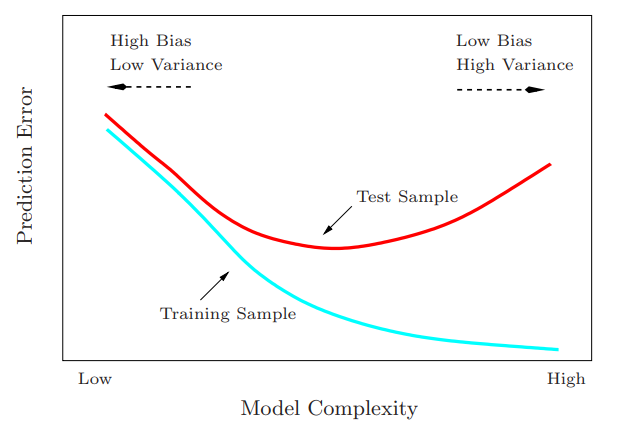
\includegraphics[width=1\linewidth]{figs/hastie.png}
    \caption{Test and training error as a function of model complexity. Taken from Hastie et al. \cite{hastie2009}}
    \label{fig:hastie_et_al}
\end{figure}


\subsection{Resampling Methods}

When we are working with one set of data, the train-test split will only give an estimate of the test error for that particular split. It is therefore dependent on which data ended up in the training split and gives no information of how the model would change if the training set looked different. Resampling methods work around this by using the same data to make multiple training sets and refitting the model for each of these. In this project we have used bootstrap and $k$-fold cross-validation.

\subsubsection{Bootstrap}\label{sec:bootstrap}

To study the bias and variance of the model as discussed in the section above, we need to know how the predictions vary over many different training sets. Instead of generating these directly, since we do not know how the data was distributed, we use the bootstrap resampling method.

The bootstrap is carried out as follows:
We randomly draw $n$ points from the training data in order to form a bootstrap sample. The same point can be drawn more than once. We train the model on the bootstrap sample and use it to predict the values at the test points. This is repeated n$\_$bootstraps times, in our case this was 100. And we get 100 different predictions for each test point. We can then derive the bias and variance from these predictions.

Since bootstrap resampling uses the same data set, on average, only 63.2$\%$ are unique observations whereas the remainders are duplicates. This leaves 36.8$\%$ as \textit{out-of-bag} observations and the training set will be smaller.

\subsubsection{$k$-fold Cross-validation}
In this project, two different methodologies were used for cross-validation, guided by different sources of information. For the initial implementation the data was split in k-folds with no training set, guided by the lecture book\cite{lecture_book}. The implementation for tuning hyperparameters, although remaining largely the same, implemented a test-train split, with k folds on the training data, guided by the scikit-learn user guide \cite{scikitlearn-crossvalidation}. Aside from the splitting of data, the initial implementation in \ref{sec:cv-first-implementation} is reused in the second implementation \ref{sec:cv-second-implementation}\\

\paragraph{Cross validation}\label{sec:cv-first-implementation}
$k$-fold cross validation reduces the dependence on a single train-test split by using the whole data set. The data is divided into $k$ subsets of roughly equal size called folds. Each of these folds takes turns being the test set while the remaining $k-1$ folds serve as the training set. Each observation is thus used for training $k-1$ times and for testing exactly once. This improves the ability to develop a model when the data is sparse, with the downside that it becomes more computationally expensive. As the dataset in this project is small, this is of no issue. 

The procedure is as follows. We first shuffle the data set at random, then split it into $k$ folds. For each fold, we set it aside and fit the model on the remaining folds and evaluate it on the fold that was set aside. We then record the score, also known as the cost function, and discard the model. The mean of the $k$ scores give the cross-validation MSE. The standard deviation of the $k$ scores shows how much the error varies between the folds \cite{lecture_book}.

When working with using $k$-fold cross-validation it is important that any preprocessing of the data must be performed inside the cross-validation loop. If we scale the data set before the loop, each training fold can see the mean and variance of its own test fold (i.e. data leak), causing the estimate of the error to be too optimistic.\\

\paragraph{Cross validation with hyperparameters}\label{sec:cv-second-implementation}

In the case where one wants to do a train-test split with cross-validation on the training split as in \cref{fig:scikitlearn-cross-validation}, the main procedure follows as in \ref{sec:cv-first-implementation}, but using the training data only for the cross-validation, giving the averaged MSE per cross-validation on the training set.

\begin{figure}
    \centering
    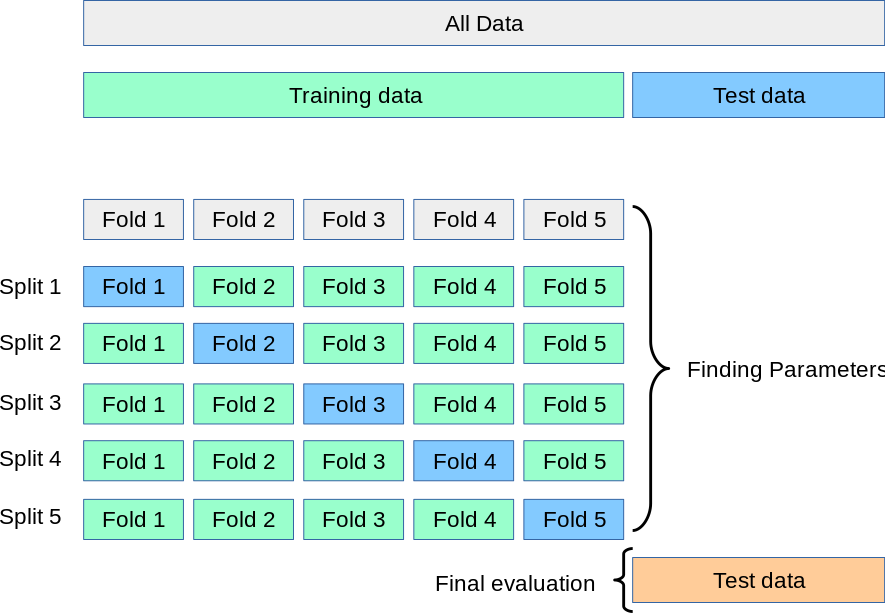
\includegraphics[width=1\linewidth]{figs/grid_search_cross_validation_scikitlearn.png}
    \caption{Visualisation of division of data using k-fold cross-validation\cite{scikitlearn-crossvalidation}}
    \label{fig:scikitlearn-cross-validation}
\end{figure}

As there are many different estimators in the machine learning world, such as OLS, Ridge and Lasso, one needs a way to compare them. They have different mathematical descriptions, with Ridge and Lasso having no direct point of comparison. Out of a selection of models, one can tune each parameter, so that the best model yields the best score out of possible parameters.

The search of such parameters is called tuning the hyperparameters, which in our case for Ridge, Lasso and OSL would be the degree, and for Ridge and Lasso the penalty $\lambda$. We apply the same cross-validation loop, but now over a grid of these hyperparameters. For each combination, the hyperparameters yielding the minimised cost function are stored and used to train a model on the whole train-split. We use this same model to calculate the test MSE using the test-split.

To validate, we compare the train and test MSEs. A test MSE that is close to the train MSE indicates that the model generalizes well with little overfitting to the training data \cite{scikitlearn-crossvalidation}. While the best model, this does not mean the cheapest. It is typical to then chose the best cheapest model, meaning for example fewer degrees, as long as the score of the model is within one standard error above the error of the best model \cite{hastie2009}.

MSE decomposition using the training set was also attempted as per the bootstrap method of Bias-Variance decomposition. Additionally, a resampling strategy using k-folds was also developed, where the splitting is as described in \cref{sec:cv-first-implementation}. Final fits were done on the whole dataset. 



\subsection{Optimizers}

We have now looked at different ways of finding the optimal parameters for our model, but how can minimize the cost of these parameters? To do this we will use different types of \textit{optimizers}, and study how well different optimizer methods perform in relation to each other. What an optimizer generally does is find the optimal parameter that minimises the cost function $C(\bm{\theta})$, but there are different ways to find a minimum. 

\subsubsection{Gradient descent code, with analytical gradients and automatic differentiation} % maria 

    Gradient descent is an optimization method used to optimize the model which describes our data. For any model we have, to describe a data set, there will be a cost function, $C(\mathbf{X}, g(\mathbf{\theta}))$, that tells us how far off from the truth our model is. Our goal is to minimize the cost function, so that our model is as close to the data set as possible. \\
    Gradient descent works by finding the gradient of a given point of the cost function, and then moving a \textit{small} increment in the negative direction of the gradient, so down toward the minimum. After we've moved a small step down, we calculate the gradient again and repeat the process. This process repeats until the slope of the gradient gets small enough for us to assume that we're on, or close to the minimum. We can write the method of gradient descent as 
    \begin{align}\label{eq: gradient descent}
        \bm{\theta}_{k + 1} = \bm{\theta}_k - \gamma\bm{ \nabla}_{\theta} C(\bm{\theta}_k),
    \end{align}
    where $\bm{\theta}$ is the optimal parameter, $k$ is the iteration number and $\gamma$ decides the length of the step we take between each time we calculate the gradient. In machine learning, we call this the \textit{learning rate}. The learning rate needs to be small enough, so that we don't overshoot the minimum by taking too large steps. But we also need to make sure it's not so small that our program efficiency is effected. In figure \ref{fig: GD illustration} an illustration of how the learning rate as a step size, decides where the program stops when approaching the minimum. 
    \begin{figure}[h!]
        \centering
        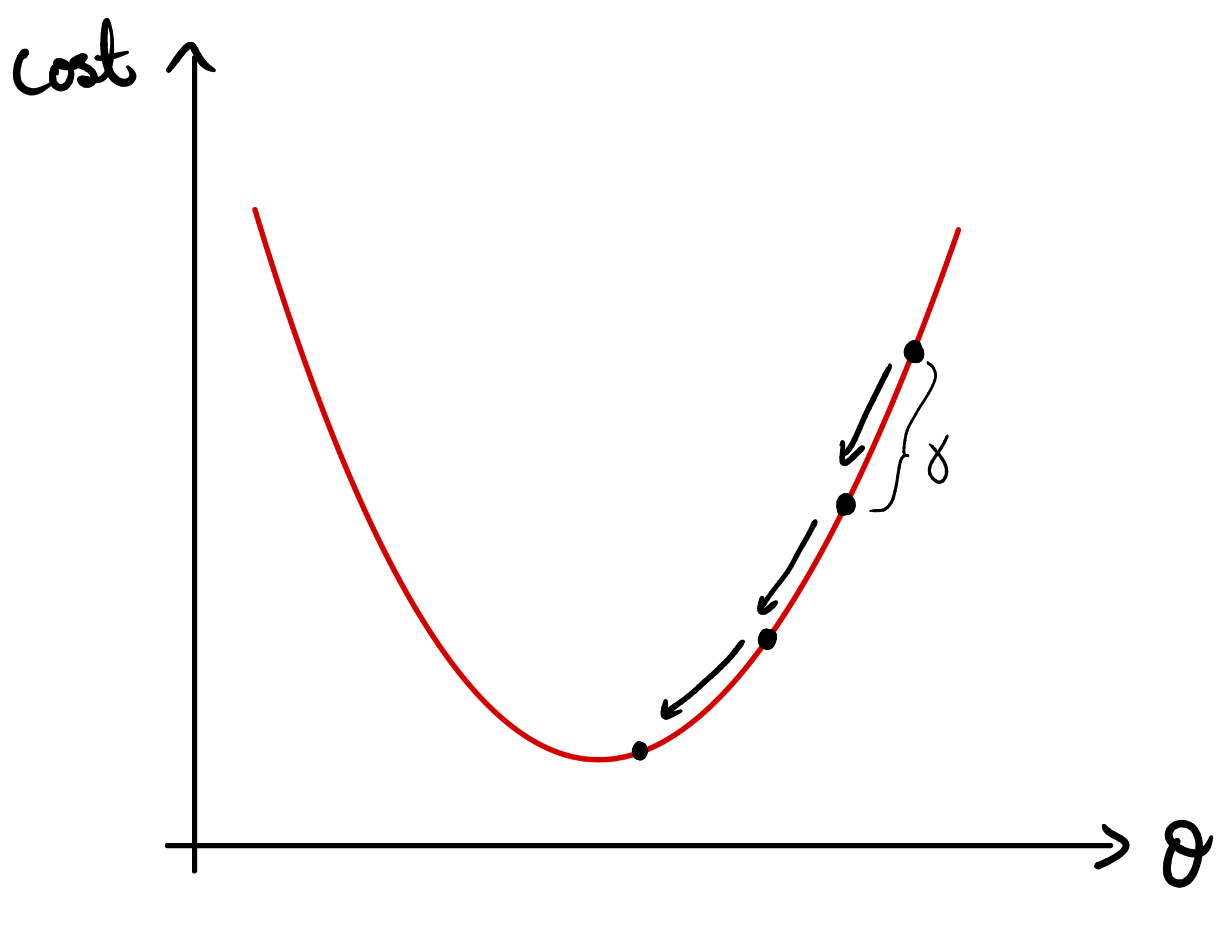
\includegraphics[width=0.9\linewidth]{figs/GD_illustration.jpg}
        \caption{Illustration of how gradient descent find the minimum with the learning rate $\gamma$ as the step size. }
        \label{fig: GD illustration}
    \end{figure}\\
    To find the limit of how large the learning rate can be $\gamma_{\text{max}}$ we use the equation 
    \begin{align}
        \gamma_{\text{max}} = \frac{2}{\lambda_{\text{max}} (\bm{H})},
    \end{align}
    where $\lambda_{\text{max}}(\bm{H})$ is the is the largest eigenvalue of the Hessian, given as
    \begin{align}
        \bm{H} = \frac{2}{n} \bm{X}^T\bm{X} + 2\lambda \bm{I},
    \end{align}
    where the factor with the penalty $\lambda$ is used for Ridge, and for OLS this factor disappears, as there is no penalty. \\
    The gradient of the cost function for linear regression (OLS) can be written as
    \begin{align}\label{eq: gradient of OLS}
        \bm{\nabla}_{\theta} C(\bm{\theta}_k) = \frac{2}{n} \bm{X}^T (\bm{X}\bm{\theta}_k - \bm{y}),
    \end{align}
    where $n$ is the number of data points, $\bm{X}$ is the design matrix of our model and $\bm{y}$ represents our target values. \\
    For Ridge regression we have an additional penalty term for the gradient, and we  will therefore express this as
    \begin{align}\label{eq: gradient for ridge}
        \bm{\nabla}_{\theta} C(\bm{\theta}_k) = \frac{2}{n} \bm{X}^T (\bm{X}\bm{\theta} - \bm{y}) + 2 \bm{\lambda}\bm{\theta},
    \end{align}
    where $\bm{\lambda}$ represents the penalization. \\
    For these gradient descent methods, we need to calculate the gradient of the cost function for every step we take. Doing this for large models is error-prone, and impractical. What we can do instead is use \textit{Automatic Differentiation} (AD), which essentially chains together the derivative of each step as it goes, instead of making a formula for the whole thing. This method utilizes the elementary operations, such as addition and multiplication, which the computer already knows. 

    

\subsubsection{Including momentum and more advanced ways to update the learning rate} % hannah
%

Using gradient decent has one major caveat. As the slope of the gradient decreases to a minimum, this might be the local minimum and not the global one. Additionally, as the learning rate of the method remains the same, a step that would be too big when the gradient is steep is hopelessly small along a flat one \cite{addition_w38}. 

To circumvent gradient decent error-prone and computationally expensive ways, dynamic versions have been implemented. The following methods have a dynamic step sizes, where previous steps \textit{remember} what came before them. By remember we mean their mathematical definitions make it so they retain the previous gradient $\nabla C(\bm{\theta})$ to some extent. Some also correct accordingly to its size and direction of  $\nabla C(\bm{\theta})$.

For the following methods, let the gradient of the cost function be \(g_t = \nabla C(\theta_{t-1})\), with \(v_0 = r_0 = m_0 = 0\). For vector parameters, squares, square roots, and division are elementwise.

\paragraph{Momentum}
\begin{equation}
\begin{aligned}
v_{t+1} &= \beta v_{t} + \gamma g_t, \\
\bm{\theta}_{t + 1} &= \bm{\theta}_t - v_{t+1},
\end{aligned}
\label{eq:momentum}
\end{equation}
where $v_t$ can be seen as the velocity or accumulator, $\gamma$ is the base learning rate and $\beta$ is the momentum coefficient with a typical value of 0.9, with $t$ denoting as step of the method. In the following, gradient method parameters have the same meaning unless stated otherwise. 

In the momentum gradient descent \eqref{eq:momentum} \cite{addition_w38}, we extend the definition of the step length. In plain gradient descent we have the step length solely determined by $\lambda g_t$, while in momentum this is determined by $v_{t+1}$. The parameter $v_t$ can be seen as the velocity, giving the method name momentum. As the gradient $g_t$ grows or decreases, the step size follows $v_{t+1}$, giving the name momentum. When the gradient is steep, the steps are large and vice versa.

Some downsides of momentum are that it can overshoot and therefore oscillate before $\bm{\theta}_t$ reduces to the set tolerance, giving higher number of oscillations.  As $v_{t+1}$ depends on $g_t$ and no previous step is forgotten, a major change in the gradient can take many iterations. The more complex the plane becomes, the more important these issues this are.

The highest learning rate for momentum is given by $\gamma_\text{max} = 2(1+\beta)/\lambda_\text{max}$ where $\lambda_\text{max}$ is the largest eigenvalue of the hessian.

\paragraph{AdaGrad}
\begin{equation}
\begin{aligned}
r_{t+1,j} &= r_{t,j} + g_{t,j} \odot g_{t,j}, \\
\bm{\theta}_{t+1,j} &= \bm{\theta}_{t,j}
 -  \frac{\gamma}{\sqrt{r_{t,j}}+\varepsilon}g_{t,j}
\end{aligned}
\label{eq:adagrad}
\end{equation}
where $t,j$ denotes that each feature has its own parameters. $r_{t+1,j}$ is the accumulator. 

AdaGrad \eqref{eq:adagrad} builds on a similar adaptive step size as momentum, but tunes each parameter $\bm{\theta}_{t,j}$ separately. This means that through $g_t \odot g_T$, frequent features have smaller step sized while sparse features have a bigger impact. The intent of AdaGrad exactly this, to train models that have sparse features.

A consequence of $g_t \odot g_T$ is that $r_{t}$ never decreases. As a result the step size determined by $\frac{\gamma}{\sqrt{\varepsilon + r_t,j}}$ always decreases. Eventually it may come to a halt even if the best $\bm{\theta}_{t,j}$ has not been reached. In convex problems such as the ones which we address in this project this is tolerable, but in cases like deep learning where the landscapes aren't convex, AdaGrad simply stops \cite{addition_w38}.


\paragraph{RMSProp}
\begin{equation}
\begin{aligned}
v_{t} &= \rho v_{t-1} + (1-\rho)g_t^2, \\
\bm{\theta}_{t+1} &= \bm{\theta}_{t}
 - \frac{\gamma }{\sqrt{v_{t}+\varepsilon}}g_t
\end{aligned}
\label{eq:rmsprop}
\end{equation}
with $\rho$ being the decay rate and $\varepsilon$ being the stabilizer.

RMSProp \eqref{eq:rmsprop} attempts to fix AdaGrad's eternal retention issue. With the term $(1-\rho)g_t$ the gradient becomes weighted and exponentially decreasing. With $\rho = 0.9$ this means that the current step $\bm{\theta}_t$ remembers the 10 previous steps. This fixes the issue that AdaGrad has with penalizing features forever if they had big gradients early in the training process, but retains the usefulness for sparse features. 

An issue with RMSProp lies in the start when $v_0=0$. This gives $v_{1}=(1-\rho)g_t^2$, heavily biasing the initial steps. This might make it overshoot early in the training, resulting in instability, especially when $\rho$ is close to 1. At the same time, for sparse features when $v_t$ is nearly 0 before a new occurrence, weighing sparse features more heavily due to these large steps. 


\paragraph{Adam}
\begin{equation}
\begin{aligned}
m_{t+1} &= \beta_1 m_{t-1} + (1-\beta_1)g_t, \\
r_{t+1} &= \beta_2 v_{t-1} + (1-\beta_2)(g_t)^2, \\\\
\hat{m}_{t} &= \frac{m_{t}}{1-\beta_1^t}  \qquad
\hat{r}_{t} = \frac{r_{t}}{1-\beta_2^t} \\
\label{eq:adam_parts}
\end{aligned}
\end{equation}
where $m_t$ is the momentum term and $r_t$ is the RMS term. $\beta_1$ is the momentum decay and $\beta_2$ is the decay applied to the RMS term, with typical values $\beta_1 = 0.9$ and $\beta_2 = 0.999$. 

Adam \eqref{eq:adam} can be seen as a combination of momentum and RMSProp. The momentum term $m_{t+1}$ accelerates the learning when the gradient is consistent along one direction, while the RMS term $v_{t+1}$ dampens as size of the gradient $g_t$ decreases. 


\begin{equation}
\begin{aligned}
\bm{\theta}_{t+1} &= \bm{\theta}_{t}
 - \gamma \frac{\hat{m}_{t}}{\sqrt{\hat{r}_{t}}+\varepsilon}
\end{aligned}
\label{eq:adam}
\end{equation}

To account for the RMSProp behaviour that leads to biasing for initial steps, the terms $\hat{m}_t$ and $\hat{v}_t$ include a bias correction. Adam yields a combined adaptive learning method including the best features from momentum and RMSProp while also correcting for their disadvantages with \eqref{eq:adam} \cite{addition_w38}.  

In this project these methods \cref{eq:momentum,eq:adagrad,eq:rmsprop,eq:adam} are implemented using the modules Optax and JAX. Note how the meaning of the learning rate $\lambda$ changes dependent on how they are implemented in each model. To showcase this, we will see how many iterations are needed to reach set tolerances. 




\subsubsection{Stochastic gradient descent } % maria
    There are different ways to optimize a model, based on what you wish to accomplish by optimizing. When we're looking at a model that has $n = 100$ data points, we don't really think about the cost of running the program, as it won't be large. But when we instead start working with large models, such as neural networks, the cost of running the program will be significant. \\
    Stochastic gradient descent (SGD) tackles the cost of a model, by making each step cheaper and accepts a noisy direction as the price. We will take account for both of these factors when making our SGD code, so that we don't end up with the cheapest model, but also the noisiest so that there's no accuracy in the model. \\
    SGD works by implementing a random subset of the data, called a \textit{mini batch}, and finding the gradient of this mini batch. We can decide the size of the mini batches $M$, for the $n$ data points, which will give $n/M$ number of mini batches. As in equation \ref{eq: gradient descent}, we have the same method for updating the optimal parameter for SGD, but now per mini batch. The update becomes
    \begin{align}\label{eq: SGD}
        \bm{\theta}_{t + 1} = \bm{\theta}_t - \frac{\gamma_t}{M} \nabla C(\bm{\theta}_t),
    \end{align}
    where $\nabla C(\bm{\theta}_t)$ is the gradient of the cost function used, in the same way as we did for the standard gradient descent method.\\
    If we have 10 mini batches for $n = 100$ data points, there will be 10 data points in each batch. When these mini batches have been passed over, this is called an \textit{epoch}. We can decide how many epochs we want to run, and for each epoch that is ran, the mini batches will be randomly shuffled. \\
    To study how sensitive SGD is to the learning rate schedule itself, rather than using a single $\gamma$, we also implement a decaying schedule given as
    \begin{align}\label{eq: decaying schedule}
        \gamma_t = \frac{t_0}{t + t_1},
    \end{align}
    where $t$ is the current step number, and $t_0$ and $t_1$ together are the free parameters that control the schedules behaviour. Rather than keeping the learning rate $\gamma$ fixed when training the data, the decaying schedule lets it shrink as training progresses. $\gamma_t$ is largest for the very first step, and decreases toward zero as the steps $t$ go on. This is useful because we want to take large steps at the very start, when we're far away from the minimum, but as we get closer we want to take smaller steps in order to get as close as possible. In figure \ref{fig: SGD decay schedule} an illustration of how the decaying schedule looks when searching for the minimum.
    \begin{figure}[h!]
        \centering
        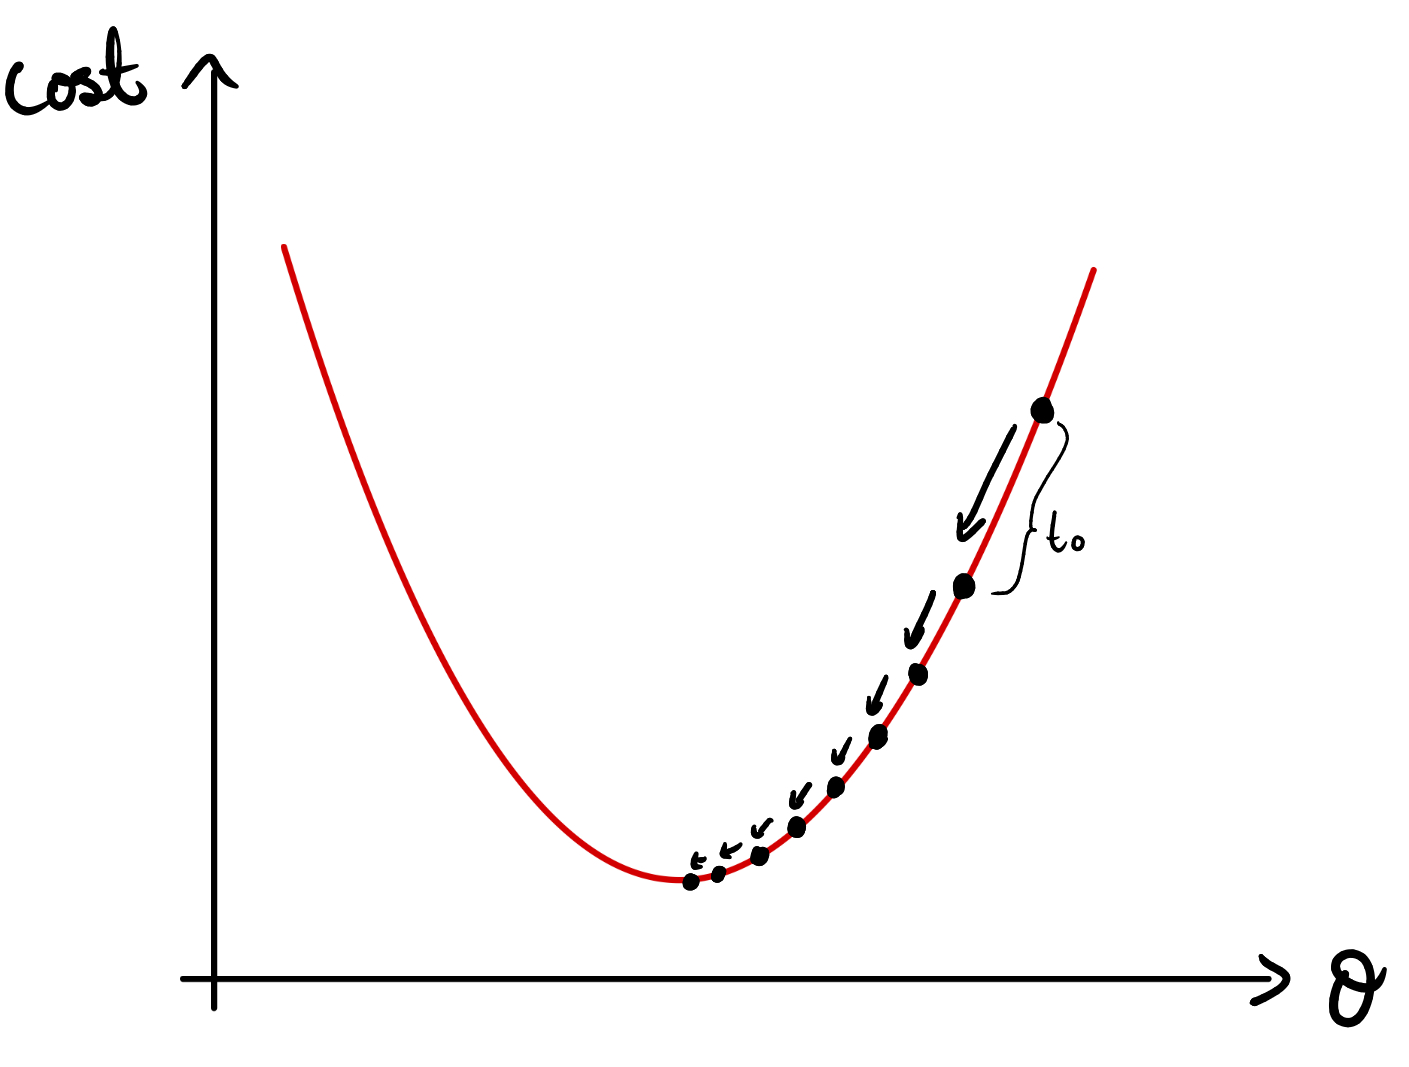
\includegraphics[width=0.9\linewidth]{figs/SGD_decay_schedule.jpg}
        \caption{Illustration of the decaying schedule used for stochastic gradient descent. }
        \label{fig: SGD decay schedule}
    \end{figure}\\
    The parameter $t_0$ decides the initial step size, and $t_1$ decides for how many steps the learning rate stays close to its initial value before decay becomes significant. When deciding $t_1$, the total number of steps that will run need to be taken account for. If $t_1$ is small compared to the number of steps, $\gamma_t$ will decay to a negligible value before the training is complete, and the schedule will underperform. 
    
\section{Results}\label{sec:Results}



\subsection{Ordinary Least Squares (OLS) for the Runge function}% nille


For OLS we see in Figure \ref{fig:part_a_OLS_polynomial} how the polynomial degrees affect the MSE and $R^2$ scores as well as the coefficient $\| \theta \|_2$. The noise floor is $\sigma^2$ and marked in a black dotted line at 0.01. The lowest test MSE is: 1.871 $\times 10^{-2}$ and the highest $R^2$ score is 0.8489, both at degree 8 which is marked with a grey dashed line.

\begin{figure}[h!]
    \centering
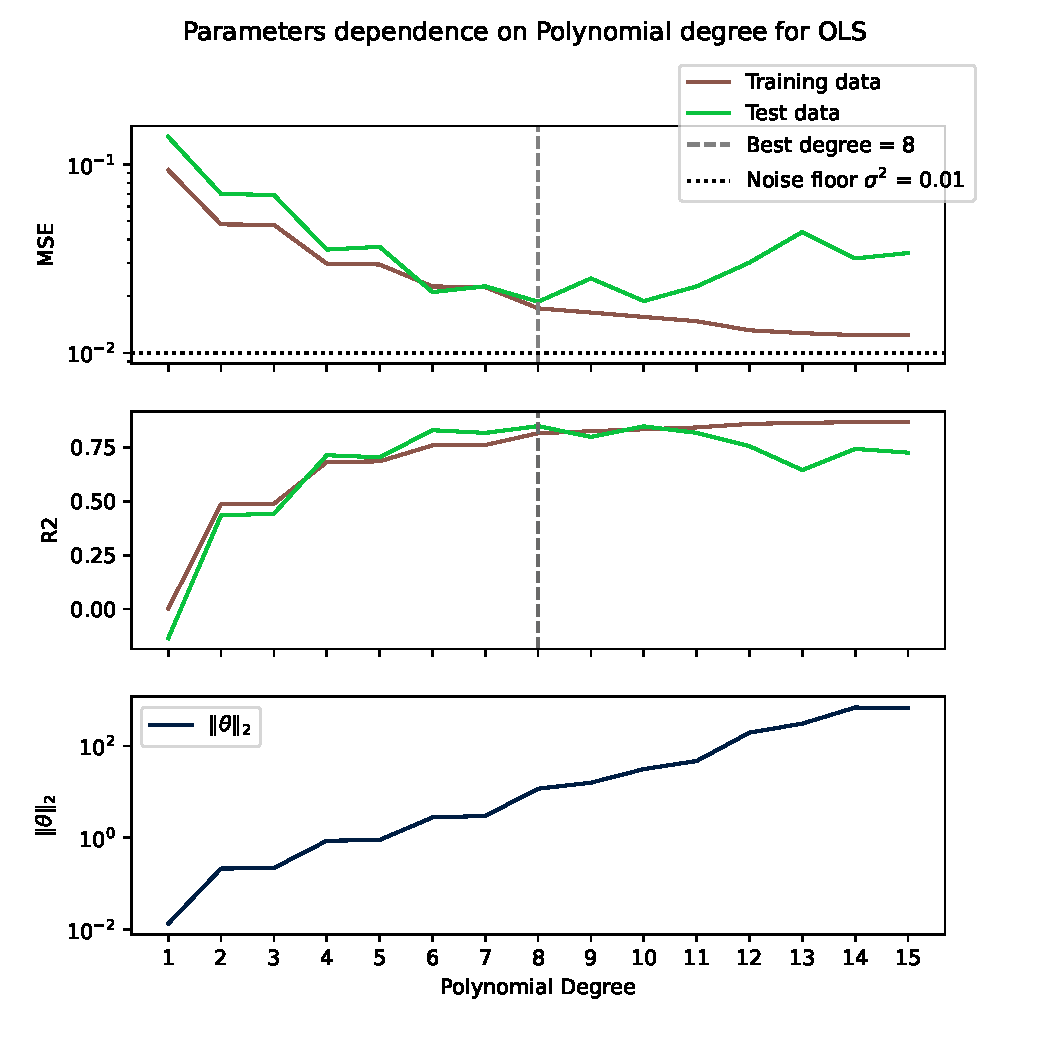
\includegraphics[width=\linewidth]{figs/Part_a_Paramets_over_polynomial.pdf}
    \caption{Test MSE is minimal and $R^2$ Score is maximal at degree 8. After this the test MSE increases while the training MSE decreases whereas the $R^2$ score does the opposite, indicating overfitting. The $\| \theta \|_2$ shows the overall magnitude of the coefficient vector as a single number per polynomial degree}
\label{fig:part_a_OLS_polynomial}
\end{figure}

We repeat the analysis at degree 8 for 15 values of $n$ in the interval [40,4000] and 10 noise levels $\sigma \in$ [0.01, 1], this can be showed in Figure \ref{fig:part_a_ols_heat_map}.  

The lowest test MSE is 3.309 $\times 10^{-3}$ is found for n = 4000 and $\sigma$= 0.01. While the highest test $R^2$ score is 0.9562 found for n = 322 and $\sigma$= 0.01. These are marked in the heatmap which shows the test MSE and R2 with 2 significant digits.



\begin{figure}[h!]
    \centering
    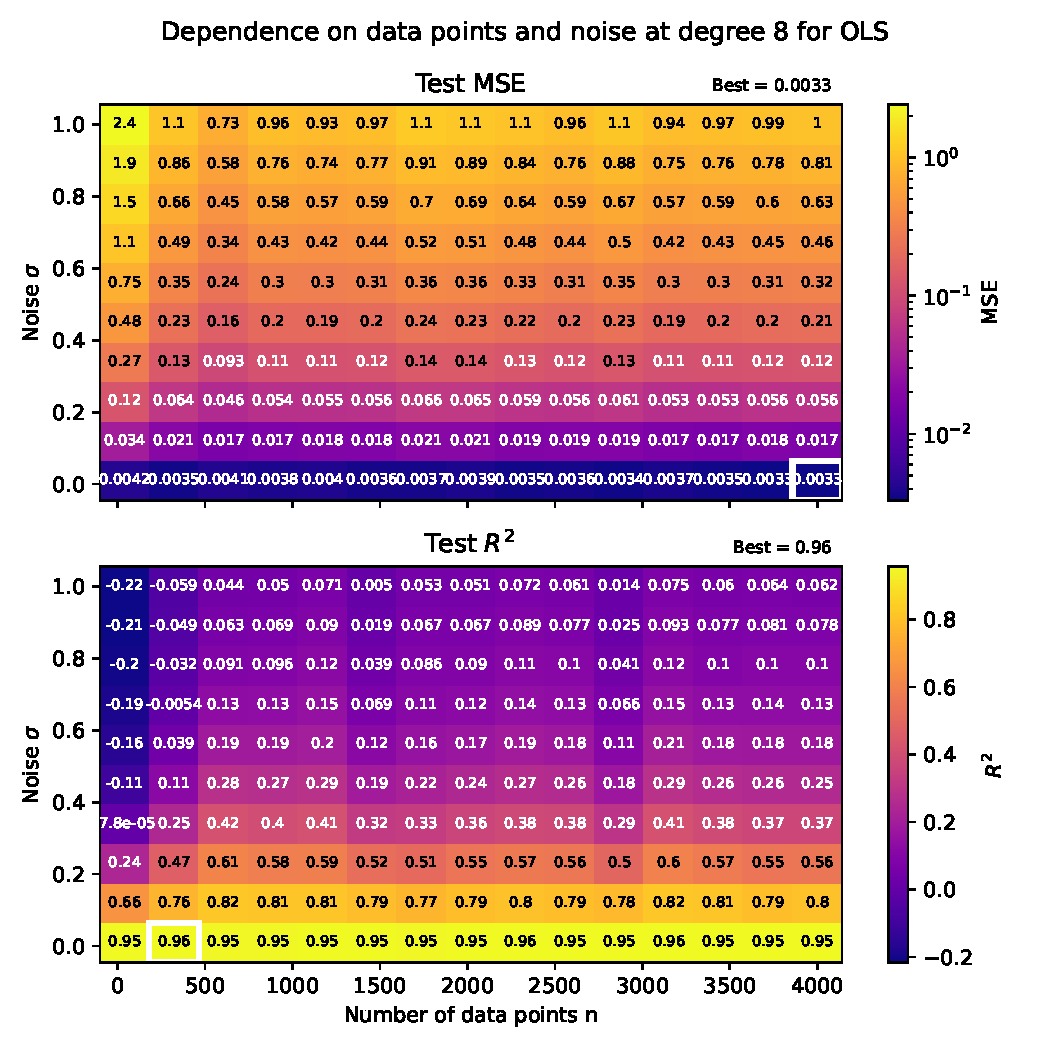
\includegraphics[width=\linewidth]{figs/Part_a_heatmaps_MSE_R2.pdf}
    \caption{The lowest test MSE at 3.309 $\times 10^{-3}$ at n = 4000 and $\sigma$= 0.01. The best test $R^2$ score at 0.9562 at n = 322 and $\sigma$= 0.01}
\label{fig:part_a_ols_heat_map}
\end{figure}

We can see how the OLS coefficients $\theta_j$ behave as a function of the degree of the polynomial in Figure \ref{fig:ols_theta_coeffs} 

\begin{figure}[h!]
    \centering
    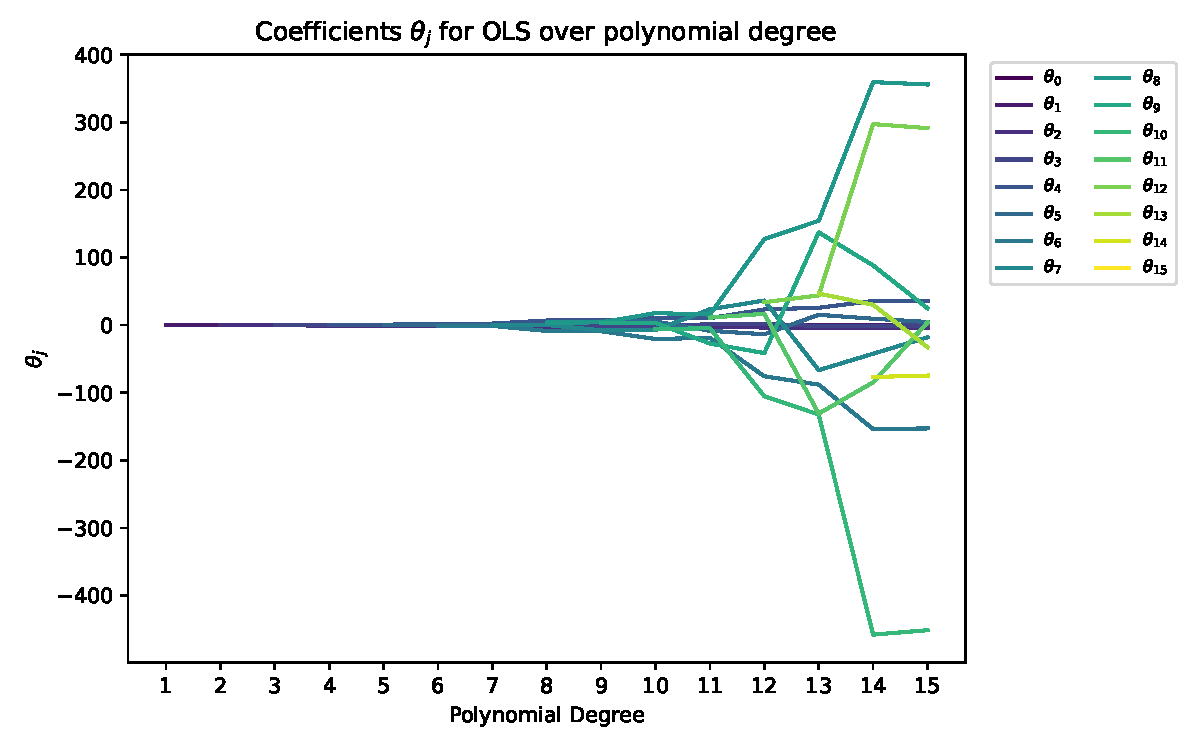
\includegraphics[width=\linewidth]{figs/Part_a_theta_coeff.pdf}
    \caption{Coefficients stay small at a low polynomial degree and blow up at higher degrees, which is consitent with the overfitting seen in Figure \ref{fig:part_a_OLS_polynomial}.}
    \label{fig:ols_theta_coeffs}
\end{figure}


\subsection{Adding Ridge regression for the Runge function}% nille

An analysis of how the MSE, $R^2$ scores and $\| \theta \|_2$ change over different $\lambda$ values for a polynomial of degree 15 can be viewed in Figure \ref{fig:part_b_ridge_params_lambda}. The best $\lambda$ was extracted the same way as the best polynomial degree was for OLS and gave the best $\lambda$ at 0.040. This gives the lowest test MSE at 2.562 $\times 10^{-2}$, and the highest $R^2$score at 0.7931 with effective degrees of freedom at 7.78.

\begin{figure}[h!]
    \centering
    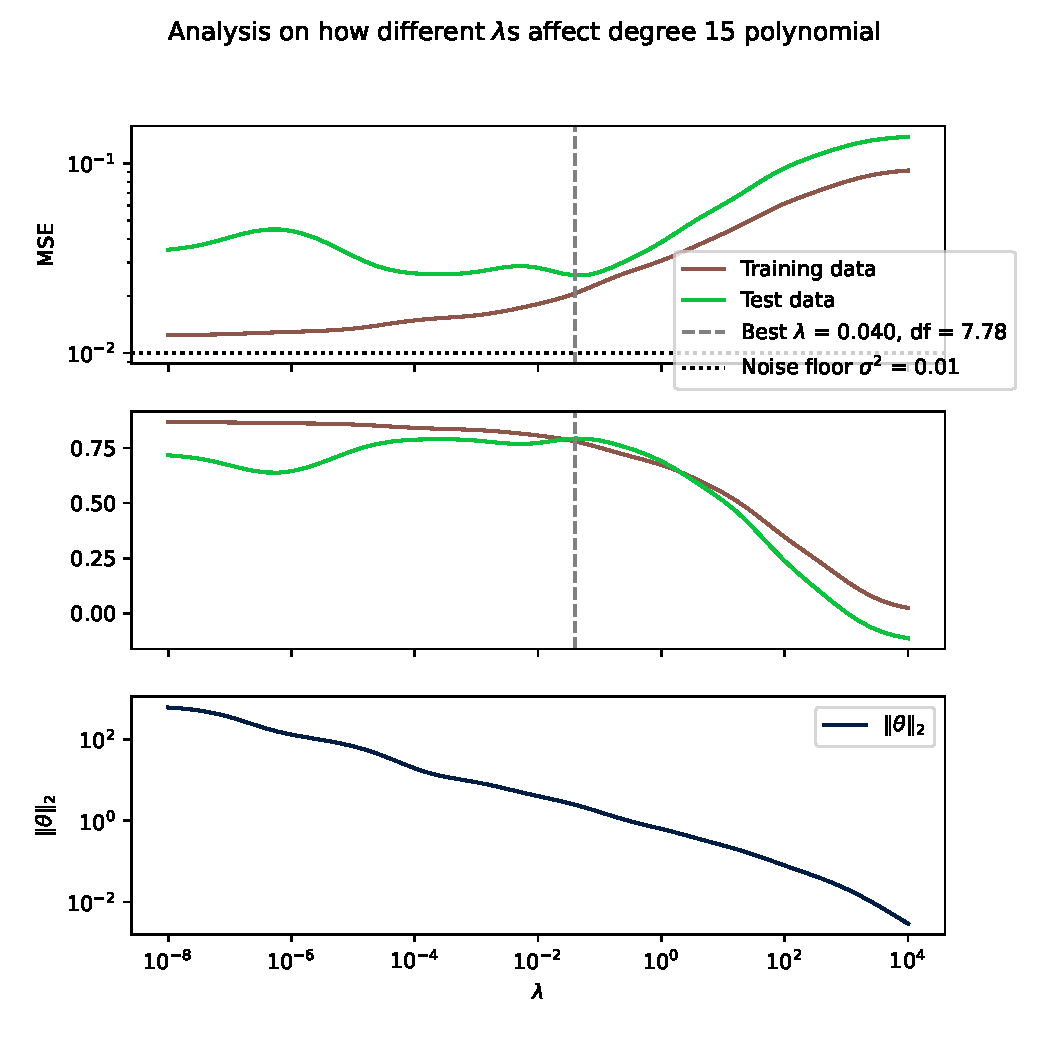
\includegraphics[width=\linewidth]{figs/Part_b_Params_vs_lambda.pdf}
    \caption{The best $\lambda$ = 0.040 with a degree of freedom at 7.78. The $\| \theta \|_2$ shows the overall magnitude of the coefficient vector as a single number per value of $\lambda$}
    \label{fig:part_b_ridge_params_lambda}
\end{figure}

The coefficients $\theta_j$ were analysed as a function of $\lambda$ in order to get a scope of how the penalty parameter $\lambda$ affects the magnitude of the coefficients $\theta_j$. This can be viewed in Figure \ref{fig:part_b_thetavs_lambda}.


\begin{figure}[h!]
    \centering
    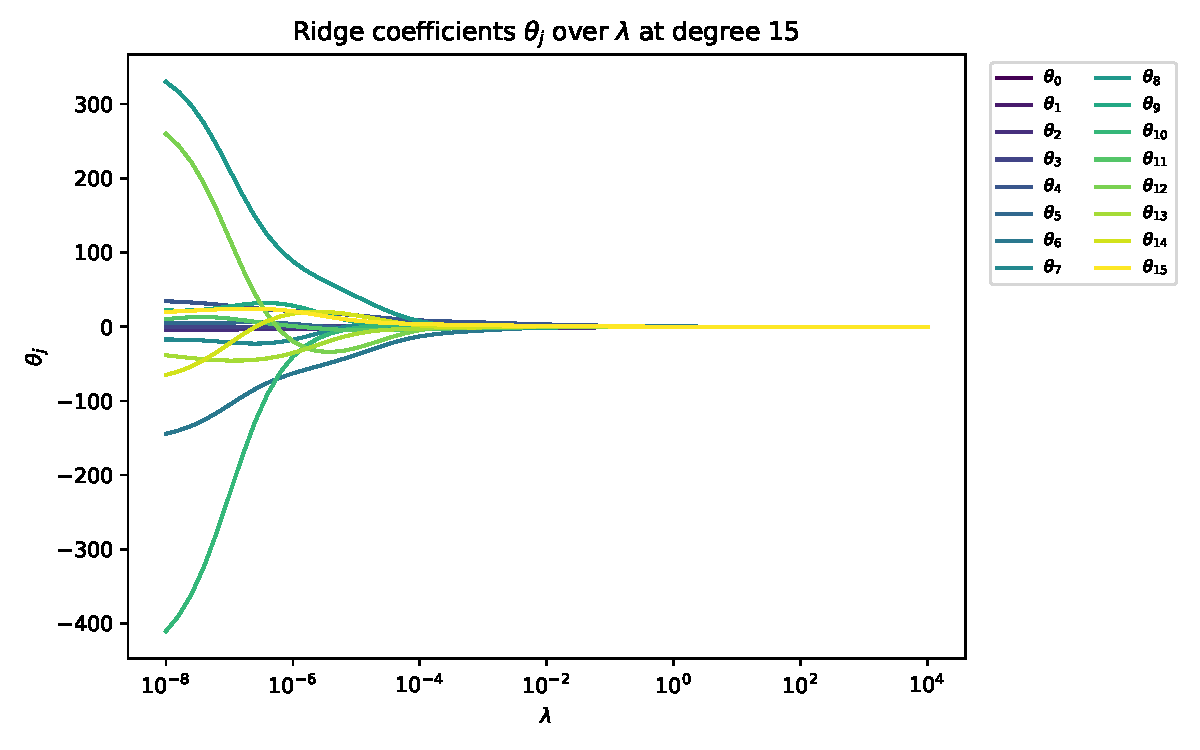
\includegraphics[width=\linewidth]{figs/Part_b_theta_vs_lambda.pdf}
    \caption{For smaller $\lambda$'s the solution looks like OLS (see Figure \ref{fig:ols_theta_coeffs}) with large values for the coefficients $\theta_j$. As $\lambda$ increases, these coefficients shrink.}
\label{fig:part_b_thetavs_lambda}
\end{figure}



Despite $\lambda$=0.040 is the best for a polynomial of degree 15, we continue to use it forward since we want to analyze how the MSE, $R^2$ and $\| \theta \|_2$ behave over polynomial degree. This can be viewed in Figure \ref{fig:part_b_param_vs_degree}. The lowest MSE is 2.323 $\times 10^{-2}$ and the highest $R^2$ score is 0.8125 at the best polynomial degree 12. 


\begin{figure}[h!]
    \centering
    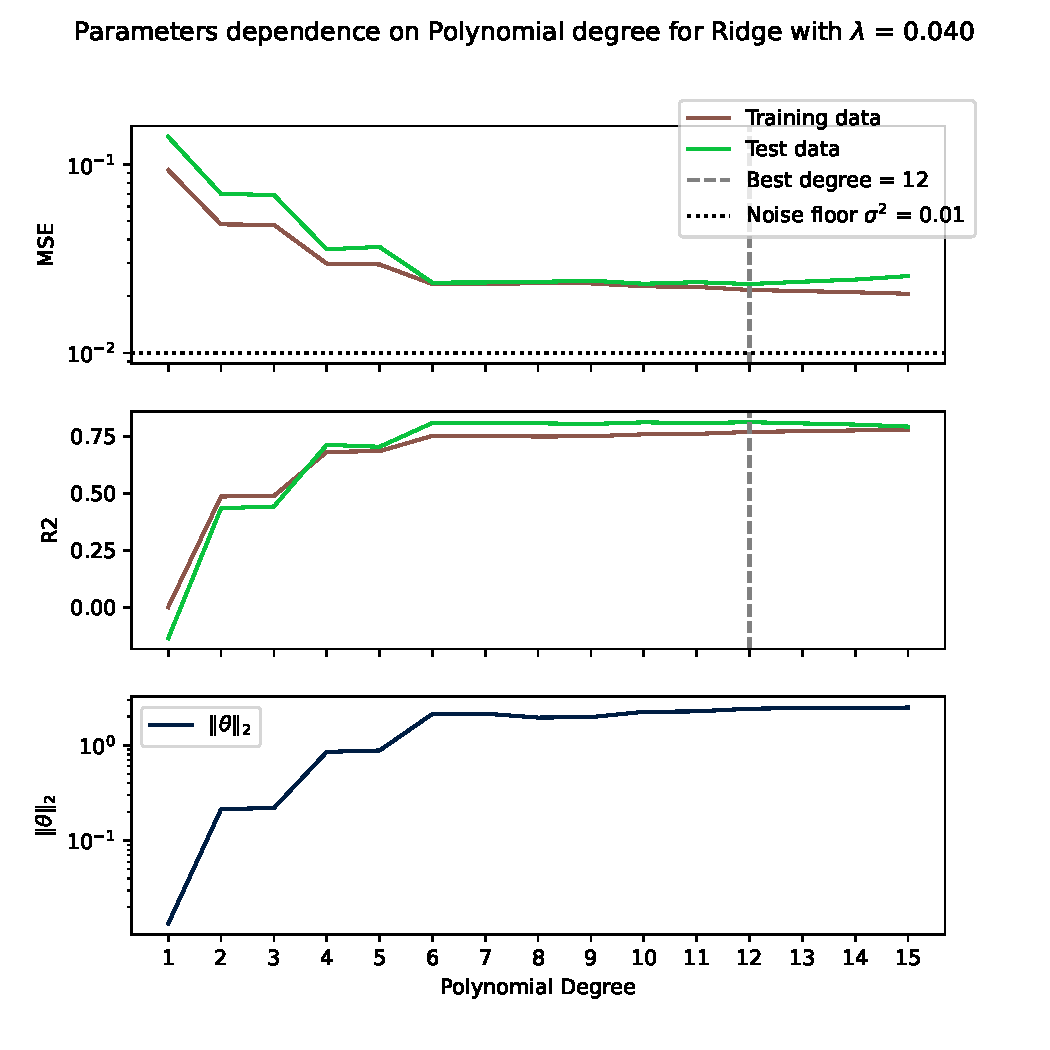
\includegraphics[width=\linewidth]{figs/Part_b_Parms_vs_degree.pdf}
    \caption{Test MSE is minimal and $R^2$ score is maximal at degree 12. The penalty parameter keeps the test MSE from blowing up and the training MSE from decreasing towards the noise floor in the same degree range as OLS seen in Figure \ref{fig:part_a_OLS_polynomial}}
    \label{fig:part_b_param_vs_degree}
\end{figure}

As done for OLS, we visualized the dependence on number of data points and noise over the same span. This was done by using the best polynomial degree and the best $\lambda$ and the results are shown in Figure \ref{fig:part_b_heatmap}. The lowest test MSE is 2.936 $\times 10^{-3}$ for n = 4000 and $\sigma$ = 0.01 and the highest $R^2$ score is 0.9599 for n = 4000 and $\sigma$ = 0.01.

\begin{figure}[h!]
    \centering
    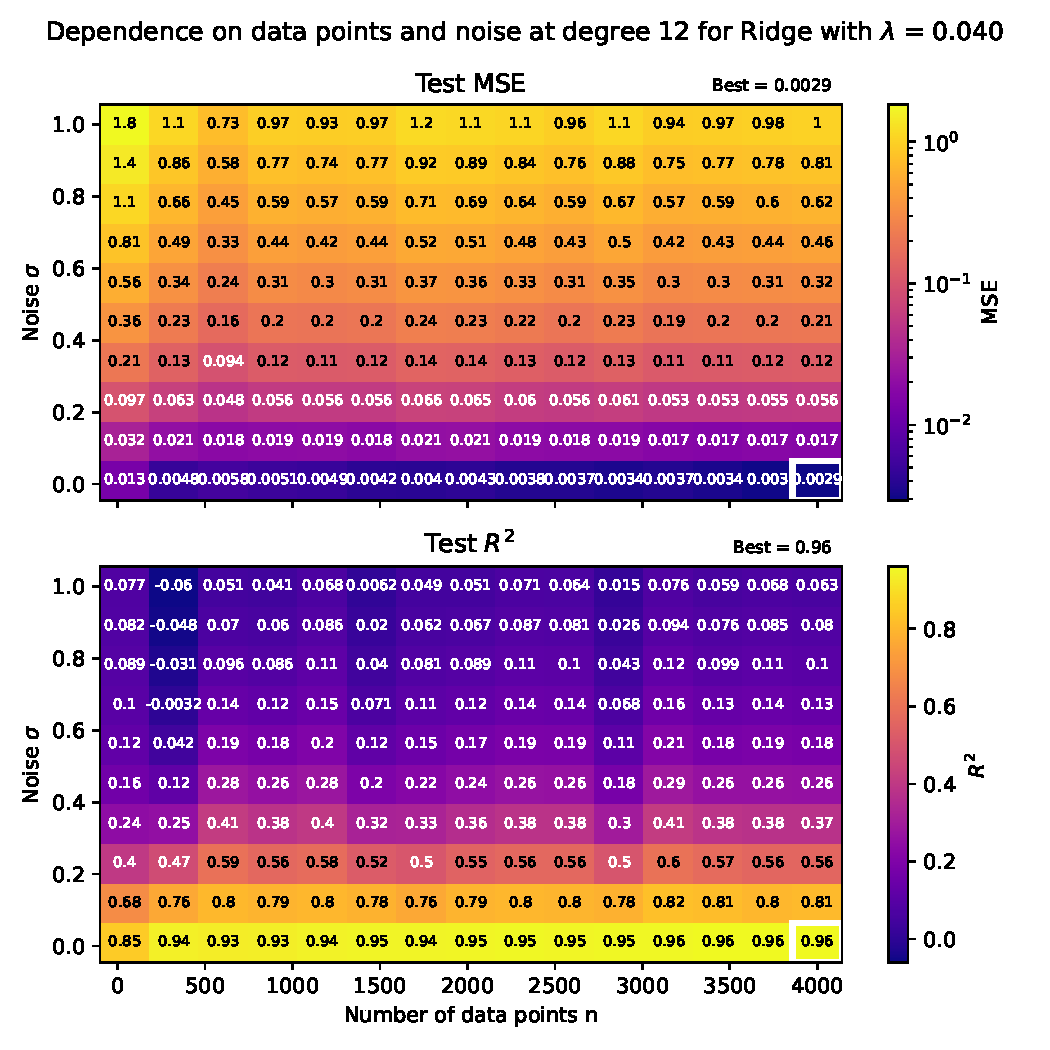
\includegraphics[width=\linewidth]{figs/Part_b_heatmaps_MSE_R2.pdf}
    \caption{Lowest test MSE at 2.936 $\times 10^{-3}$ with n = 4000 and $\sigma$ = 0.01. The highest $R^2$score at 0.9599 at n=4000 and $\sigma$=0.01}
    \label{fig:part_b_heatmap}
\end{figure}

The coefficients $\theta_j$ as a function of polynomial degree are shown in Figure  \ref{fig:ridge_theta_coeff} in the appendix \ref{app:more_figs}.

\subsection{The bias-variance trade-off and the bootstrap}% nille

We recreated Figure 2.11 from Hastie, et al \cite{hastie2009} in Figure \ref{fig:part_c_2.11} by extending the degree up to 20 to see the test error grow. 

\begin{figure}[h!]
    \centering
    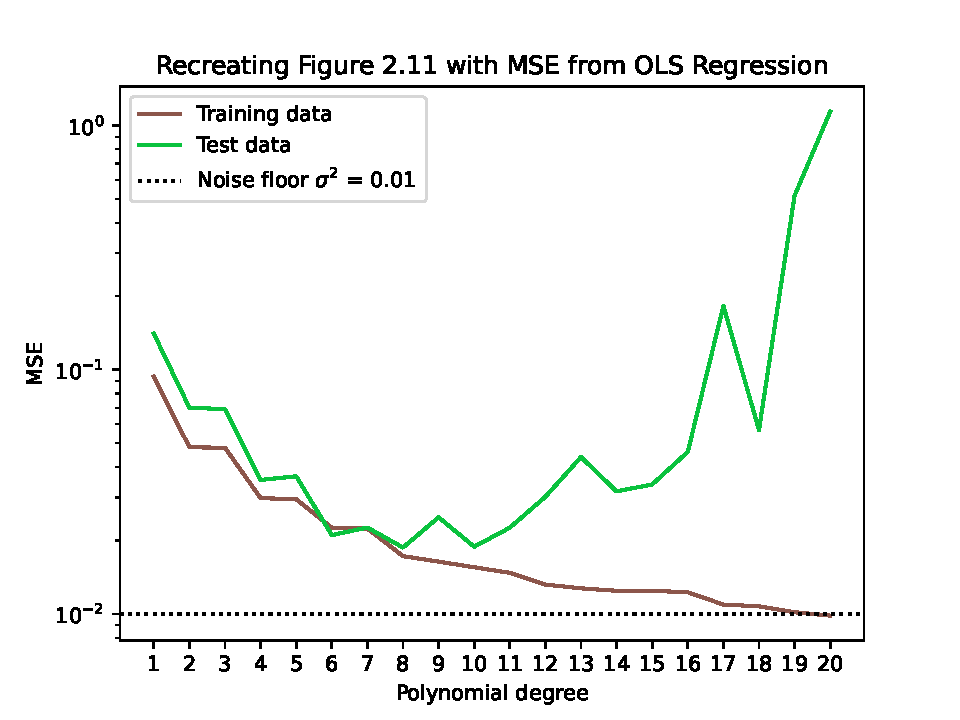
\includegraphics[width=\linewidth]{figs/Part_c_recreate_2.11.pdf}
    \caption{Recreation of Fig 2.11, Hastie et al. \cite{hastie2009} to visualize how model complexity affects test and training error}
    \label{fig:part_c_2.11}
\end{figure}

The bias-variance tradeoff using the bootstrap resampling technique using simpler ordinary least squares for polynomial degrees 1-15 with the number of bootstraps set to 100. This is shown in Figure \ref{fig:part_c_bootstrap}. It marks the best polynomial degree at degree 8 for bootstrap which has the lowest MSE at 3.328 $\times 10^{-2}$. It also plots the test MSE for OLS regression for comparison. The lowest test MSE for the OLS is 1.871 $\times 10^{-2}$ which is the same as values derived from Figure \ref{fig:part_a_OLS_polynomial}. 

\begin{figure}[h!]
    \centering
    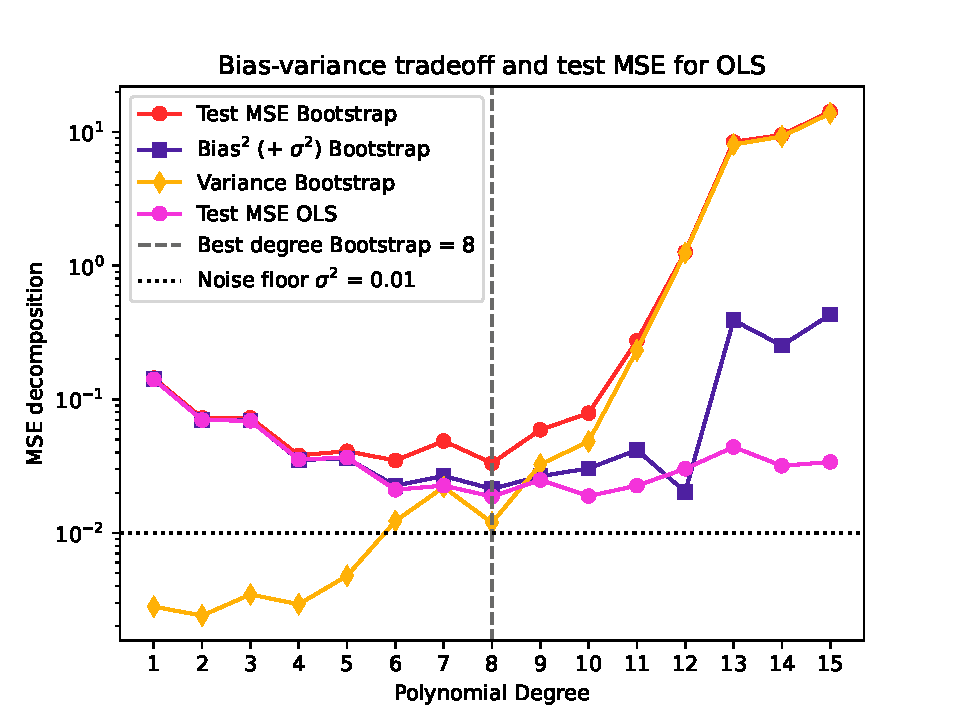
\includegraphics[width=\linewidth]{figs/Part_c_bootstrap.pdf}
    \caption{The best polynomial degree for simpler OLS bootstrap resampling is degree 8 where the test MSE is minimal. After this the variance shoots up and the bias has a spike after degree 12.}
    \label{fig:part_c_bootstrap}
\end{figure}

Three different plots with n=40, n=100 and n=400 were made in order to analyze how the bias-variance tradeoff changes depending on the number of data points used but still using the same number of bootstraps at 100. This can be viewed in Figure \ref{fig:part_c_bootstrap_ns}.

\begin{figure}[h!]
    \centering
    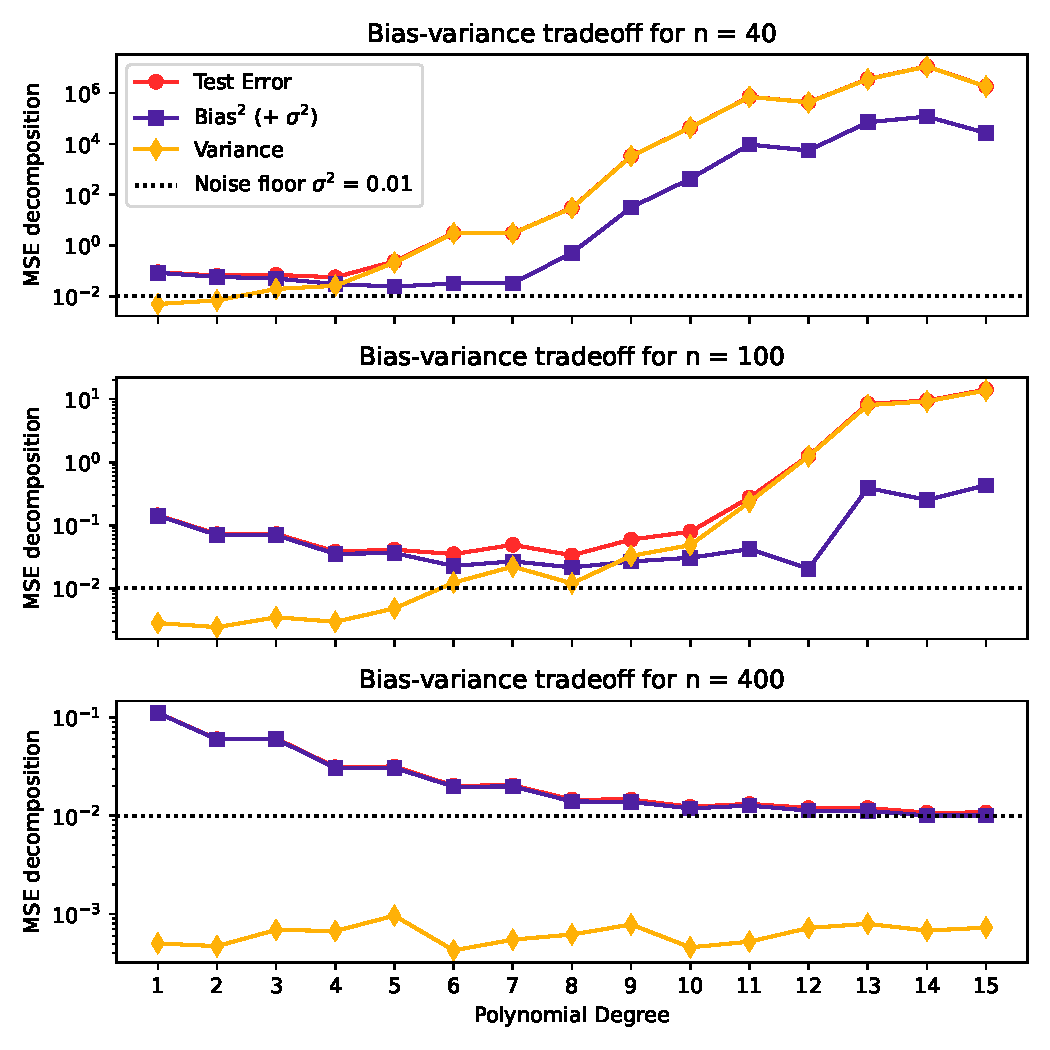
\includegraphics[width=\linewidth]{figs/Part_c_bootstrap_diff_ns.pdf}
    \caption{Using more data points (n) decreases the variance drastically so the test error will follow the bias despite the complexity of the model}
\label{fig:part_c_bootstrap_ns}
\end{figure}


\subsection{Cross-validation as a resampling technique}% nille

In Figure \ref{fig:part_d_comparsion}, the MSE using the $k$-fold cross-validation resampling technique with k = 5 and k = 10 is compared against the MSE collected from the bootstrap resampling method. Both use simpler OLS as the linear regression method. The cross validated MSE are plotted with error bars that show the $\pm 1$ standard deviation of the MSE across the $k$-folds. The cross-validated-points for the MSE are shifted slightly from their correct degree to better visualize how k = 5 and k = 10 differ over the folds. 


\begin{figure}[h!]
    \centering
    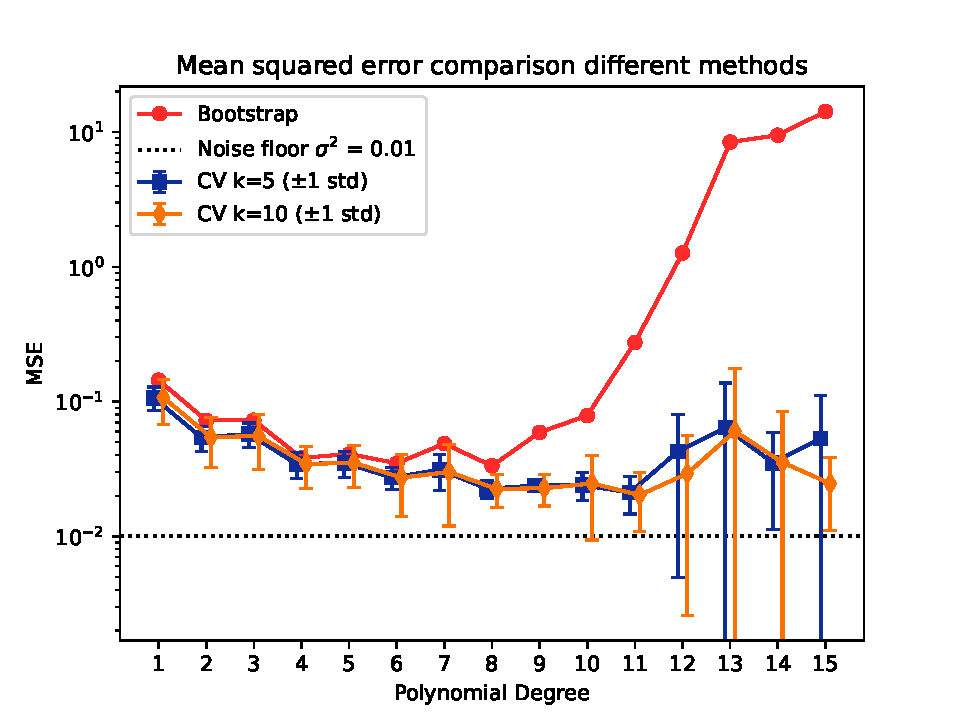
\includegraphics[width=\linewidth]{figs/Part_d_MSE_comparison.pdf}
    \caption{The three resampling methods give similar MSE scores from degree 1-8. Afterwards the bootstrap spikes and the curves for the cross-validated estimates stay almost flat until degree 11. From degree 12 the cross-validated estimates spike.  Both cross-validated curves decrease again after degree 13, but cross-validated with k = 5 has another spike after degree 14, whereas the cross-validated with k = 10 continues decreasing}
    \label{fig:part_d_comparsion}
\end{figure}

The subsequent best polynomial degrees and the lowest MSE derived from the data which makes up Figure \ref{fig:part_d_comparsion} are displayed in Table \ref{tab:part_d_best_degree_ols}.

\begin{table}[htbp]
    \centering
    \caption{Best polynomial degree and MSE for resampling techniques: bootstrap and $k$-fold cross-validation using linear regression method OLS.
    For cross-validation the uncertainty is $\pm 1$ std of the MSE across the $k$ folds.}
    \label{tab:part_d_best_degree_ols}
    \begin{tabular}{lcc}
        \toprule
        Method & Best degree & MSE ($\times 10^{-2}$) \\
        \midrule
        Bootstrap      & 8  & $3.328$ \\
        CV, $k = 5$    & 11 & $2.111 \pm 0.65$ \\
        CV, $k = 10$   & 11 & $2.024 \pm 0.93$ \\
        \bottomrule
    \end{tabular}
\end{table}

We then replace OLS by Ridge regression and study the dependence on the polynomial degree and the penalty parameter $\lambda$. We do this for $k$-fold cross-validation with k = 5 and k = 10 for 100 points of  $\lambda \in$ [$10^{-8}, 10^4$]. The best $\lambda$ values and the lowest cross-validated MSE for each polynomial degree are shown in Table \ref{tab:part_d_ridge_cv_lambda}.

\begin{table*}[htbp]
    \centering
    \caption{The best cross-validated MSE is (2.068 $\pm 0.54) $ $\times 10^{-2}$ for k = 5 folds and (1.918 $ \pm 0.78)\times 10^{-2}$ for k = 10 folds over the interval [$10^{-8}, 10^4$] for $\lambda$}
    \label{tab:part_d_ridge_cv_lambda}
    \begin{tabular}{c cc cc}
        \toprule
        & \multicolumn{2}{c}{\textbf{Best $\lambda$}} & \multicolumn{2}{c}{\textbf{CV-MSE} ($\times 10^{-2}$)} \\
        \cmidrule(lr){2-3} \cmidrule(lr){4-5}
        \textbf{Degree} & $k = 5$ & $k = 10$ & $k = 5$ & $k = 10$ \\
        \midrule
        1  & $\sci{1.00}{4}$   & $\sci{1.00}{4}$   & $10.61 \pm 2.16$ & $10.61 \pm 3.95$ \\
        2  & $3.05$            & $1.00$            & $5.406 \pm 1.16$ & $5.437 \pm 2.22$ \\
        3  & $9.33$            & $5.34$            & $5.561 \pm 1.17$ & $5.503 \pm 2.40$ \\
        4  & $\sci{1.07}{-1}$  & $\sci{2.48}{-1}$  & $3.423 \pm 0.75$ & $3.431 \pm 1.25$ \\
        5  & $\sci{3.28}{-1}$  & $\sci{3.28}{-1}$  & $3.453 \pm 0.76$ & $3.456 \pm 1.27$ \\
        6  & $\sci{2.01}{-2}$  & $\sci{2.66}{-2}$  & $2.681 \pm 0.43$ & $2.668 \pm 1.15$ \\
        7  & $\sci{4.64}{-2}$  & $\sci{4.64}{-2}$  & $2.764 \pm 0.45$ & $2.734 \pm 1.17$ \\
        8  & $\sci{5.34}{-4}$  & $\sci{4.04}{-4}$  & $2.240 \pm 0.36$ & $2.240 \pm 0.63$ \\
        9  & $\sci{7.06}{-4}$  & $\sci{5.34}{-4}$  & $2.315 \pm 0.30$ & $2.228 \pm 0.61$ \\
        10 & $\sci{1.00}{-4}$  & $\sci{1.75}{-4}$  & $2.224 \pm 0.27$ & $2.185 \pm 0.61$ \\
        11 & $\sci{1.87}{-5}$  & $\sci{5.72}{-5}$  & $2.096 \pm 0.49$ & $1.981 \pm 0.71$ \\
        12 & $\sci{1.87}{-5}$  & $\sci{1.07}{-5}$  & $\mathbf{2.068 \pm 0.54}$ & $\mathbf{1.918 \pm 0.78}$ \\
        13 & $\sci{5.72}{-5}$  & $\sci{2.48}{-5}$  & $2.093 \pm 0.59$ & $1.943 \pm 0.86$ \\
        14 & $\sci{1.75}{-4}$  & $\sci{1.00}{-4}$  & $2.130 \pm 0.49$ & $1.972 \pm 0.78$ \\
        15 & $\sci{3.05}{-4}$  & $\sci{2.31}{-4}$  & $2.180 \pm 0.50$ & $2.009 \pm 0.81$ \\
        \bottomrule
    \end{tabular}
\end{table*}

The cross-validated MSE for polynomial degrees 4, 8, 12 and 15 were then plotted over the penalty parameter $\lambda$ in Figure \ref{fig:part_d_ridge_vs_lambdas}. k = 5 is marked with solid lines and k = 10 is marked with dashed lines. This was done in order to see how the curve for the MSE behaves over the penalty parameter $\lambda$ and the degrees chosen as evenly spaced as possible.


\begin{figure}[h!]
    \centering
    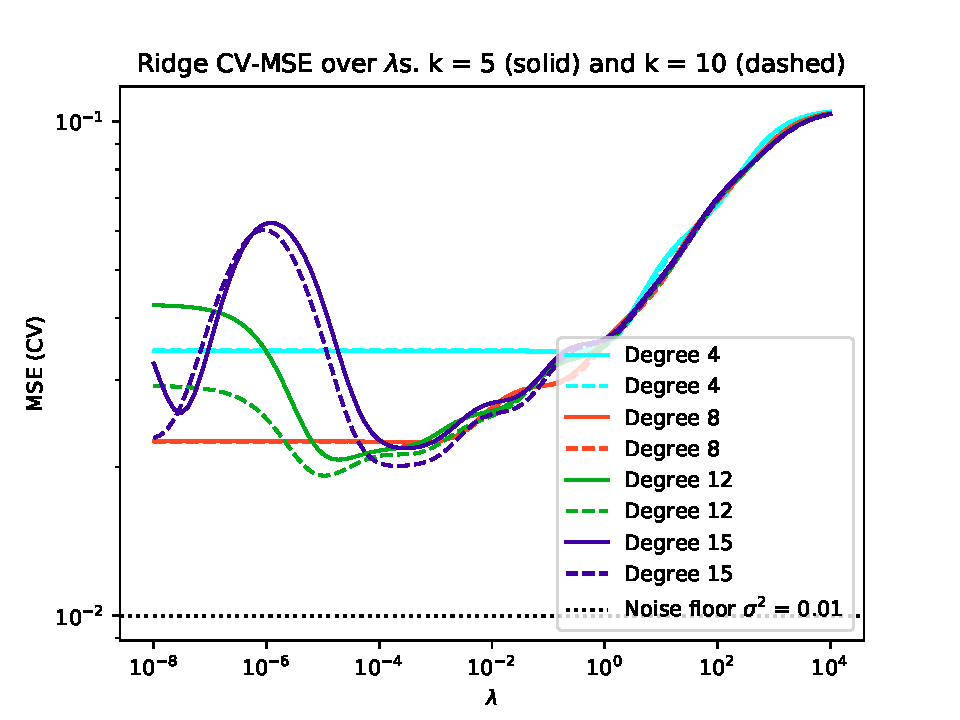
\includegraphics[width=\linewidth]{figs/Part_d_Ridge_k5_vs_k10_lambda.pdf}
    \caption{For low degrees the cross-validated MSE needs little to no regularisation and the curve is flat for low $\lambda$'s. When $\lambda$ increases all degrees converge to the same value}
    \label{fig:part_d_ridge_vs_lambdas}
\end{figure}


\subsection{Gradient descent code, with analytical gradients and automatic differentiation} % maria

For OLS and Ridge we find the difference between the optimal parameters $\bm{\theta}$, using the analytical expression and automatic differentiation. This confirms that our analytical gradient formula is correct. In table \ref{tab: Part e gradient_comparison}, the gradient differences are shown for both methods.\\
\begin{table}[h]
    \centering
    \begin{tabular}{l c}
        \toprule
         & $|\boldsymbol{\theta}_{\text{AD}} - \boldsymbol{\theta}_{\text{analytical}}|$ \\
        \midrule
        OLS   & $8.33 \times 10^{-16}$ \\
        Ridge & $8.33 \times 10^{-16}$ \\
        \bottomrule
    \end{tabular}
    \caption{Comparison of gradients (AD vs. analytical) for OLS and Ridge regression.}
    \label{tab: Part e gradient_comparison}
\end{table}\\
We want to find the best learning rate to use for our gradient descent. In figure \ref{fig: Part e error of gd with learningrate}, the solution of the gradient descent compared to the closed form solution is plotted as a function of the learning rate $\gamma$. The learning rate limit $\gamma_{\text{max}}$ is plotted for both OLS and Ridge, and we find that the limits are for OLS: $\gamma_{\text{max}} = 0.349$, and for Ridge: $\gamma_{\text{max}} = 0.348$. \\ 
To find the best learning rate, we plot the number of iterations required for the different learning rates, for the gradient descent solutions. In figure \ref{fig: Part e iteration vs learningrate}, we find the best learning rate $\gamma_{\text{best}}$ by finding the minimal number of iterations required, and we get $\gamma_{\text{best}} = 0.344$ for both methods. 
\begin{figure}[h!]
    \centering
    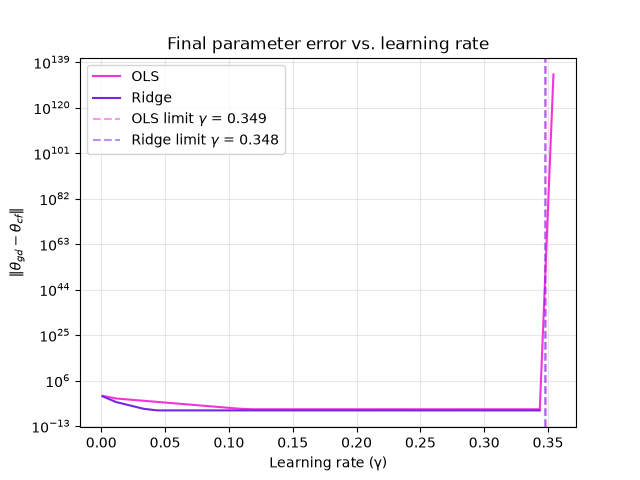
\includegraphics[width=\linewidth]{figs/Part_e_error_learningrate.png}
    \caption{The difference between the optimal parameter for the gradient descent solution and closed form solution as a function of the learning rate, for OLS and Ridge. The limit for the learning rate $\gamma_{\text{max}} = 0.349$ for OLS and $\gamma_{\text{max}} = 0.348$ for ridge. }
    \label{fig: Part e error of gd with learningrate}
\end{figure}
\begin{figure}[h!]
    \centering
    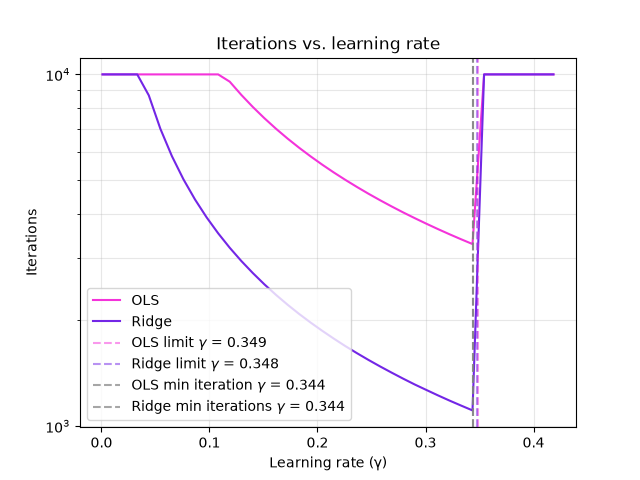
\includegraphics[width=\linewidth]{figs/Part_e_iteration_learningrate.png}
    \caption{Iterations as a function of the learning rate for OLS and Ridge. The learning rate that requires the least number of iterations is $\gamma_{\text{best}} = 0.344$ for both methods.}
    \label{fig: Part e iteration vs learningrate}
\end{figure}\\
We can find the difference between the analytical solution and the closed form solution, which tells us how close the gradient descent's final iterate gets to the optimal value. We do this for both $\gamma_{\text{max}}$ and $\gamma_{\text{best}}$. The results for these are found in table \ref{tab: Part e gradientdes_comparison}. In this table, the number of iterations it takes to find the optimal value is also shown. Note that for $\gamma_{\text{max}}$, the number of iterations it takes is $10\,000$, but this is also the number of iterations the program is set to. So it doesn't reach the optimal value within the set number of iteration, but rather the code has just reached its limit. \\
\begin{table}[h]
    \centering
    \begin{tabular}{l c c c c}
        \toprule
         & \multicolumn{2}{c}{$|\boldsymbol{\theta}_{\text{gd}} - \boldsymbol{\theta}_{\text{closed form}}|$} & \multicolumn{2}{c}{Iterations to converge} \\
        \cmidrule(lr){2-3} \cmidrule(lr){4-5}
         & $\gamma_{\text{max}}$ & $\gamma_{\text{best}}$ & $\gamma_{\text{max}}$ & $\gamma_{\text{best}}$ \\
        \midrule
        OLS   & $1.858 \times 10^{-2}$ & $7.718 \times 10^{-7}$ & $10\,000$ & $3293$ \\
        Ridge & $1.852 \times 10^{-2}$ & $2.581 \times 10^{-7}$ & $10\,000$ & $1108$ \\
        \bottomrule
    \end{tabular}
    \caption{Comparison of gradient descent for the closed form and analytical solution, for the learning rate limit $\gamma_{\text{max}}$ and the best learning rate $\gamma_{\text{best}}$.}
    \label{tab: Part e gradientdes_comparison}
\end{table}\\
We can further study the number of iterations required to reach the optimal value for different values of the learning rate, and in figure \ref{fig: Part e convergence} we do exactly this. \\
\begin{figure}[h!]
    \centering
    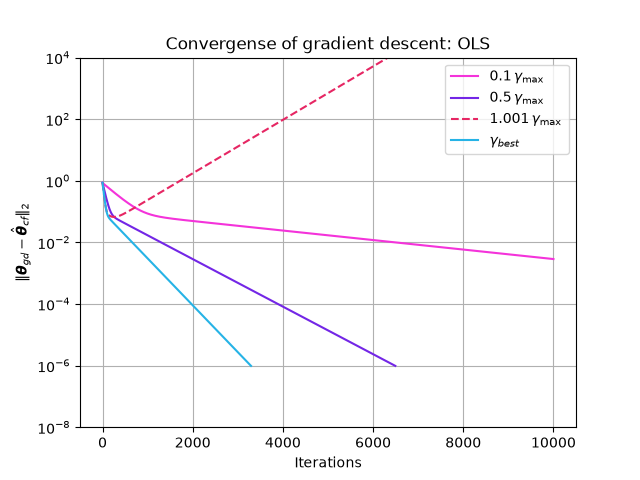
\includegraphics[width=\linewidth]{figs/Part_e_convergence_learningrate_OLS.png}
    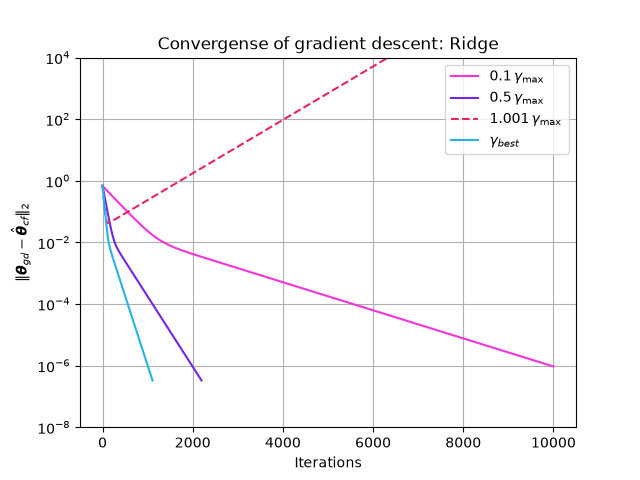
\includegraphics[width=\linewidth]{figs/Part_e_convergence_learningrate_Ridge.png}
    \caption{Convergence of the gradient descent method for OLS and Ridge, for different values of the learning rate $\gamma$. For a learning rate larger than $\gamma_{\text{max}}$, the solution diverges. }
    \label{fig: Part e convergence}
\end{figure}
When we've now found the best value for the learning rate, we can use this to study the cost function of the different methods. In figure \ref{fig: Part e cost ols vs ridge}, we've done this for both $\gamma_{\text{max}}$ and $\gamma_{\text{best}}$. \\ 
\begin{figure}[h!]
    \centering
    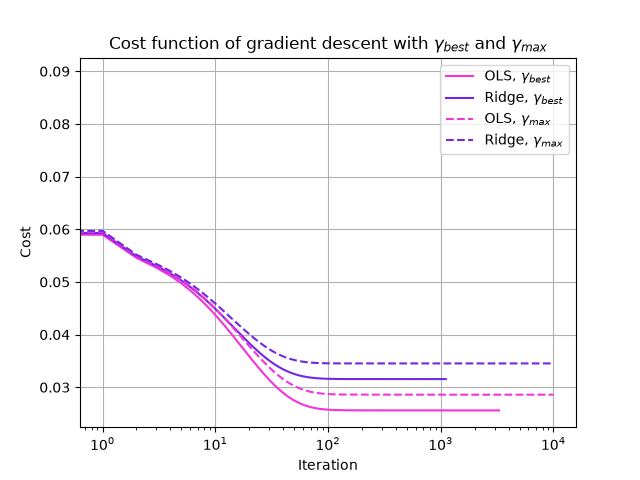
\includegraphics[width=\linewidth]{figs/Part_e_costfunc_OLS_Ridge.png}
    \caption{Cost function of OLS and Ridge as a function of number of iterations. The solution with the best learning rate converges faster. Values of the final cost and iterations is shown in table \ref{tab: Part e gradientdes_comparison}.}
    \label{fig: Part e cost ols vs ridge}
\end{figure}
We've now trained the gradient descent method on the data we set aside, but how well does it hold up when tested?
In figure \ref{fig: Part e test train hist ridge ols}, the MSE of the test data is compared to the training data. \\
\begin{figure}[h!]
    \centering
    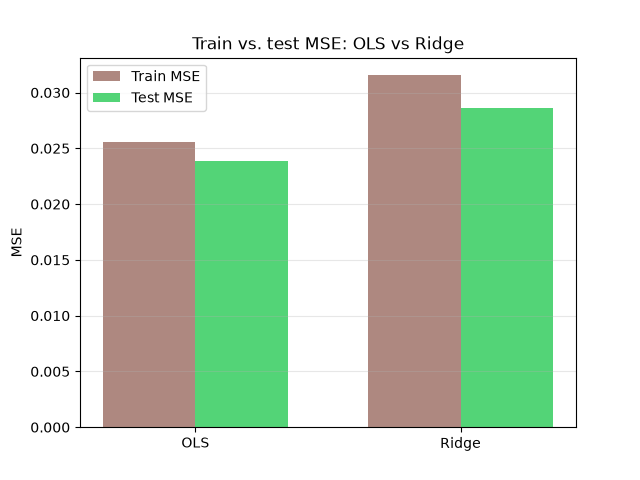
\includegraphics[width=\linewidth]{figs/Part_e_hist_testtrain.png}
    \caption{Comparing the MSE of the test and training data for OLS and Ridge.}
    \label{fig: Part e test train hist ridge ols}
\end{figure}
For Ridge, where there is a penalty $\lambda$, and we can study how this penalty effects the MSE of the training data and compare to the MSE of the test data. This has been plotted in figure \ref{fig: Part e test train ridge}. 
\begin{figure}[h!]
    \centering
    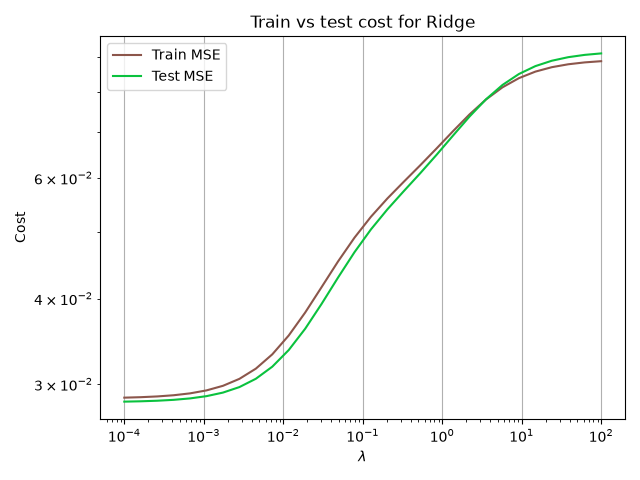
\includegraphics[width=\linewidth]{figs/Part_e_cost_lambda_testtrain.png}
    \caption{The MSE of the training and test data as a function of the penalty factor $\lambda$, for Ridge.}
    \label{fig: Part e test train ridge}
\end{figure}

\clearpage 
\subsection{Including momentum and more advanced ways to update the learning rate} % hannah

The gradient descent methods Plain Gradient Descent (\textbf{PGD}), Momentum, AdaGrad, RMSProp and Adam have a varied number of needed iterations for convergence to have excess cost be reduced below the tolerance. In \cref{fig:GDmethods_iterations} we see that for a tolerance of $10^{-4}$ all models eventually converge for some learning rates. The number of iterations needed to so change drastically, but trend towards less needed iterations as learning rate and hence the step size increases. Neither AdaGrad nor PGD manage to converge for learning rates close to $2/\lambda_\text{max}$. Momentum fails to converge above $2(1+\beta)/\lambda_\text{max}$, which is seen as the limit for the method's convergence. 

When we decrease the tolerance to $10^{-8}$, the possible learning rates for convergence decreases drastically. RMSProp fails to converge for any rate, and plain gradient descent has a severely limited learning rate range. We see that for large rates, Momentum converges the fastest, but over all Adam does reasonably well for all rates, converging at only ~200 iterations more than Momentum does at its best. For learning rates above momentums limit, it does not converge, but both PGD and Adam does, although PGD's $\gamma_\text{max}$ should be surpassed. 

\begin{figure}[h!]
    \centering
    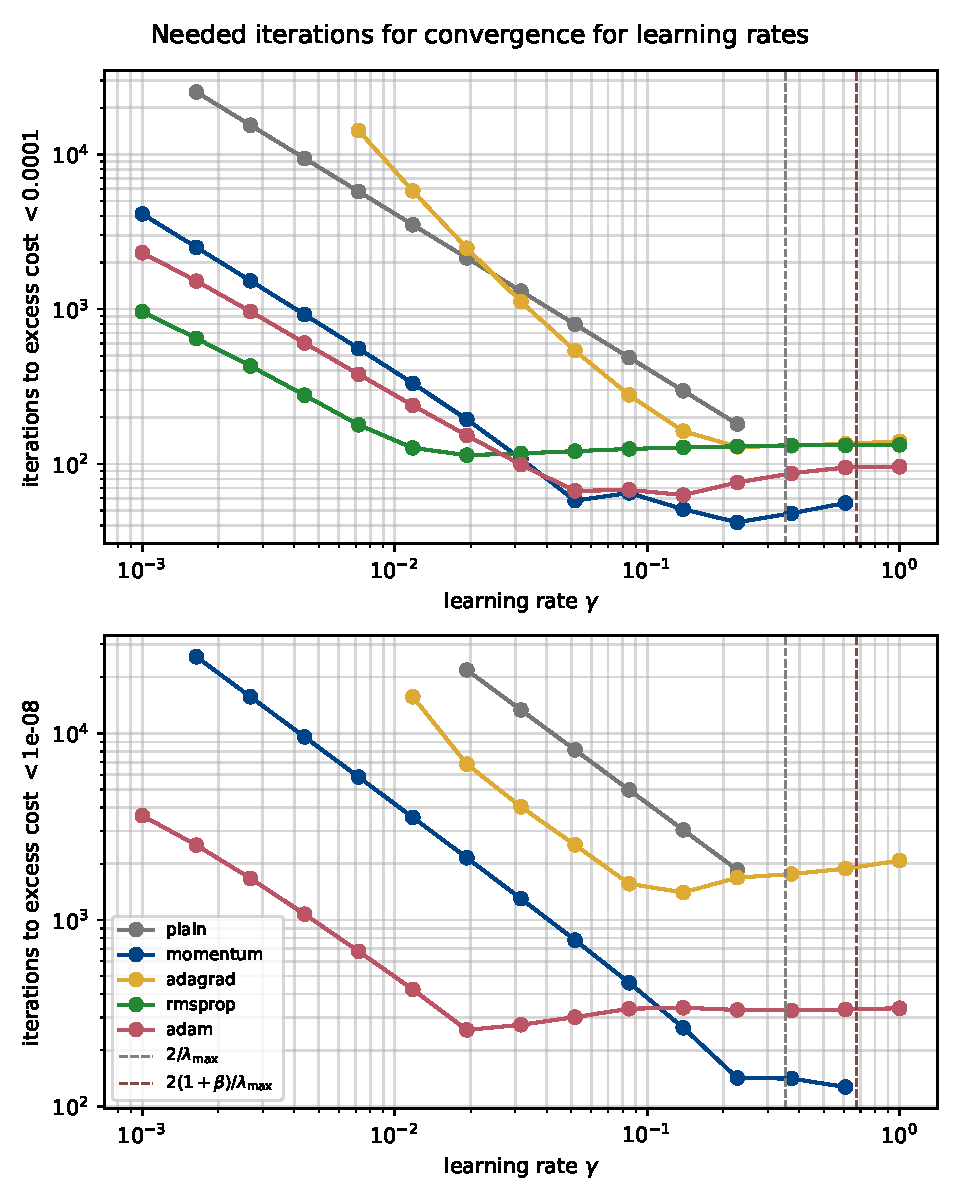
\includegraphics[width=1\linewidth]{figs/Part_f_MethodsComparison_withLearningRate.pdf}
    \caption{The various models have different ranges of learning rate $\gamma$ that allows the cost version to converge.}
    \label{fig:GDmethods_iterations}
\end{figure}


\subsection{Lasso regression} % maria
Before comparing the different Lasso solvers, we first check why \texttt{lasso\_gd} uses an explicit sub gradient rule rather than letting JAX differentiate the $\ell_1$ penalty automatically. The $\ell_1$ term $|\theta|$ is not differentiable at $\theta = 0$, so its true derivative there is only defined as a sub gradient, any value in $[-1, 1]$. Table \ref{tab: Part g AD subgradient} shows what JAX's automatic differentiation (AD) returns at $\theta = 0$ and at nearby points. 
\begin{table}[h]
    \centering
    \begin{tabular}{c c}
        \toprule
        $\theta$ & $d|\theta|/d\theta$ (JAX AD) \\
        \midrule
        $-1.0 \times 10^{-3}$ & $-1.0$ \\
        $-1.0 \times 10^{-9}$ & $-1.0$ \\
        $0.0$                 & $+1.0$ \\
        $1.0 \times 10^{-9}$  & $+1.0$ \\
        $1.0 \times 10^{-3}$  & $+1.0$ \\
        \bottomrule
    \end{tabular}
    \caption{Automatic differentiation (JAX) derivative of $|\theta|$ at $\theta = 0$ and nearby points. At $\theta = 0$, JAX returns $+1.0$ rather than the true sub gradient interval $[-1, 1]$ or a value consistent with the sign of nearby points — an artefact of how \texttt{jnp.abs} is implemented, not a principled sub gradient choice.}
    \label{tab: Part g AD subgradient}
\end{table}\\
We've now also implemented the method Lasso regression and will compare to OLS and Ridge. Since Lasso doesn't have a closed form solution for us to compare to, we've instead compared different way of doing a Lasso regression to each other. \\
In table \ref{tab: Part g lasso comparison} we compare the SciKit Learn package \cite{SKlearn_lasso} to the gradient descent and coordinate descent methods, and we look at the number of iterations it takes to reach the optimal values. \\ 
\begin{table}[h]
    \centering
    \begin{tabular}{l c c}
        \toprule
        \textbf{Method} & Iterations to converge & $|\boldsymbol{\theta} - \boldsymbol{\theta}_{\text{sklearn}}|$ \\
        \midrule
        Scikit-learn        & 307 & --- \\
        Gradient descent    & 513 & $2.46 \times 10^{-7}$ \\
        Coordinate descent  & 181 & $1.06 \times 10^{-7}$ \\
        \bottomrule
    \end{tabular}
    \caption{Comparison of Lasso solvers: number of iterations to converge, and maximum absolute deviation from the scikit-learn reference solution.}
    \label{tab: Part g lasso comparison}
\end{table}\\

We now need to compare Lasso to OLS and Ridge, in figure \ref{fig: Part g cost func} we have compared the cost functions of OLS, Ridge and Lasso for both gradient and coordinate descent. \\
\begin{figure}[h!]
    \centering
    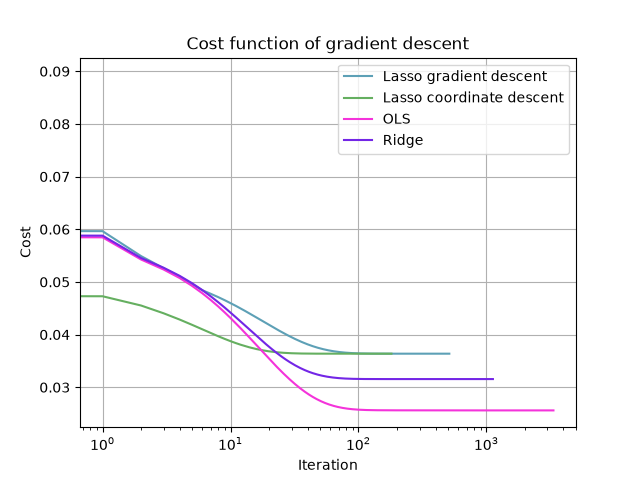
\includegraphics[width=\linewidth]{figs/Part_g_convergence_Lasso.png}
    \caption{Cost function for OLS, Ridge and Lasso for Gradient descent and Coordinate descent. Values for iterations and final cost for the two Lasso methods is found in table \ref{tab: Part g lasso comparison}.}
    \label{fig: Part g cost func}
\end{figure}\\
\begin{table}[h!]
    \centering
    \begin{tabular}{l c c}
        \toprule
        \textbf{Method} & Train & Test \\
        \midrule
        OLS  & $2.561 \times 10^{-2}$ & $2.390 \times 10^{-2}$ \\
        Ridge    & $2.677 \times 10^{-2}$ & $2.382 \times 10^{-2}$ \\
        Lasso  & $2.688 \times 10^{-2}$ & $2.381 \times 10^{-2}$ \\
        \bottomrule
    \end{tabular}
    \caption{Train and test MSE for OLS, Ridge and Lasso}
    \label{tab: Part g train test}
\end{table}\\
We also need to see how Lasso regression holds up when we test it on the data the model hasn't been trained on. We extend the OLS/Ridge comparison of figure \ref{fig: Part e test train hist ridge ols} by adding Lasso, shown in figure \ref{fig: Part g hist lasso} \\
\begin{figure}[h!]
    \centering
    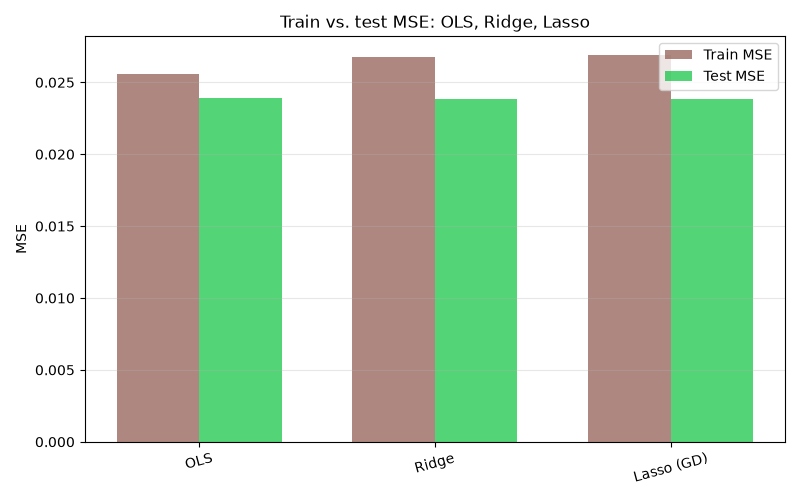
\includegraphics[width=\linewidth]{figs/Part_g_hist_testtrain_lasso.png}
    \caption{Comparing the MSE of the test and training data for OLS, Ridge and Lasso. Values for different MSE are found in table \ref{tab: Part g train test}.}
    \label{fig: Part g hist lasso}
\end{figure}\\
Since we also have a penalty factor $\lambda$ for Lasso regression, we can again look at how $\lambda$ effects the MSE for the training and test data. In figure \ref{fig: Part g train test lasso}, the MSE for Lasso and Ridge is plotted to compare how well the model works on the test data. \\
\begin{figure}[h!]
    \centering
    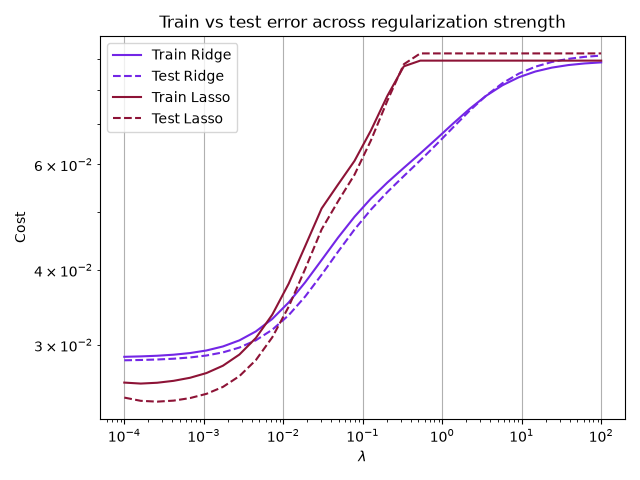
\includegraphics[width=\linewidth]{figs/Part_g_cost_lambda_testtrain.png}
    \caption{The MSE of the training and test data as a function of the penalty factor $\lambda$, for Ridge and Lasso.}
    \label{fig: Part g train test lasso}
\end{figure}
Figure \ref{fig: Part g theta_lambda} shows how the individual coefficients of Ridge and Lasso shrink as $\lambda$ increases. For Ridge, all coefficients shrink smoothly and continuously toward zero as $\lambda$ grows, but none of them reach exactly zero. Lasso instead drives coefficients to exactly zero one at a time as $\lambda$ increases, performing implicit feature selection rather than just shrinkage. This matches what we see at $\lambda = 10^{-2}$ specifically: scikit-learn's Lasso solution is $\boldsymbol{\theta} = [0, -0.569, 0, 0.381, 0]$, with three of the five coefficients set exactly to zero, while the corresponding Ridge solution at the same $\lambda$ has no zero entries at all, with the solution being $\boldsymbol{\theta} = [-0.005, -0.574, 0.015, 0.387, -0.012]$.
\begin{figure}[h!]
    \centering
    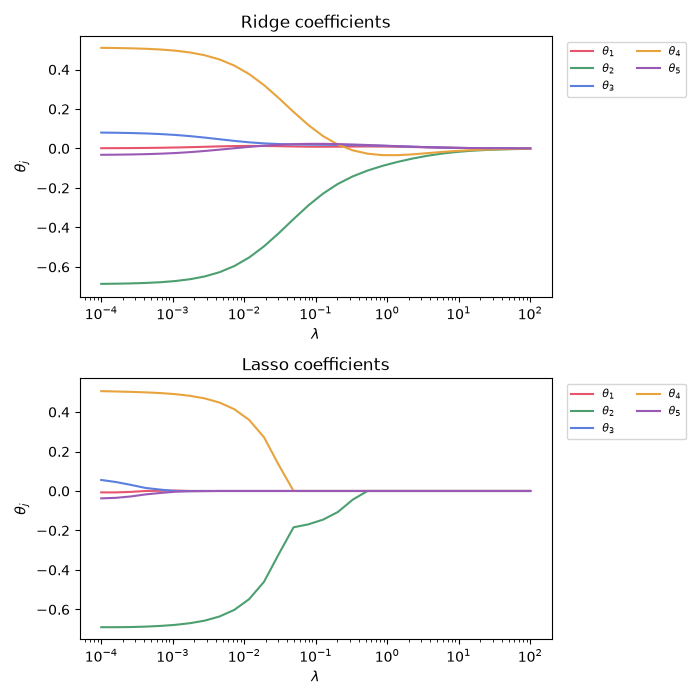
\includegraphics[width=\linewidth]{figs/Part_g_theta_lambda.png}
    \caption{The coefficients for Ridge and Lasso as a function of penalty $\lambda$. For smaller penalty values, the coefficients are large, and for ridge they shrink toward zero as the penalty increases. For Lasso they are put to exactly zero one after the other.  }
    \label{fig: Part g theta_lambda}
\end{figure}

\subsection{Stochastic gradient descent} % maria
For the Stochastic Gradient Descent (SGD) method, there are multiple parameters we can change, and thereafter study the effect of. Firstly we study what happens when the batch size is changed, but the number of batches is held constant. In figure \ref{fig: Part h batch size}, this is plotted for three different batch sizes. In figure \ref{fig: Part h batchsize heatmap} we have plotted a heat map of the varying batch size in order to show how the cost is effected for a range of batch sizes. \\
\begin{figure}[h!]
    \centering
    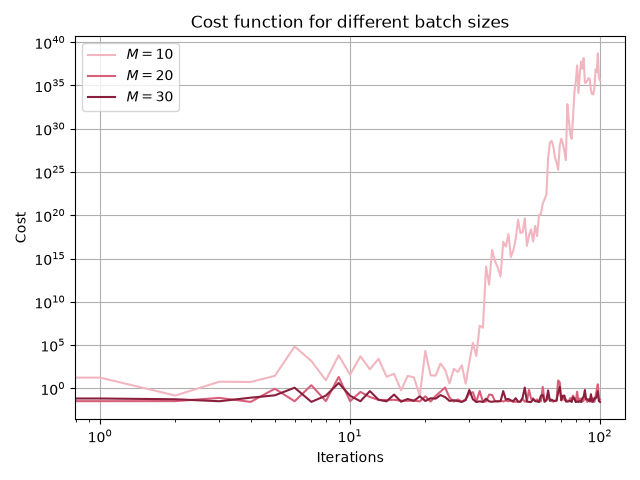
\includegraphics[width=\linewidth]{figs/Part_h_cost_batchsize.png}
    \caption{Cost function for SGD for different batch sizes $M$. For $M = 10$, the cost increases by a lot more than for larger batch sizes. }
    \label{fig: Part h batch size}
\end{figure}
\begin{figure}[h!]
    \centering
    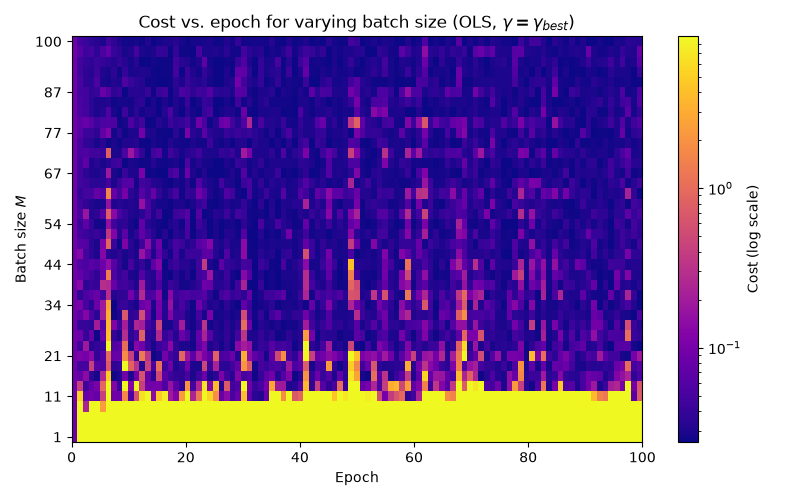
\includegraphics[width=\linewidth]{figs/Part_h_heatmap_batchsize.png}
    \caption{Cost function for SGD for different batch sizes $M$.}
    \label{fig: Part h batchsize heatmap}
\end{figure}\\
Next, in figure \ref{fig: Part h learningrate}, we change the learning rate and plot the cost function for these different learning rates. In figure \ref{fig: Part h learningrate heatmap}, we have plotted a heat map of the varying learning rate. \\  
\begin{figure}[h!]
    \centering
    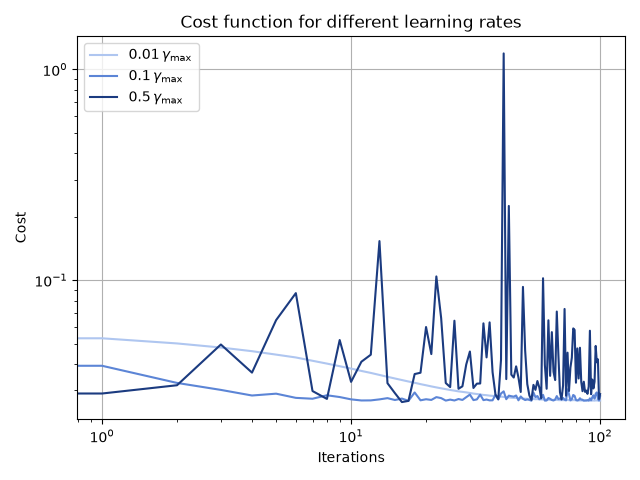
\includegraphics[width=\linewidth]{figs/Part_h_cost_learningrates.png}
    \caption{Cost function for SGD for different learning rates $\gamma$. For a learning rate of $0.5 \, \gamma_{\text{max}}$, cost starts to become unstable.}
    \label{fig: Part h learningrate}
\end{figure}
\begin{figure}[h!]
    \centering
    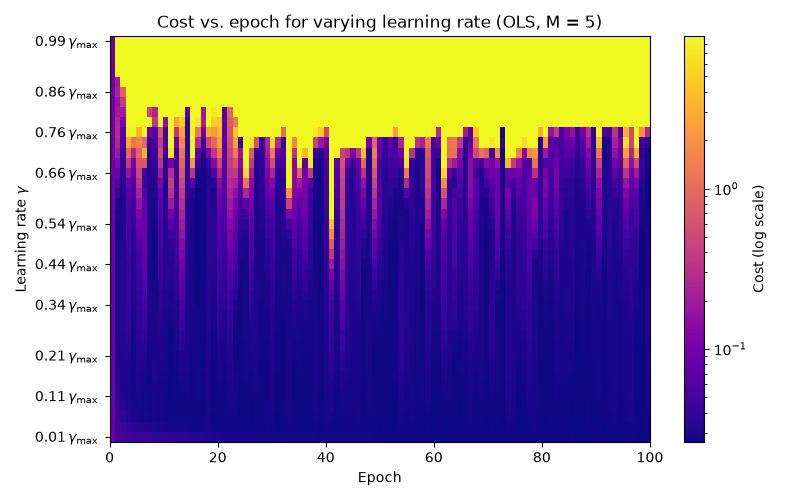
\includegraphics[width=\linewidth]{figs/Part_h_heatmap_learningrate.png}
    \caption{Cost function for SGD for different learning rates $\gamma$.}
    \label{fig: Part h learningrate heatmap}
\end{figure}\\
In figure \ref{fig: Part h schedule} we use the decaying schedule, given in equation \ref{eq: decaying schedule}, to show the cost function for OLS. 
\begin{figure}[h!]
    \centering
    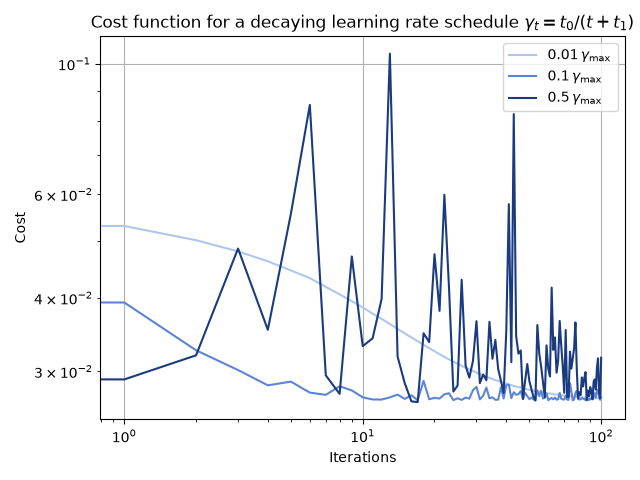
\includegraphics[width=\linewidth]{figs/Part_h_cost_schedule.png}
    \caption{Cost function for SGD with a decaying learning rate schedule $\gamma_t = t_0/(t+t_1)$, for three initial rates matching those of figure \ref{fig: Part h learningrate}. Cost here is generally lower than in figure \ref{fig: Part h learningrate}.}
    \label{fig: Part h schedule}
\end{figure}
We then compare the schedule directly against holding $\gamma$ constant at the same initial values, shown in figure \ref{fig: Part h schedule vs constant}. Since the two cost functions are relatively similar, we have also shown the difference between the in this figure, as well as the actual learning rate that is used for the two methods. With $t_1$ chosen relative to the total number of iteration the program performs, the schedule reaches within 1 \% the closed form solution in the same number of iterations as when the learning rate is held constant: 480 iterations. The parameters ended with $|\theta_{\text{schedule}} - \theta_{\text{constant}}| = 1.28\times10^{-2}$, for the two methods.\\
We compare plain SGD with the four adaptive optimiser: momentum, Adagrad, RMSprop and Adam, for both OLS and Ridge, as shown in figure \ref{fig: Part h optimiser comparison}. Table \ref{tab: Part h optimiser comparison} reports, for each method, the number of iterations needed to reach within 1\% of the closed-form cost, and the final distance to the closed-form solution.
\begin{table}[h!]
\centering
    \begin{tabular}{l c c|c | c|c}
        \hline
        & & \multicolumn{2}{c}{OLS} & \multicolumn{2}{c}{Ridge} \\
        \cline{3-4} \cline{5-6}
        Optimiser & $\gamma$ & Iter. & $|\theta-\theta_{\text{cf}}|$ & Iter. & $|\theta-\theta_{\text{cf}}|$ \\
        \hline
        Plain SGD & 0.1  & 2720 & $3.71\times10^{-2}$ & 3840 & $2.87\times10^{-2}$ \\
        Momentum  & 0.01 & 6240 & $2.39\times10^{-2}$ & 1120 & $2.29\times10^{-2}$ \\
        Adagrad   & 0.1  & 1760 & $2.71\times10^{-2}$ & 1120 & $1.52\times10^{-3}$ \\
        RMSprop   & 0.1  & 6240 & $1.95\times10^{-1}$ & n/a  & $1.54\times10^{-1}$ \\
        Adam      & 0.1  & 4640 & $6.06\times10^{-2}$ & n/a  & $8.94\times10^{-2}$ \\
        \hline
    \end{tabular}
    \caption{Comparison of SGD optimisers for OLS and Ridge: iterations needed to reach within 1\% of the closed-form cost (out of 8000 total updates run), and the final distance to the closed-form solution.}
\label{tab: Part h optimiser comparison}
\end{table}\\

We can also compare SGD to standard gradient descent, and see how they compare to each other. In figure \ref{fig: Part h cost func}, we compare the two models, and table \ref{tab: Part h gd sgd iterations} reports the number of iterations each took to converge and the resulting distance between their solutions. \\
\begin{figure}[h!]
    \centering
    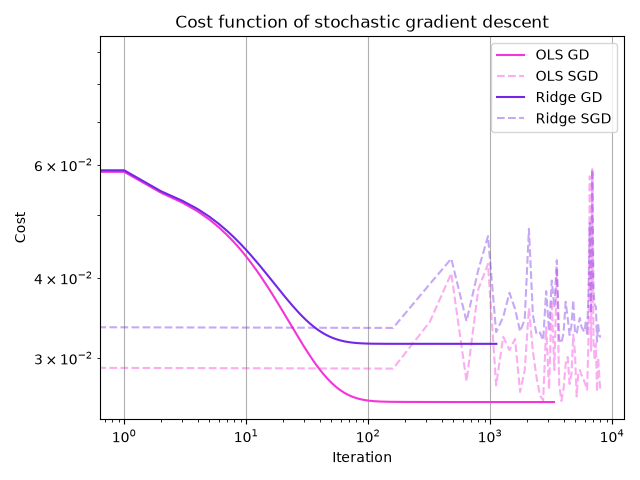
\includegraphics[width=\linewidth]{figs/Part_h_sgd_OLS_Ridge.png}
    \caption{Cost function for OLS and Ridge using gradient descent and stochastic gradient descent. Difference between final values of cost and iterations to converge are shown in table \ref{tab: Part h gd sgd iterations}.}
    \label{fig: Part h cost func}
\end{figure}

\begin{table}[h!]
\centering
    \begin{tabular}{l c c c}
        \hline
        Method & GD iter. & SGD iter. & $|\theta_{\text{SGD}} - \theta_{\text{GD}}|$ \\
        \hline
        OLS   & 3341 & 8001 & $3.71\times10^{-2}$ \\
        Ridge & 1124 & 8001 & $2.87\times10^{-2}$ \\
        \hline
    \end{tabular}
    \caption{Iterations to converge for gradient descent (GD) and stochastic gradient descent (SGD), for OLS and Ridge regression.}
    \label{tab: Part h gd sgd iterations}
\end{table}

We also need to study how this model holds up when tested, just as we did for gradient descent. In figure \ref{fig: Part h hist test}, the MSE for the training and test data is shown for OLS and Ridge, for both GD and SGD, with the exact values reported in table \ref{tab: Part h traintest mse}.  
\begin{figure}[h!]
    \centering
    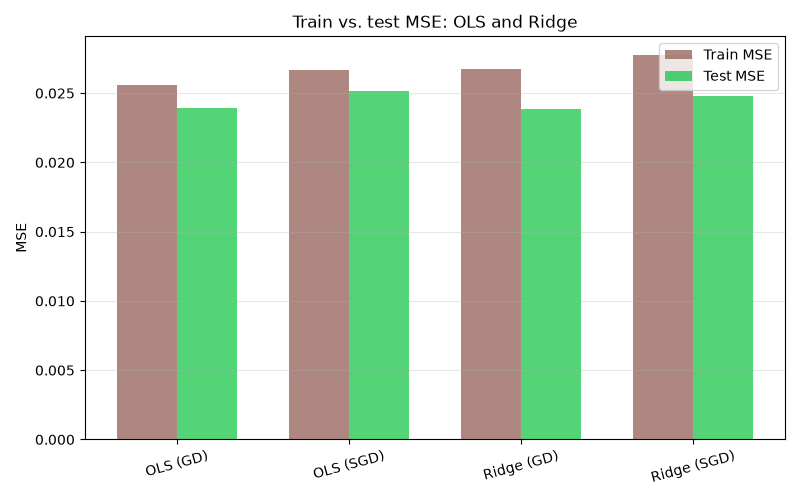
\includegraphics[width=\linewidth]{figs/Part_h_hist_testtrain_sgd.png}
    \caption{Train and test MSE for OLS and Ridge, via gradient descent (GD) and stochastic gradient descent (SGD). Values for the different MSE are found in table \ref{tab: Part h traintest mse}.}
    \label{fig: Part h hist test}
\end{figure}
\begin{table}[h!]
    \centering
    \begin{tabular}{l c c c}
        \hline
        Method & Train MSE & Test MSE & Gap (test $-$ train) \\
        \hline
        OLS (GD)    & $2.5608\times10^{-2}$ & $2.3899\times10^{-2}$ & $-1.7087\times10^{-3}$ \\
        OLS (SGD)   & $2.6703\times10^{-2}$ & $2.5164\times10^{-2}$ & $-1.5394\times10^{-3}$ \\
        Ridge (GD)  & $2.6765\times10^{-2}$ & $2.3821\times10^{-2}$ & $-2.9446\times10^{-3}$ \\
        Ridge (SGD) & $2.7738\times10^{-2}$ & $2.4792\times10^{-2}$ & $-2.9462\times10^{-3}$ \\
        \hline
    \end{tabular}
    \caption{Train and test MSE for OLS and Ridge, via gradient descent (GD) and stochastic gradient descent (SGD).}
    \label{tab: Part h traintest mse}
\end{table}

\begin{figure*}[h!]
    \centering
    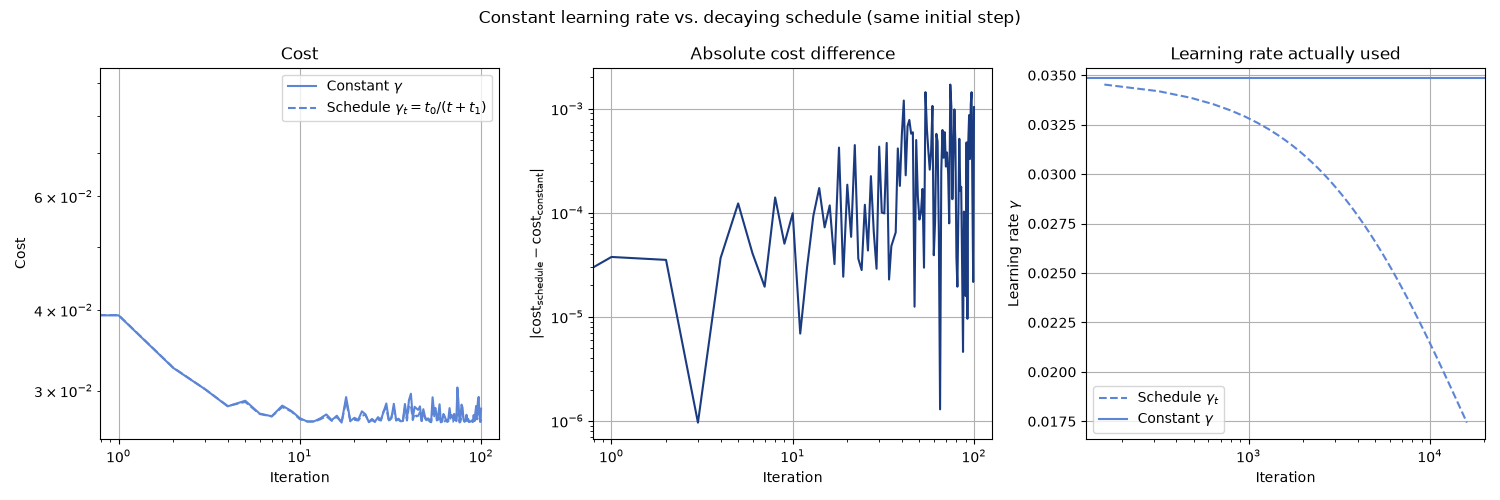
\includegraphics[width=\textwidth]{figs/Part_h_schedule_vs_constant.png}
    \caption{Left: cost function for SGD with a constant learning rate versus a decaying schedule with the same initial step, for OLS. Middle: absolute difference between the two cost curves. Right: the learning rate each method actually used at each iteration.}
    \label{fig: Part h schedule vs constant}
\end{figure*}
\begin{figure*}[h!]
    \centering
    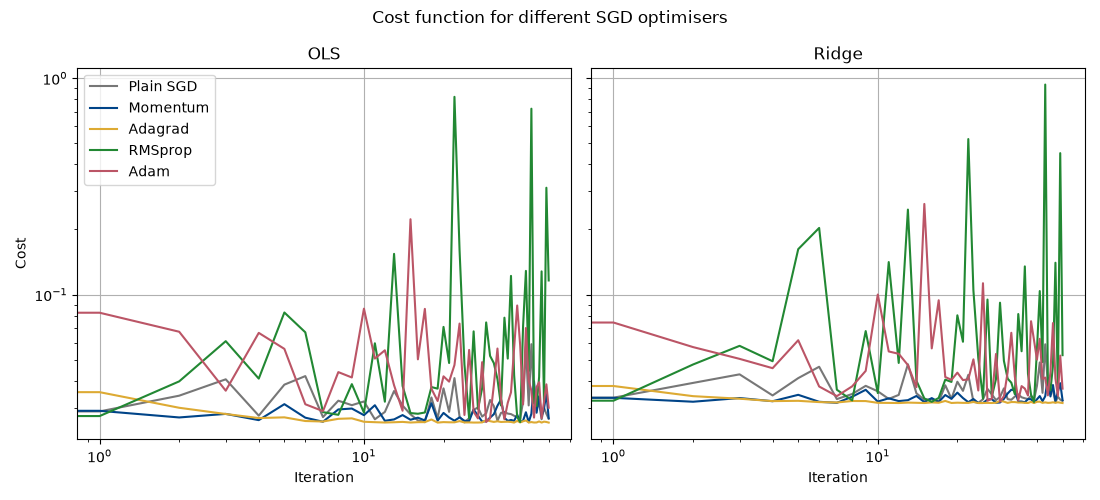
\includegraphics[width=\textwidth]{figs/Part_h_optimizer_comparison.png}
    \caption{Cost function for SGD with plain, momentum, Adagrad, RMSprop and Adam optimisers, for OLS (on the left) and Ridge (on the right). Cost is generally higher for Ridge.}
    \label{fig: Part h optimiser comparison}
\end{figure*}

\clearpage

\subsection{Cross-validation with hyperparameters} % hannah
With the k-fold cross-validation method implemented as in \ref{sec:cv-second-implementation}, we see how the MSE changes for the degrees \cref{fig:Part_i_MSE_testandtrain}. For the Ridge and Lasso estimators, the best scores range between $10^{-1}$ and $10^{-2}$ for both folds 5 and 10. Their MSEs vary somewhat from degree to degree, but remain mostly stable. Note that the Ridge test and train MSEs are the closest for their respective best scores. 

The OLS with 5 and 10 folds tells a different story, with its only tunable parameter being number of degrees. At best, the MSE is $2.5\times10^{-2}$ at the 8th degree, but blows up the order of $10^{2}$ for higher polynomials.

The best tuned models have different best penalties $\lambda$ as shown in\cref{fig:Part_i_besthyperparameters}. Ridge penalties for both fold follow the same trend, and the same goes for Lasso. This is expected behaviour as per their mathematical descriptions. In both cases, the best $\lambda$ follow a rough valley shape.


\begin{figure}
    \centering
    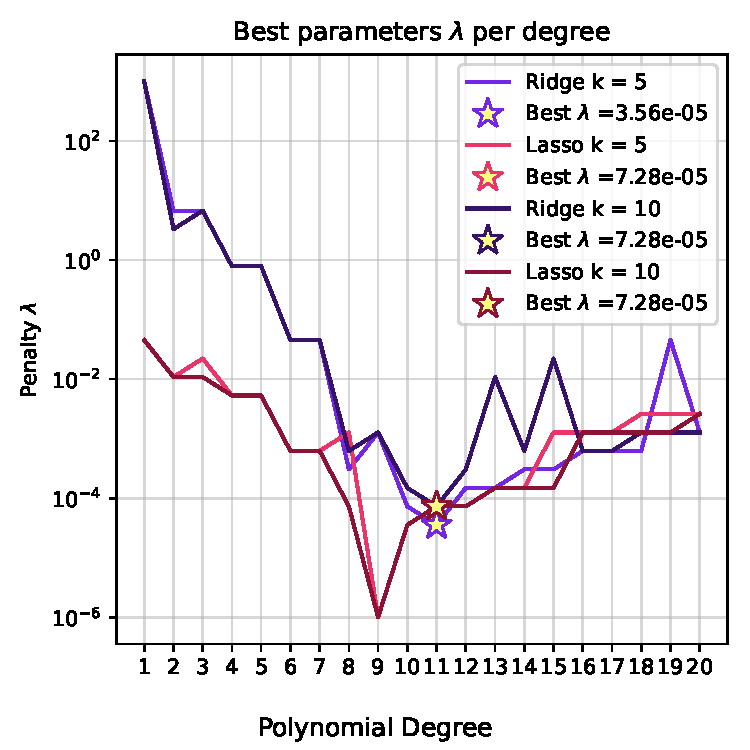
\includegraphics[width=0.8\linewidth]{figs/Part_i_besthyperparameters.pdf}
    \caption{The penalty $\lambda$ is shown for each degree per by their minimised cost functions as in \cref{fig:Part_i_MSE_testandtrain}. The $\lambda$ varies for the models, but are all on the same order of magnitude for the degree and chosen.}
    \label{fig:Part_i_besthyperparameters}
\end{figure}

\begin{figure}
    \centering
    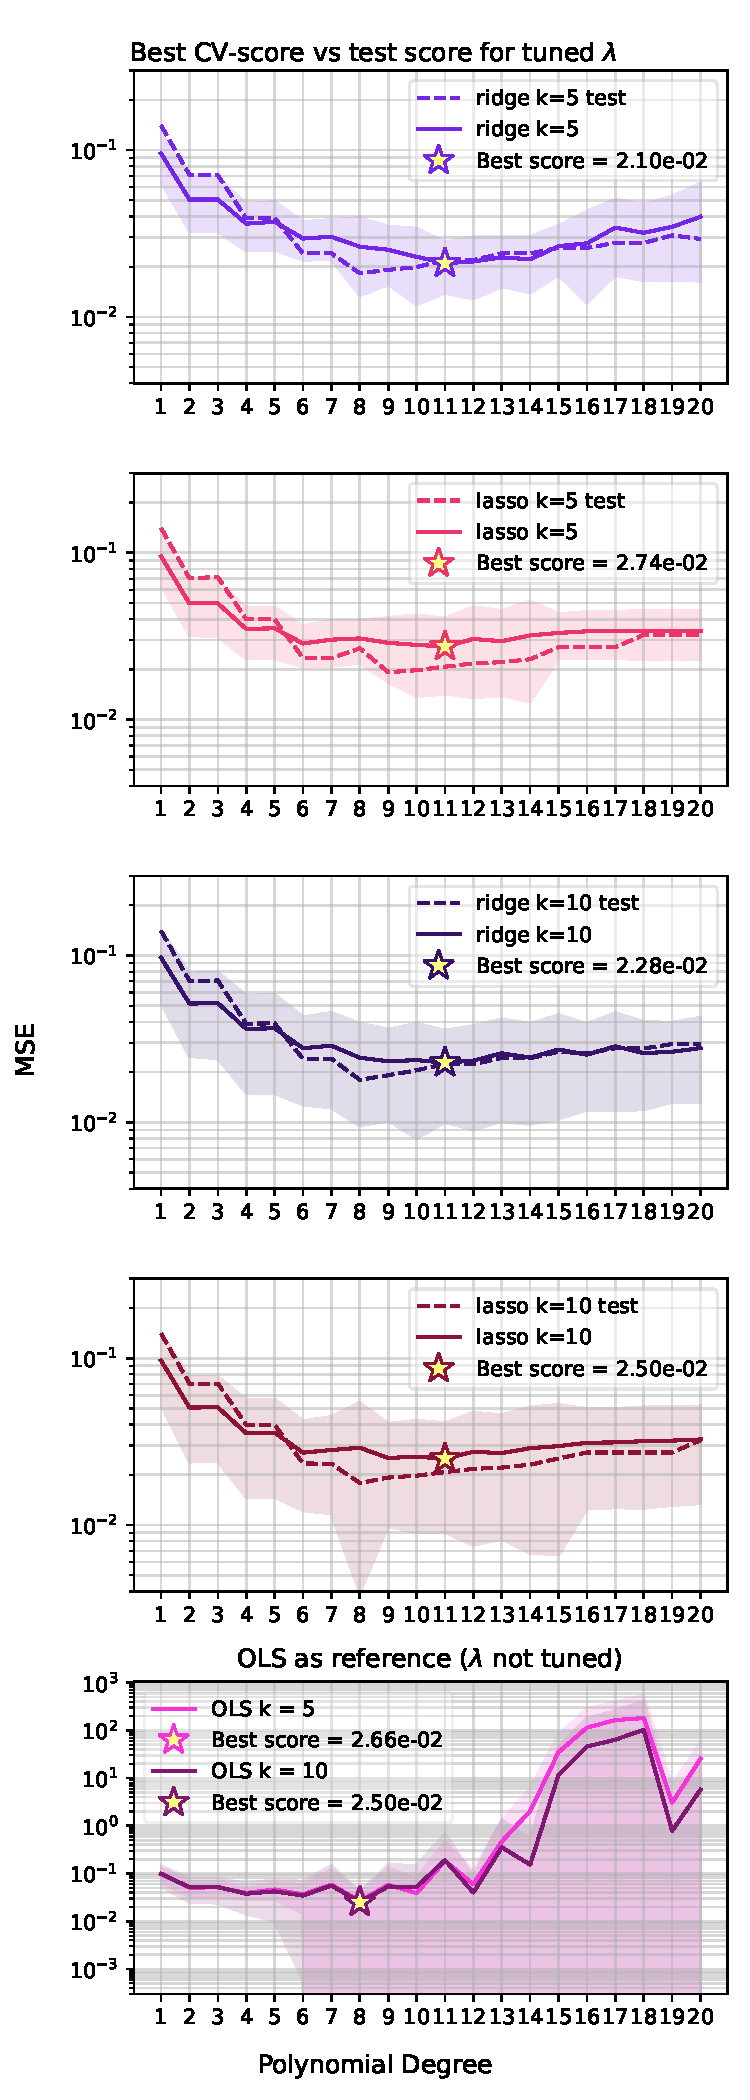
\includegraphics[width=0.85\linewidth]{figs/Part_i_MSE_testandtrain.pdf}
    \caption{As a combination of both degree and penalty $\lambda$, the minimised cost function per best combination is shown. Standard deviation for the train MSEs are included. See \cref{fig:Part_i_besthyperparameters} for penalty per degree. F degrees 6 and onwards for Ridge and Lasso the MSE remains on the same order of magnitude. Note that OLS is only used as a reference. For all fold sizes and estimators Ridge and Lambda the best score occurs at the 11th degree.}
    \label{fig:Part_i_MSE_testandtrain}
\end{figure}

The best estimators were attempted to be decomposed following \cref{sec:bootstrap}, but with data limited to the training set. The result is a poor decomposition for higher degrees(\cref{fig:Part_i_hyperparameters_msedecomposition_kfold_bootstrap}), where the error, which is the bootstrap MSE, in no way reflects the training MSE. We This is especially clear for the Ridge MSE decomposition. 
As for below 7 degrees we manage to decompose the MSE reasonably well with both resampling strategies, though the variance of the bootstrap and k-fold resampling can differ by a factor of 5. While size might differ, they yield a similar slopes. In both resampling methods for all folds and estimators, the bias is the most significant contributor.
In the appendix in \cref{fig:apdx:MSE_decomposition} there is a MSE decomposition for 5 fold Ridge with the whole dataset compared to the train dataset only. When the full dataset is used, the error is similar to the test and train MSEs. In all cases the bias contributes the most to the error, but variance plays a bigger part as the degrees increase. 


\begin{figure}
    \centering
    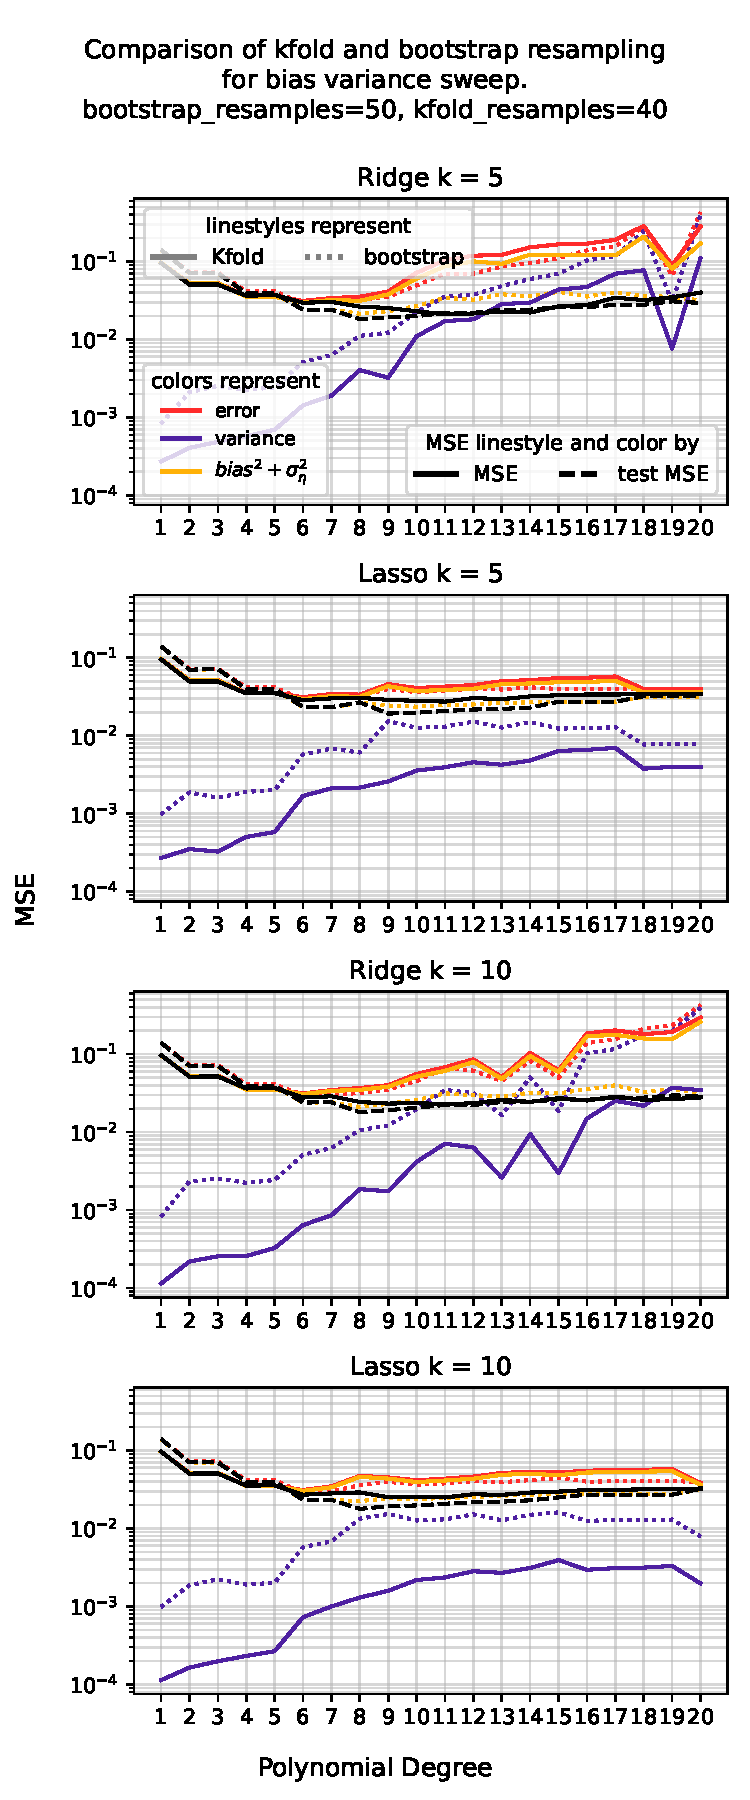
\includegraphics[width=0.8\linewidth]{figs/Part_i_hyperparameters_msedecomposition_kfold_bootstrap.pdf}
    \caption{Bootstrap and kfold resampling to decompose MSE. The error and MSE has the same mathemathical description \eqref{eq:MSE}, but uses the resampled data}
    \label{fig:Part_i_hyperparameters_msedecomposition_kfold_bootstrap}
\end{figure}

The with the best estimators for each fold refit to the whole training set, we get \cref{fig:Part_i_bestfits}. We see that all five models deviate from the Runge function, especially when the generated data is sparse. The 5- and 10-fold Lasso model does somewhat better, with the fit in the range of $x=-1.00$ and $x=-0.50$ much closer to the Runge function as opposed to Ridge models. 

\begin{figure}
    \centering
    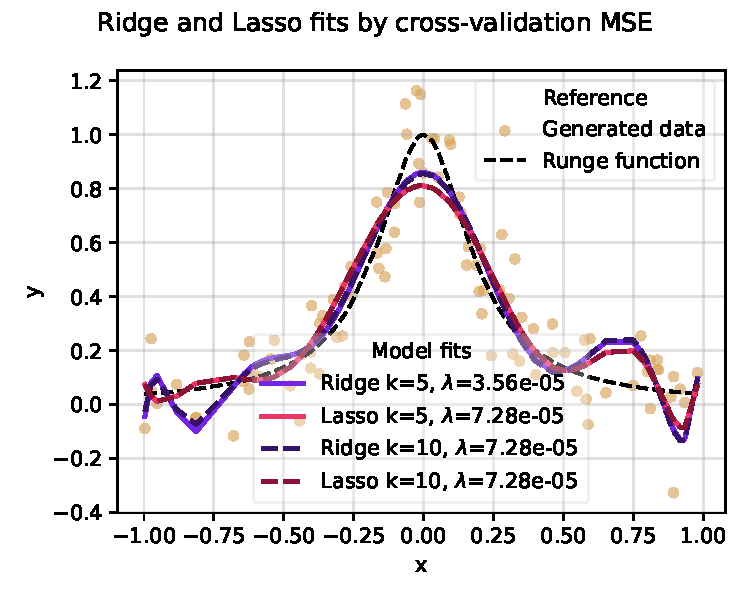
\includegraphics[width=1\linewidth]{figs/Part_i_best_fits.pdf}
    \caption{The fits of the estimators Ridge and Lasso with k=5,10 behave similarly, but deviate from the true Runge-function and generated data from it.}
    \label{fig:Part_i_bestfits}
\end{figure}

When we choose the cheapest permissible models instead as in \cref{fig:Part_i_setdegsfits}, we see that both Lasso models and the 5-fold Ridge model with their lower degrees (4 and 5) follow the curves worse than the 8 degree 5-fold Ridge fit. 

\begin{figure}
    \centering
    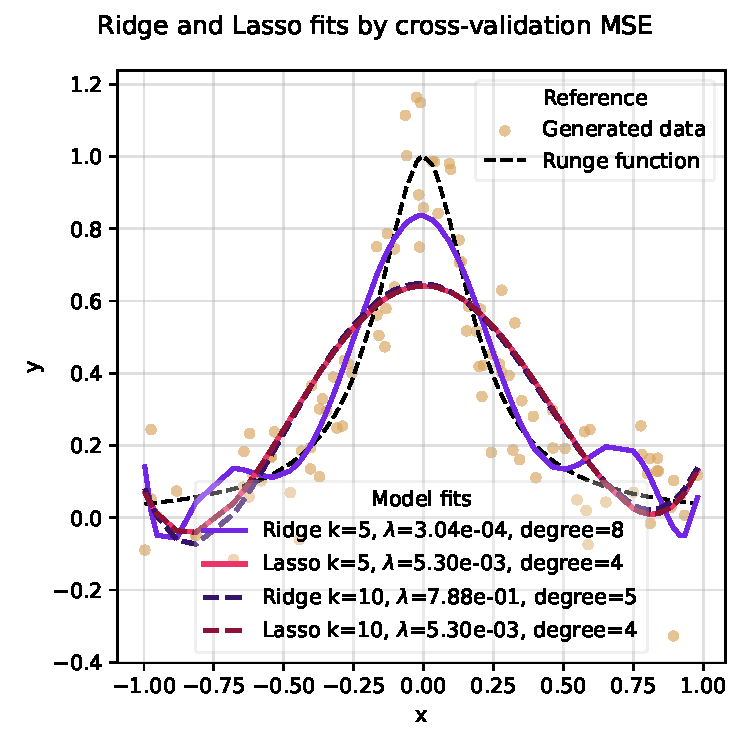
\includegraphics[width=0.8\linewidth]{figs/Part_i_setdegsfits.pdf}
    \caption{The cheapest fits with MSE within one standard deviation are chosen, showing how r }
    \label{fig:Part_i_setdegsfits}
\end{figure}




\clearpage
 
\section{Discussion} \label{sec:Discussion}

\subsection{Ordinary Least Squares (OLS) for the Runge function}% nille
%heatmaps is a better way to present data

We start by evaluating the MSE, $R^2$ score and $\|\theta\|_2$ as a function of the polynomial degree. We know that by increasing the degree of the polynomial, the complexity of the model increases as well. From Figure \ref{fig:part_a_OLS_polynomial} we see that the training MSE decreases towards the noise floor $\sigma^2 = 0.01$. The test MSE decreases until it reaches a minimum at degree 8 at 1.871 $\times 10^{-2}$, afterwards it will fluctuate. The combination of training MSE that continues to improve whereas the test MSE worsens, shows that the model overfits at more complex degrees as discussed in the bias-variance tradeoff. 

We see that the $R^2$ score increases when the MSE decreases. This follows from $R^2 = 1 -$ MSE/Var$[\bm{y}]$, since Var$[\bm{y}]$ is a fixed number for the data set, decreasing the MSE will decrease the second term of the equation which increases the $R^2$ score. So a lower MSE will always give a higher R2. We can thus see that the graphs for MSE and R2 score mirror one another as where the MSE sinks the R2 score will increase. And the lowest MSE gives the highest R2 score at 0.8489 at degree 8. The $\|\theta\|_2$ blow up with a magnitude of $10^4$ over the 15 degrees. This is consistent with the features becoming almost linearly dependent for high degree polynomials. As a result of this small changes in the data give very large changes in $\theta$. This can also be viewed in Figure \ref{fig:ols_theta_coeffs} where we see that that the coefficients $\theta_j$ for OLS blow up for larger polynomial degrees at opposite signs so they cancel out one another. This is another sign of overfitting, as the coefficients of $\theta$ become huge in order to decrease the training MSE. 

From the heatmaps in Figure \ref{fig:part_a_ols_heat_map} we see that the test MSE mostly follows the noise since increasing the number of data points still keeps the MSE within the same range. This is holds except for very few data points (the first column). From this we can see that the noise is what impacts the test MSE the most. We see in the lowest row that the MSE test scores are still above the noise floor at $\sigma^2 = 10^{-4}$ so the degree 8 polynomial is dominated by bias. 


\subsection{Adding Ridge regression for the Runge function}% nille

Analysing a degree 15 at different penalty parameters $\lambda$ shows us that very small $\lambda$'s will give almost the same result as OLS. 
Since a large $\lambda$ corresponds to a less flexible model we see that if Figure \ref{fig:part_b_ridge_params_lambda} was read from right to left, it would resemble a smoother version of Figure \ref{fig:part_a_OLS_polynomial}.  We see that the MSE has a minimum at $\lambda \approx 0.040$ with effective degrees of freedom $\approx7.78$. This is roughly equivalent to the best polynomial degree for OLS at degree 8. Large $\lambda$'s will make the MSE rise and the R2 score decrease towards zero. 

We see that as $\lambda$ increases, the Ridge coefficients decrease towards zero. We see that the large coefficients shrink together and that some will change sign or grow before going to zero. This is because Ridge will shrink the direction given by the SVD instead of shrinking each coefficient individually (Eq. \ref{eq:SVD_ridge}). 

We see that by adding a penalty parameter $\lambda$ the MSE, R2 and $\|\theta\|_2$ graphs will look different over the same polynomial degrees compared to OLS. The added penalty parameter makes it so the test MSE no longer increases at high polynomial degrees, instead it stays almost constant from degree 6-15. The lowest MSE value at $2.323  \times 10^{-2}$ at degree 12 is slight higher than the lowest OLS MSE at $1.871 \times 10^{-2}$ at degree 8. And the R2 score is also lower at 0.8125 compared to the OLS at 0.8489. For this particular data set we see that Ridge does not give a better prediction than OLS, but it is more stable. Ridge not returning a better MSE value than OLS may be caused by the fact that $\lambda = 0.040$ was derived from a polynomial of degree 15, so this could be too small or too large of a dampening for a degree 12 polynomial.

We also see that $\|\theta\|_2$ will only increase by two magnitudes from $\approx$ $10^{-1}$ to $10^0$ instead of four magnitudes which happens in OLS. We can also see how these coefficients differ by comparing Figure \ref{fig:ols_theta_coeffs} and Figure \ref{fig:ridge_theta_coeff}. We see that the magnitudes of the coefficients differ. For OLS the coefficients blow up towards $\pm$ 400's whereas for Ridge with a penalty parameter of $\lambda$ = 0.040 we get a range between -1.0 to 1.5 which shows how Ridge suppresses the parameters, thus improves the stability at more complex models.


From the heatmap we see that we get the same pattern as we did for OLS. Except that the best values for test MSE are lower at $2.936 \times 10^{-3}$ compared to OLS at $3.309 \times 10^{-3}$ and the R2 score is higher at 0.9599 compared to OLS at 0.9562, but this improvement is very small. For low noise, the model is dominated by bias which decreases as the complexity of the model increases. Since Ridge remains stable at higher degrees, we can use a degree 12 polynomial instead of a degree 8 as we did in the heatmap for OLS. This reduces the bias and is why we get a slightly lower test MSE.


\subsection{The bias-variance trade-off and the bootstrap}% nille
By increasing the polynomial degree range we see a very clear example of the Hastie et al. Fig 2.11 (Figure \ref{fig:hastie_et_al}) from our Figure \ref{fig:part_c_2.11}. Here we see that as the complexity increases, the training error decreases while the test error grows rapidly. We also see that at degree 19/20 the training data sinks beneath the noise floor which shows that the model is fitting the noise.

We see that for low degrees (1-5), the model is bias dominated and the variance is very low. The degree that minimises the sum of the bias and the variance is degree 8, which is the same as for OLS. After degree 8 the variance shoots up and the test MSE for the bootstrap will follow this curve. The bias will slowly increase until degree 12 where it has a spike at degree 13. In theory, this should not happen since increasing the degree of the polynomial makes the model more flexible and it can thus follow the true function more closely. So the spike at degree 13 is a consequence of how bias is estimated. The expected prediction is derived by taking the average of 100 bootstraps, and at high degrees these are very unstable, therefore some extreme fits can derail the average. The bootstrap also has fewer unique points ($63.2\%$ of the training data) compared to the OLS where all the training data are unique points which makes the bootstrap at high-degree polynomials even more unstable.

This is supported by Figure \ref{fig:part_c_bootstrap_ns}. Here we see that the variance decreases rapidly when the number of data points increases. The bootstrap has then more data points to choose from and the average will be more stable. We see that theory holds for this, as the bias sinks for higher degree polynomials when there is enough data points. Although it has not been marked in the plot, we see that the more data points we have, the more the optimal degree will move to the right. 

Each bootstrap sample is drawn with its own seed (i+1) in order to make the result reproducible. If we were to draw each sample with the same seed, for example 2026, each sample would contain the same data, so all the models would be the same and all predictions would match giving no variance. What seed is used will affect how the bias-variance tradeoff will look. We repeated this for different seeds (Figures \ref{fig:seed42}, \ref{fig:seed2026} and  \ref{fig:seed500}) and notice that a change in the seed will change the curve and the best degree will move. We can therefore not conclude that the best degree is 8 since this is dependent on what seed is used when x and y are resampled. But, we can say it must lie somewhere between 4 -8, since this is where the model is the most stable for all the seeds.  


\subsection{$k$-fold Cross-validation as a resampling technique}\label{sec:k-foldCV} % nille

By setting $k$ = 5, we get 5 folds where each fold is about $20\%$ of the data set, whereas for $k=10$ we get 10 folds where each fold is about $10\%$ of the data set. This gives a training data of about $80\%$ for $k$ = 5 and $90\%$ for $k$ = 10 where each training set contains unique data, this makes the model more stable. From Figure \ref{fig:part_d_comparsion} we see that for cross-validation using OLS as the linear regression method, there is not much of a difference between $k=5$ and $k=10$ and that they follow the same curve until degree 15 where the MSE curve for $k = 10$ dips while $k=5$ rise. We also see that the standard deviation across the folds grows after degree 11. This matches Figure \ref{fig:part_c_bootstrap}, where we see the variance of the model spike in the same range which points to an unstable model after degree 11. From this comparison we see that the best degree for cross-validated MSE is polynomial degree 11 in comparison to bootstrap at degree 8. 

As mentioned earlier, bootstrap becomes more unstable at higher degrees since it only trains on about 63$\%$ of unique points of the training data.  We also know that the cross-validation models evaluate the average over all data points, whereas the bootstrap can only evaluate over the 20$\%$ of data set aside for testing. The stableness of cross-validation in comparison to bootstrap can be supported by Figure \ref{fig:part_d_comparsion}. Despite this, we can see that for degree 1-8 the resampling techniques will follow the same curves, which points to the complexities of the models being roughly the same.

Using cross-validation with Ridge as the regression method, we can evaluate how the cross-validated MSE depends on both the degree of the polynomial and the penalty parameter $\lambda$ (Table \ref{tab:part_d_ridge_cv_lambda})We see that the cross-validates MSE will decrease with the degree of polynomial and stay within the range of $2 \times 10^{-2}$ after degree 6/7 when the best penalty parameter is very small. We see that the best penalty parameter depends on what degree, for very low degrees (i.e. 1-3), the best $\lambda$'s are very large. We see that for degree 1, the most optimal $\lambda$ is the highest value it could be given the interval $[10^{-8}, 10^4]$. Since the degrees are so low, it means that they are very simple models with low variance, which is why they need little to no regularisation. Their cross-validated MSE is almost independent of the $\lambda$ value. After this the penalty parameters will decrease to small, but non zero parameters that will still suppress unstable directions. We see that for both k values that the best degree is degree 12, instead of 11 as it was for OLS. The corresponding cross-validated MSE is (2.068 $ \pm) 0.54 \times 10^{-2}$ and (1.918 $\pm 0.78) \times 10^{-2}$ for Ridge compared to OLS with (2.111 $\pm 0.65)$ $\times 10^{-2}$ and (2.024 $\pm 0.93) \times 10^{-2}$ for k = 5 and k = 10. This difference is very small and they're within the standard deviation of one another other. We can thus conclude that Ridge and OLS perform as good as each other when using $k$-fold cross-validation.

Figure \ref{fig:part_d_ridge_vs_lambdas} shows how the cross-validated MSE depends on the penalty parameter $\lambda$. For degrees 4 and 8, we see that the cross-validated MSE is constant for very small $\lambda$'s, this points to the degrees being stable (i.e. no need for regularisation). Considering the previous MSE graphs we've looked at for OLS, we know that the models are stable until degree 8. Which is why there is little need for regularisation for these degrees. After degree 8 however, the model becomes more complex and unstable. For degree 12 and 15, we see that the MSE is very high for small $\lambda$ where the model overfits. The MSE then reaches a minimum at around $\lambda \approx 10^{-5}$. All the MSE will increase for larger $\lambda$ and converge to about 0.1. We see that for low degrees the cruves for k = 5 and k = 10 are almost identical. But for higher degrees k = 10 gives slightly lower than cross-validated MSE values. 

\subsection{Gradient descent code, with analytical gradients and automatic differentiation} % maria 

We start by validating the analytical expressions we have for OLS and Ridge regression by comparing the gradients to the gradients found by using automatic differentiation. In table \ref{tab: Part e gradient_comparison} we find that the difference between the two ways of calculating the gradient is very small, which indicated that the expressions we have, are correct. We therefore use these when we go forth with exploring gradient descent as an optimizer. \\
Equation \ref{eq: gradient descent} describes how gradient descent searches for the minimum of the cost function $C(\bm{\theta})$. The learning rate $\gamma$ decides the step length of each descent, and there will be an optimal step length which will ensure that we don't overshoot the minimum or spend too many iterations searching. In figure \ref{fig: Part e error of gd with learningrate} we can clearly see that the maximum learning $\gamma_{\text{max}}$ rate we calculated, is indeed the maximum. At this learning rate, the relative error between our gradient descent method and the closed form solution, shoots up. So to make sure our gradient descent method is valid, we need to make sure that we stay below this limit for the learning rate. \\
But we can also do even better. In figure \ref{fig: Part e iteration vs learningrate} we study the number of iterations required at the different learning rates, and the best learning rate $\gamma_{\text{best}}$ will be the one that required the minimum number of iterations to converge to the closed form solution. After $\gamma_{\text{best}}$ is reached, we can see that the number of iterations required shoots up drastically. So even though the different between the limit and the best learning rate is relatively small, the difference in optimization by using the different ones is quite large. In table \ref{tab: Part e gradientdes_comparison}, we can clearly see the difference between the two learning rates. For $\gamma_{\text{max}}$, the minimum of the cost function is never reached within the set number of iterations for our program, so the result we're left with is just the value it reached within the range it was given. When we instead use $\gamma_{\text{best}}$ we actually converge toward the closed form solution, and within a good margin of the iterations set.\\
We can further study the iterations needed for the solutions to converge, by looking at the difference between the GD solution and the closed form solution, for different values of the learning rate. This is what we've done in figure \ref{fig: Part e convergence}. We separately look at the convergence for OLS and Ridge, and can clearly see that for the learning rates we study here, the one that requires the least number of iterations is the best one we found. This is just verifying that the result we found in figure \ref{fig: Part e iteration vs learningrate}, is actually correct. We also plot for a learning rate higher than the limit value we calculated, and again this verifies that for a learning rate larger than this limit, the solution diverges. \\
We can now compare the cost functions for GD for both OLS and Ridge, and in figure \ref{fig: Part e cost ols vs ridge} we do this. We include both the solution with the maximum learning rate and the best learning rate. For the maximum learning rate, the solutions never converge to the closed form solutions within the iteration range it is given. They are instead cut-off when the iterations reach 10 000. When we instead use the best value for the learning rate, we actually converge to the closed form solutions within the given range, and the value reached is closer than it is with $\gamma_{\text{max}}$. \\
We now need to test how well our model is by using it on data it hasn't been trained on, so the testing data set. In \ref{fig: Part e test train hist ridge ols}, we've plotted a histogram of the MSE for both OLS and Ridge, for the test data and the training data, using $\gamma_{\text{best}}$. In both cases we can see that the test MSE is slightly below the training MSE rather than above it, as we would've expected. For this problem, we're not looking at a lot of points, and the problem itself isn't that complex, so there is no over-fitting. Since the degree of the problem is a lot smaller compared to the number of points, the noise of the data will matter a lot more than the optimiser bias. So the fact that the MSE is smaller for the test data, can be purely due to the noise in the data, which is completely random. \\
For Ridge, we have a penalty factor $\lambda$ that effects the outcome of the solution, and we can also study how this effects how well the model performs. In figure \ref{fig: Part e test train ridge} we have the cost function as a function of the penalty $\lambda$ for both the test data and the training data. At small penalty $\lambda$, the fit it barely constrained, and we see the same trend that is shown in figure \ref{fig: Part e test train hist ridge ols}, with the MSE of the training data being higher than for the test data. As the penalty increases, $\bm{\theta}$ is restricted, so the MSE rises for both the test and training data. 

\subsection{Including momentum and more advanced ways to update the learning rate} % hannah
With different gradient methods implemented, one could see how they were affected by the learning rates. In general models behaved similarly for both excess cost tolerances, with some managing to converge even above their estimated $\gamma_\text{max}$. Why this occurs is unclear. Worth taking into account is that the results as seen in this report is tested for one dataset only, meaning one should be careful to generalize the behaviour to all model training. A further understanding could have been developed had we taken the time to compare results across different datasets. 

Despite the quite limited testing of the different methods, it seems fair to claim that Adam does best in both cases. With the the broad range of learing rates, it manages to converge for the wile range. No other method manages to do so for both tolerances. This can likely be explained by Adam's RMS term, which works as a dampener of oscillations. In contrast, RMSProp does not converge for the tolerance of $10^{-8}$ at all likely due to this oscillation dampening effect where the step size probably decreased to the point that it would never be able to converge. Adam on the other hand with this term does, but likely due to the bias correction through the terms $\hat{m}$ and $\hat{r}$. 

For both tolerances, the Momentum method manages to converge the fastest for large steps. In a case such as ours with a relatively simple gradient landscape, this is to be expected. However, as the landscape becomes more complex, like in a neural network, this expectation that large steps yield low iterations for momentum might shatter. Adam, the combination of all the best of AdaGrad, RMSProp, and Momentum, might be the most stable and the best. Investigating this was not of priority, but would be interesting for further study.



\subsection{Lasso regression} % maria

The comparison between gradient descent, coordinate descent and SciKit-learn's solver, in table \ref{tab: Part g lasso comparison}, shows that coordinate descent converges considerably faster for Lasso, with 181 iterations, than gradient descent does with 513 iterations. Both methods reach within $10^{-7}$ of the SciKit-learn reference. This is to be expected, as coordinate descent updates one coefficient at a time using a closed form soft threshold step, so each update can move directly to the optimal value for that coefficient. Whereas gradient descent must take small, fixed steps along an explicit sub gradient. \\
This explicit sub gradient is necessary because automatic differentiation (AD) does not recover the true sub gradient of $|\theta|$ at $\theta = 0$. As shown in table \ref{tab: Part g AD subgradient}, JAX's AD return a single value of +1 for $\theta = 0$, which is an artefact of how \texttt{jnp.abs} is implemented, rather than a principled choice from the true sub gradient interval $[-1, 1]$. Using Ad directly would bias updates for any coefficient sitting at or near zero, which is exactly the coefficient Lasso is designed to shrink toward. This is exactly why we implement the gradient descent method, in order to avoid errors that would be hard to detect. \\
In figure \ref{fig: Part g cost func} we compare the cost function of the regression methods we have introduced: OLS, Ridge and Lasso. We include both gradient descent and coordinate descent for Lasso here, and see that they converge to the same solution. For all methods, Lasso is the method that converges in the fewest number of iterations, where coordinate descent is clearly the best one. \\
Table \ref{tab: Part g train test} and figure \ref{fig: Part g hist lasso} compare train and test MSE for OLS, Ridge and Lasso. All three methods achieve very similar test MSE ($2.390\times10^{-2}$, $2.382\times10^{-2}$ and $2.381\times10^{-2}$ respectively) despite differing train MSE ($2.561\times10^{-2}$, $2.677\times10^{-2}$ and $2.688\times10^{-2}$). This suggests that for this dataset and polynomial degree, OLS is not over-fitting to begin with, so the variance reduction that regularisation provides does not translate into a meaningfully lower test error here. All three methods also show test MSE slightly below train MSE, consistent with the same pattern discussed in Part e, since this gap appears uniformly across all three methods rather than in only one, it is best explained by sampling variability in the train/test split rather than by any method-specific issue.\\
In figure \ref{fig: Part g theta_lambda} we study the difference in how Ridge and Lasso coefficients behave as the penalty strength $\lambda$ increases. Ridge shrinks all coefficients smoothly and continuously, but none of the reach exactly zero, even at large $\lambda$. Lasso drives the coefficients to exactly zero as $\lambda$ grows, so its selecting the value of the coefficient exactly instead of shrinking toward it. This is the key qualitative difference between the two penalties, and explains why Lasso is often preferred when a sparse, more interpretable model is desired, at the cost of the closed-form solution and smooth optimisation landscape that Ridge retains.

\subsection{Stochastic gradient descent} % maria
%hello wife <3 
In our SGD method we start by varying the batch size, and study the effect this has on the cost function. In figure \ref{fig: Part h batch size}, we can easily see that for $M = 10$ the gradient estimate is a lot noisier for later iteration, than for batch sizes a bit larger. This is even clearer when we in figure \ref{fig: Part h batchsize heatmap} plot the batch size as a continuum. We can clearly see that there is a cut-off at just above $M = 10$, where the cost decreases drastically above this limit. \\
Next we study what happens when we change the learning rate $\gamma$, but keep i constant throughout the training of the data. In figure \ref{fig: Part h learningrate} we study three different learning rates, and clearly see that for a very low learning rate, the cost function is kept low. In figure \ref{fig: Part h learningrate heatmap}, we have the learning rate as a continuum, and here it becomes even clearer where the cut-off for a stable learning rate is. At around $0.7 \cdot \gamma_{\text{max}}$ there is again a very sharp increase in the cost. \\
As discussed in \ref{sec:Methods}, using a decaying schedule for the learning rate is beneficial in order to optimise the program. In figure \ref{fig: Part h schedule} we've used the decaying schedule, where the initial value of the learning rate, is the same values we used in figure \ref{fig: Part h learningrate}. The overall cost of this method is lower, and we can still see the same trends for size of the starting value compared to using that same starting value for the whole run of the program. \\
In figure \ref{fig: Part h schedule vs constant}, we've compared the decaying schedule to holding the learning rate constant. The overall cost is almost the same, and it is quite hard to tell the difference by only looking at the cost. So in the same figure, we've plotted the difference between them in order to see that there actually is a fluctuation between the cost of the two methods. In the same figure, we've also plotted the actual learning rate that is used throughout the training of the data. Here we can clearly see the decay of the size of the learning rate used for the decay schedule. \\
We compared the SGD method to the four adaptive optimisers we introduced in task f, and in figure \ref{fig: Part h optimiser comparison}, we've compared the cost functions for the different methods for both OLS and Ridge. The overall cost, for every method, is slight higher for Ridge than for OLS. For the momentum method, we needed to scale down the learning rate $\gamma$, to avoid the method diverging. In table \ref{tab: Part h optimiser comparison}, we have the values for how close to the closed form solutions the different methods came, where the best one was Adagrad on Ridge, with a result of $1.52 \times 10^{-3}$. It also took the least number of iterations to reach this value. For RMSprop and Adam, on Ridge specifically, the methods underperform. This could be fixed by tuning the learning rate specifically for the different methods, rather than using the set value. \\
We compare the SGD method to the plain GD method we used in task e), by looking at the cost function of the two methods in figure \ref{fig: Part h cost func}. In table \ref{tab: Part h gd sgd iterations} we have the values of the optimal prameters that the different methods converge to, and how many iterations it takes to get there. We can see that there is a slight difference for both OLS and Ridge in what optimal parameters they converge to. For SGD the table says that it takes 8001 iterations to converge for both OLS and Ridge, but this is not a true value. This just means that the program ran all the iterations it was set so, before the parameters could converge. \\
Lastly we test the SGD model on the test data, and compare to the data the model was trained on. In figure \ref{fig: Part h hist test} we have a histogram of the MSE for both OLS and Ridge for GD and SGD. In all cases, the MSE is lower for the test data that for the training data. This is not really to be expected, as the model should've performed worse on data its never seen before, than the data it was trained on. This could be due to small-sample noise in the splitting of the test and training data. If the MSE of the test data were a lot larger than the training data, it would indicate that the model is not very good. The ideal situation would be if the MSE was just slightly higher for the test data than the training data. 


\subsection{Cross-validation with hyperparameters} % hannah

With k-fold cross-validation we were able to tune the hyperparameters such as the pentalty $\lambda$ and the polynomial degree to compare how Ridge, Lasso and OLS, and ultimately see which model was the best. In doing so several simplifications were made. When tuning the penalty, this was done on a fixed grid. Not can this be computationally expensive, but it also means that there are parameters $\lambda$ that could have yielded better models. This was a compromise necessary to evaluate different methods within the time limit. The time restriction also meant investigating how different seeds impacted the cross-validation and additionally the attempted MSE-decompostion was not possible. Had we done this, we could have greater insight to how the different parameters affected the final result. As we knew the OLS is worse suited to more complicated data, investigating it was slightly neglected and its final fit was not investigated.

Through the training process, best models were selected. It is known that the training MSE of cross-validation tends to be  optimistic \cite{hastie2009}, and that an indication for the models generalization ability has a correlation with how close the test MSE is to the train MSE shown in \cref{fig:Part_i_MSE_testandtrain}. Close MSE's indicate that a model should be able to generalize better. This however does not quite line up with the final fits, both those of the best models and those of the cheapest best models \cref{fig:Part_i_bestfits,fig:Part_i_setdegsfits}. In the case of the best fits, the model that is visually the closest to the true Runge function is are the Lasso fits, although their training and testing MSEs differ. As for the cheapest best fits, the model that comes visually the closest is the 5-fold Ridge fit, where the test and train MSE also differs. As per the rule of best cheapest models being within one standard deviation of the best score, such a result might actually be reasonable.
Of course, the data used to train these models is also as shown noisy and sparse. Attributing the distance between the test and train MSE to be a total failure to the fits might be doing it an injustice. To properly asses this one would likely have to vary both seeds and number of generated data points, though in reality you would only have the data that you have, with no further datapoints available to assess. Additionally, visually verifying what fit is the best is probably not ideal. When we later approach multi-dimensional data to approach this becomes more difficult.  

Interestingly, when we compare the Lasso fits across the best fits which have more polynomials vs the cheapest best ones, we see that Lasso does better for higher degrees. This is due to Lasso's hard penalty that disregards small features within the threshold of the penalty. On the lower polynomial fits featured in the cheaper models we see that this advantage dissipaters and the Lasso fits give a similar result as the 10-fold Ridge fit, also of a lower degree. 

Decomposing the MSE was somewhat a failure. Both bootstrap resampling and what we call k-fold resampling was attempted to do so initially only using the training set. The result (\cref{fig:Part_i_hyperparameters_msedecomposition_kfold_bootstrap}) were decompositions that at times yielded errors on orders of magnitude higher than the test and train MSEs from the hyperparameter tuning process. Although as far as we understood it this was the right approach, the methods failed catastrophically in decomposing the MSE into its bias and variance counterparts. An attempt to decompose the MSE of the 5-fold Ridge with both resampling techniques was made as seen in \cref{fig:apdx:MSE_decomposition}. In resampling using the whole dataset the errors were mostly on the same scale as the train and test MSE. If we are to take this as the 'true' MSE decomposition, we can see that the bias(including noise) remains quite consistent for all numbers of resampling. The variance is really the deciding factor in the size of the error. Regardless of which data to use for the MSE decomposition, it seems reasonable to say that the variance is the dominating factor in deciding the size of the error across number of resamples. The issue of decomposing the MSE can be as discussed in \cref{sec:k-foldCV} can possibly be attributed to the instability for higher degrees.

\clearpage
\section{Conclusion} \label{sec:Conclusion}

For OLS we got the lowest test MSE at $1.871 \times 10^{-2}$ at polynomial degree 8. After this the model became unstable and overfitted due to the design matrix becoming nearly linearly dependant at high degrees. Ridge regression removed this instability by shrinking the directions with small singular values. Using $\lambda$ = 0.040, the MSE stayed stable throughout the degrees where OLS overfitted. The lowest test MSE for Ridge was 2.323 $\times 10^{-2}$ at degree 12. This is higher than that of OLS and shows that for this data set the main advantage of Ridge was the stability instead of a lower MSE score. The optimal Ridge model at degree 15 had 7.78 as the effective degrees of freedom. This is close to 8 which was the best degree for the OLS model and shows that both methods will give around the same model complexity.

The bias-variance analysis using bootstrap showed the expected behaviour. That models at low degrees are dominated by bias and models at high degrees are dominated by variance. Increasing the number of data points decreases the variance and moves the best degree towards more complex models. The best degree varied between 4-8 depending on which random seed was used, but for seed (i+1) it was 8. 

$k$-fold cross-validation gave a more stable estimate of the MSE compared to bootstrap due to it being trained on more unique data points. Its best degree is 11 compared to bootstraps 8. For $k$-fold cross-validation, Ridge and OLS performed equally well. With best cross-validated MSE of $(2.111 \pm 0.65) \times 10^{-2}$ and $(2.068 \pm \times 10^{-2})$ for k = 5 respectively and $(1.918 \pm 0.78) \times 10^{-2}$ and $(2.024 \pm 0.93) \times 10^{-2}$ for $k = 10$, respectively. The results for $k = 5$ and $k = 10$ were very similar. 

For gradient descent (GD), validating our analytical gradients against automatic differentiation confirms our implementation was correct to within $10^{-16}$. We found that the learning rate has an upper limit $\gamma_{\text{max}}$ set by the curvature of the cost function, exceeding this limit will result in divergence. The number of iterations needed to converge is extremely sensitive to the learning rate value, even below this limit. The best learning rate we found, $\gamma_{\text{best}}$, converged within a few thousand iterations, while the limiting learning rate didn't converge within the iteration budget. This shows that just staying below $\gamma_{\text{max}}$ is not enough to have the best optimization. \\
With gradient descent methods Momentum, AdaGrad, RMSProp and Adam implemented, we found that the methods had different ranges of convergence for different tolerances. Occasionally methods exceeded their GD $\gamma_\text{max}$. Though momentum was found to converge the fastest at a minimum of 1100 iterations for the largest convergent learning rate, Adam had over all lower iterations for convergence across the learning rate range $(10^{-3}-7\times10^{-1})$. \\
For stochastic gradient descent, we found that the batch size, learning rate and choice of optimizer method, all have a comparable impact on convergence speed and final accuracy. Very small batch sizes give substantial gradient noise and increases the cost, while a decaying learning rate schedule reached the same final cost as a well tunes constant learning rate. If we cannot fine tune the constant learning rate, using a decaying schedule will be the preferred choice, as this will give us the optimal results. For the adaptive optimisers, Adagrad consistently performed best on this problem, converging fastest and closest to the closed form solution. Plain SGD did not reach the accuracy of standard gradient descent within the same iteration budget, which for this simple problem reflects the inherent trade-off between SGD's cheaper per-step cost and noisier convergence. \\
For the regression methods themselves, comparing OLS, Ridge and Lasso showed that all three Lasso solvers we implemented agreed closely with each other, with coordinate descent converging fastest. The key qualitative difference between Ridge and Lasso doesn't have to do with the predictive performance, but rather the structure of the solutions they produce. Ridge shrinks all the coefficients smoothly toward zero, without setting any of them exactly to zero, while Lasso drives coefficients exactly to zero as the penalty increases. Taken together, these results suggest that for this particular dataset, OLS already generalises about as well as Ridge or Lasso, so regularisation does not provide a substantial predictive advantage here. Lasso would still be the preferred method if a sparse, more interpretable model were a goal in itself, independent of predictive performance, since it is the only one of the three methods that performs explicit feature selection.\\
When assessing the best degree and penalty for models OLS, Ridge and Lasso using cross-validation hyperparameter tuning, it was found that the best models for OLS, Ridge and Lasso at 5 and 10 folds yielded and MSE of $2.1\times10^{-2}$ to $2.7\times10^{-2}$, with Ridge 5-fold having the lowest at $2.1\times10^{-2}$ with $\lambda=3.56\times10^{-5}$. Using these best Ridge and Lasso models, well as their cheapest best models, we found that none of the fits managed to reproduce the Runge function.

\onecolumngrid
\bibliography{references}
% \begin{thebibliography}{99}

% \bibitem{ChatGPT}
% Adamec, Václav \emph{A Brief History of AI and the Rise of ChatGPT
% } (2025)
% \url{https://www.gaussalgo.com/knowledge-base/a-brief-history-of-ai-and-the-rise-of-chatgpt}


% \bibitem{whatisai}
% Stryker, Cole and Kavlakoglu, Eda (2024) \emph{What is artificial intelligence (AI)?} \url{https://www.ibm.com/think/topics/artificial-intelligence}

% \bibitem{lecture_book}
% Hjorth-Jensen, Morten (2026) \emph{Machine Learning and the Physical Sciences} \url{https://github.com/EducationalMaterialUiO/MachineLearningUiO/blob/main/doc/BookML/Lecturebook.pdf}


% \bibitem{Bergmann2025}
% Bergmann, Dave (2025) \emph{What is machine learning?} \url{https://www.ibm.com/think/topics/machine-learning}



% \bibitem{Runge_func}
% Interpolationcal (2026) \emph{Runge’s Phenomenon: Why High-Degree Polynomials Fail} \url{https://interpolationcalc.com/blog/runges-phenomenon/}

% \bibitem{addition_w35}
% Hjorth-Jensen, Morten (August 2026) \emph{Week 35: From Ordinary Linear Regression to Ridge and Lasso Regression} \url{https://github.com/EducationalMaterialUiO/MachineLearningUiO/blob/main/doc/WeeklyMaterial/week35/additionweek35.ipynb}


% \end{thebibliography}

% EKSEMPLER PÅ REFERERING

%\bibitem{hastie2009} T. Hastie, R. Tibshirani and J. Friedman,
  %\emph{The Elements of Statistical Learning}, 2nd ed., Springer, New York, 2009.
%\bibitem{tibshirani1996} R. Tibshirani, J. R. Stat. Soc. B \textbf{58}, 267 (1996).
%\bibitem{hoerl1970} A. E. Hoerl and R. W. Kennard, Technometrics \textbf{12}, 55 (1970).
%\bibitem{pedregosa2011} F. Pedregosa \emph{et al.}, J. Mach. Learn. Res. \textbf{12}, 2825 (2011).

\clearpage
\

\onecolumngrid
\appendix 

\section{Calculations}\label{app:calculations}
\textbf{Deriving the bias-variance tradeoff for Part C}:
We want to show that
\begin{equation*}
\mathbb{E}\big[(\mathbf{y} - \tilde{\mathbf{y}})^2\big]
= \mathrm{Bias}^2[\tilde{\mathbf{y}}] + \mathrm{var}[\tilde{\mathbf{y}}] + \sigma^2 .
\end{equation*}


For simpler notation we set f($\bm{x}$) = $\bm{f}$, thus $\mathbf{y} = \mathbf{f} + \boldsymbol{\varepsilon}$. We add and subtract $\mathbb{E}[\tilde{\mathbf{y}}]$ which is the average prediction over training sets, this gives
\begin{align*}
\mathbb{E}\big[(\mathbf{y} - \tilde{\mathbf{y}})^2\big]
&= \mathbb{E}\big[(\mathbf{f} + \boldsymbol{\varepsilon} - \tilde{\mathbf{y}})^2\big] \\
&= \mathbb{E}\big[(\mathbf{f} + \boldsymbol{\varepsilon} - \tilde{\mathbf{y}}
+ \mathbb{E}[\tilde{\mathbf{y}}] - \mathbb{E}[\tilde{\mathbf{y}}])^2\big] \\
&= \mathbb{E}\Big[\Big(\underbrace{\mathbf{f} - \mathbb{E}[\tilde{\mathbf{y}}]}_{A}
+ \underbrace{\mathbb{E}[\tilde{\mathbf{y}}] - \tilde{\mathbf{y}}}_{B}
+ \underbrace{\boldsymbol{\varepsilon}}_{C}\Big)^2\Big] \\
&= \mathbb{E}\big[A^2 + B^2 + C^2 + 2AB + 2AC + 2BC\big] .
\end{align*}
Since $\mathbf{f}$ is non-stochastic and $\mathbb{E}[\tilde{\mathbf{y}}]$ is
already an expectation value, $A$ is not random and can be taken outside the
expectation. $B$ is random through the training set, and $C$ through the noise.

\begin{align*}
\mathbb{E}[2AB] &= 2A\,\mathbb{E}\big[\mathbb{E}[\tilde{\mathbf{y}}] - \tilde{\mathbf{y}}\big]
= 2A\underbrace{\big(\mathbb{E}[\tilde{\mathbf{y}}] - \mathbb{E}[\tilde{\mathbf{y}}]\big)}_{0} = 0
&& (\mathbf{f} \text{ non-stochastic}) \\
\mathbb{E}[2AC] &= 2A\,\underbrace{\mathbb{E}[\boldsymbol{\varepsilon}]}_{0} = 0
&& (\text{zero-mean noise}) \\
\mathbb{E}[2BC] &= 2\,\mathbb{E}[B]\,\underbrace{\mathbb{E}[\boldsymbol{\varepsilon}]}_{0} = 0
&& (\text{noise independent of training set})
\end{align*}
For the last term, independence lets the expectation of the product factorize
into the product of expectations, and the zero-mean noise makes it vanish.

Cross terms have now vanished and we are left with
\begin{equation*}
\mathbb{E}\big[(\mathbf{y} - \tilde{\mathbf{y}})^2\big]
= \mathbb{E}\big[(\mathbf{f} - \mathbb{E}[\tilde{\mathbf{y}}])^2\big]
+ \mathbb{E}\big[(\tilde{\mathbf{y}} - \mathbb{E}[\tilde{\mathbf{y}}])^2\big]
+ \mathbb{E}[\boldsymbol{\varepsilon}^2] ,
\end{equation*}
where we used $(\mathbb{E}[\tilde{\mathbf{y}}] - \tilde{\mathbf{y}})^2
= (\tilde{\mathbf{y}} - \mathbb{E}[\tilde{\mathbf{y}}])^2$. Since the noise has
zero mean, $\mathbb{E}[\boldsymbol{\varepsilon}^2]
= \mathrm{Var}[\boldsymbol{\varepsilon}] + \mathbb{E}[\boldsymbol{\varepsilon}]^2 = \sigma^2$.
Writing the expectation values as sample means, we obtain
\begin{equation*}
\mathbb{E}\big[(\mathbf{y} - \tilde{\mathbf{y}})^2\big]
= \frac{1}{n}\sum_i \big(f_i - \mathbb{E}[\tilde{\mathbf{y}}]\big)^2
+ \frac{1}{n}\sum_i \big(\tilde{y}_i - \mathbb{E}[\tilde{\mathbf{y}}]\big)^2
+ \sigma^2 ,
\end{equation*}
which is exactly
\begin{equation*}
\mathbb{E}\big[(\mathbf{y} - \tilde{\mathbf{y}})^2\big]
= \mathrm{Bias}^2[\tilde{\mathbf{y}}] + \mathrm{var}[\tilde{\mathbf{y}}] + \sigma^2 ,
\end{equation*}
with
\begin{align*}
\mathrm{Bias}^2[\tilde{\mathbf{y}}]
&= \mathbb{E}\big[(\mathbf{f} - \mathbb{E}[\tilde{\mathbf{y}}])^2\big]
= \frac{1}{n}\sum_i \big(f_i - \mathbb{E}[\tilde{\mathbf{y}}]\big)^2 , \\
\mathrm{Variance}[\tilde{\mathbf{y}}]
&= \mathbb{E}\big[(\tilde{\mathbf{y}} - \mathbb{E}[\tilde{\mathbf{y}}])^2\big]
= \frac{1}{n}\sum_i \big(\tilde{y}_i - \mathbb{E}[\tilde{\mathbf{y}}]\big)^2 .
\end{align*}



\section{Use of AI/LLM tools} \label{app:LLM}

%USE CODE FROM W39 TO PRINT FINALIZED TABLE FOR THIS LATER ON. Add anything here plz
\subsection{\textbf{Tools used}.} Claude (claude.ai, September 2026):
Models
\begin{itemize}
    \item  Model: Sonnet 5, Effort: Medium until September 27 as Sonnet 5.5 launched September 28.
    \item Model: Sonnet 5.5, Effort: Medium September 28-31.
    \item Model: Opus 5.5 Effort: Medium  October 1st - 5th.
    \item GPT.6 Luna Effort: Medium September 28 - October 7th
    \item MAI-Code-1.1-Flash Effort: Low September 28 - October 7th
\end{itemize}


\subsection{\textbf{Text writing and editing.}}
\begin{tabular}{llp{11cm}}
Section & Level & Notes\\ \hline
Abstract & 1 & LLM helped with restructuring sentences to shorten down the abstract. \\
Introduction & 1 &  LLM helped with spellchecking and restructuring sentences from ideas we supplied. \\
Methods & 2 & LLM rewrote and restructured and sentences from ideas we supplied. LLM was used as an academic sparring partner to better understand unclear concepts from the material provided  \\
Results & 1 & Output data from code was sent into LLM to convert to Table format. Figures were sent into LLM to convert into latex syntax.  \\
Discussion & 2 & LLM was used as an academic sparring partner when interpreting results to see if they were correct with the theory from methods. LLM was also used to help with restructuring sentences that were hard to read. \\
Conclusion & 1 & Language corrections \\
\end{tabular}

\subsection{\textbf{Code generation and assistance.}}
\begin{tabular}{llp{11cm}}
File / notebook & Level & \ \ Description\\ \hline
\texttt{\_\_init\_\_.py} & 1 & How to access modules from other files  \\
\texttt{\_Part\_a.py} &  1 & LLM assisted with how to plot the heat map and how to properly extract the lowest MSE and highest R2 score from the heatmap. LLM also checked if independently written code worked as expected. No changes were made. \\
\texttt{\_Part\_b.py} & 1 & LLM assisted with how to plot the heat map and how to properly extract the lowest MSE and highest R2 score from the heatmap.  LLM also checked if independently written code worked as expected. No changes were made. \\
\texttt{\_Part\_c.py} & 1 & LLM checked if independently written code worked as expected. No changes were made. \\
\texttt{\_Part\_d.py} & 2 & LLM assisted in plotting the error bars for cross validation and how to print the output for bootstrap and CV lowest MSE. LLM assisted with for loop to print the values that make up Table \ref{tab:part_d_ridge_cv_lambda}. LLM assisted with for loop to plot Figure \ref{fig:part_d_ridge_vs_lambdas}. LLM also checked if independently written code worked as expected. LLM notified that maxdegree had changed in our code compared to cross$\_$validation default, this was fixed by us.\\ 
\texttt{\_Part\_e.py} & 1 & LLM helped with debugging code, fixed minor error that didn't let code run.\\ 
\texttt{\_Part\_f.py} & 1 & LLM used for minor debugging \\ 
\texttt{\_Part\_g.py} & 2 & LLM helped with the comparison of different Lasso methods. \\
\texttt{\_Part\_h.py} & 2 & LLM looked over code, and flagged that sgd for the adaptive optimisers hadn't been done yet, and showed a suggestion to how this could be implemented. \\
\texttt{\_Part\_i.py} & 2 & Writing plotting plot$\_$best$\_$model$\_$fits\\
\texttt{colors.py} & 1 & Colors throughout the program were manually written down by hex codes, LLM provided the name of the color for these hex codes. \\
\texttt{general\_functions.py} & 1 & All functions in file were written by us. LLM was used to check if the code worked as expected. No changes were made. \\
\texttt{gradient\_descent\_methods.py} & 1 & LLM helped debug and comment code. \\
\texttt{lasso\_methods.py} & 1 & LLM helped debug and comment code. \\
\texttt{main\_test.py} & 2 & How to access modules from other files. Cleaning up visualisation of how n resamples using kfold resampling affects the bias variance decomposition         \\
\texttt{optimizer\_methods.py} & 1 & LLM helped debug and comment code.  \\
\texttt{plots.py} & 4 &  LLM wrote all the functions in this file after being provided with information of what we wanted to plot and how. Functions were commented manually but with basis in the few comments provided by the LLM. \\
\texttt{README.md} & 2 & Asked LLM to make a structure of the program folders and help with syntax when writing the README. \\
\texttt{regression\_methods.py} & 1 & All functions in file were written by us. LLM was used to check if the code worked as expected. No changes were made \\
\texttt{requirements.txt} & 4 & Asked LLM to create a text file that contained the requirements needed to run the code in Project 1  \\
\texttt{resampling\_methods.py} & 3 & K-fold resampling algorithm mostly LLM made
Implemented test$\_$wholedataset function in bootstrap$\_$resampling based on selfmade version in kfold$\_$resampling. Ran through for glaring bugs
Assisted with doc strings for train$\_$through$\_$gridsearchCV, mse$\_$decomposer and grid$\_$search impementation of std calculations in other methods than cross$\_$validation, to mirror usage already defined there\\
\texttt{sgd\_methods.py} & 1 & LLM helped debug and comment code. 
\end{tabular}

\clearpage

\twocolumngrid
\section{More Figures}\label{app:more_figs}


\begin{figure}[h!]
    \centering
    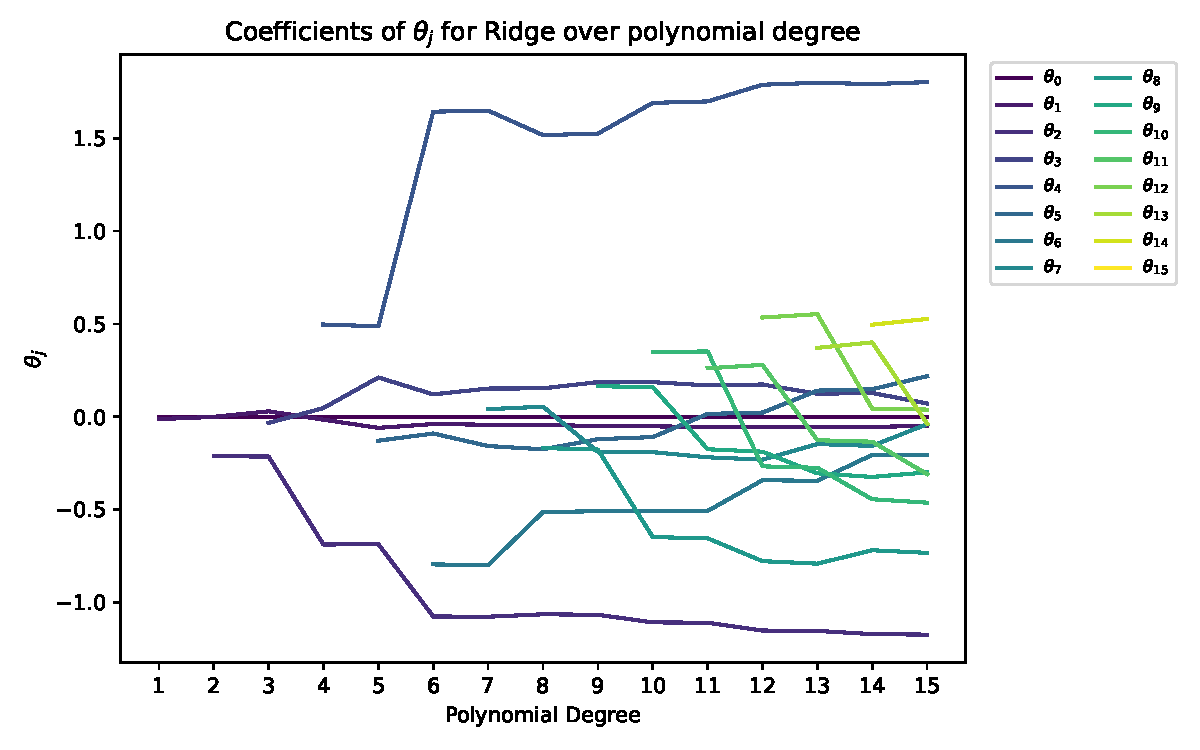
\includegraphics[width=\linewidth]{figs/Part_b_theta_vs_degree.pdf}
    \caption{Same data as in Figure \ref{fig:ols_theta_coeffs} but with penalty parameter 0.040. Visualization of how the penalty parameters suppresses the larger coefficients as all $\theta_j$} stay within [-1.0, 1.5]
    \label{fig:ridge_theta_coeff}
\end{figure}

\begin{figure}[h!]
    \centering
    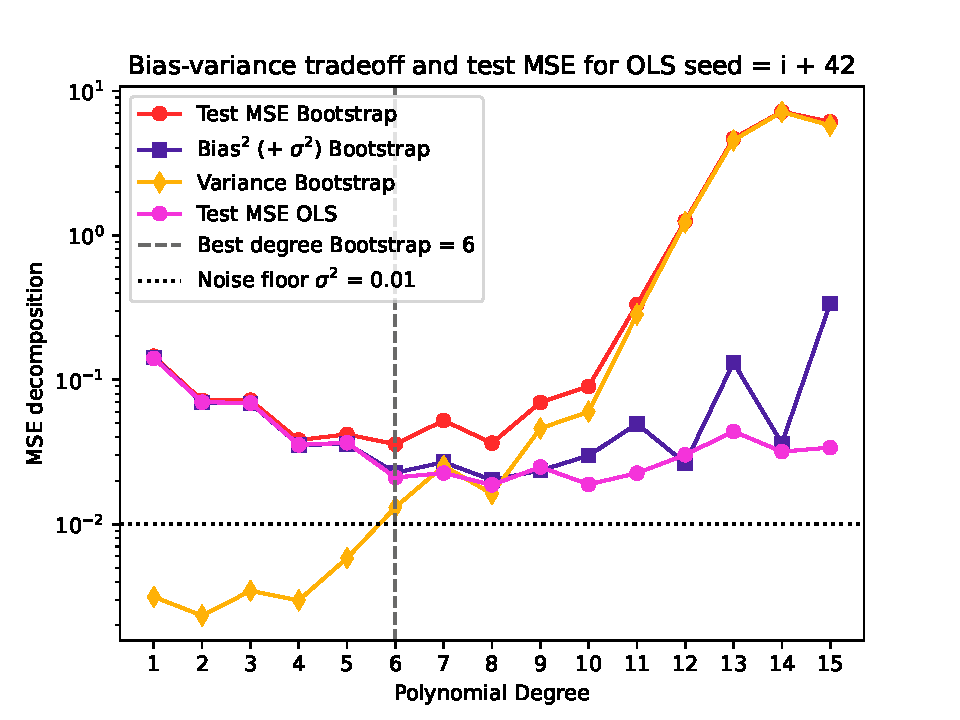
\includegraphics[width=\linewidth]{figs/Part_c_bootstrap_seed_42.pdf}
    \caption{Random state with seed = i + 42  in resampling for bootstraps changes the curves in the MSE decomposition and the optimal degree moves to degree 6}
    \label{fig:seed42}
\end{figure}



\begin{figure}[h!]
    \centering
    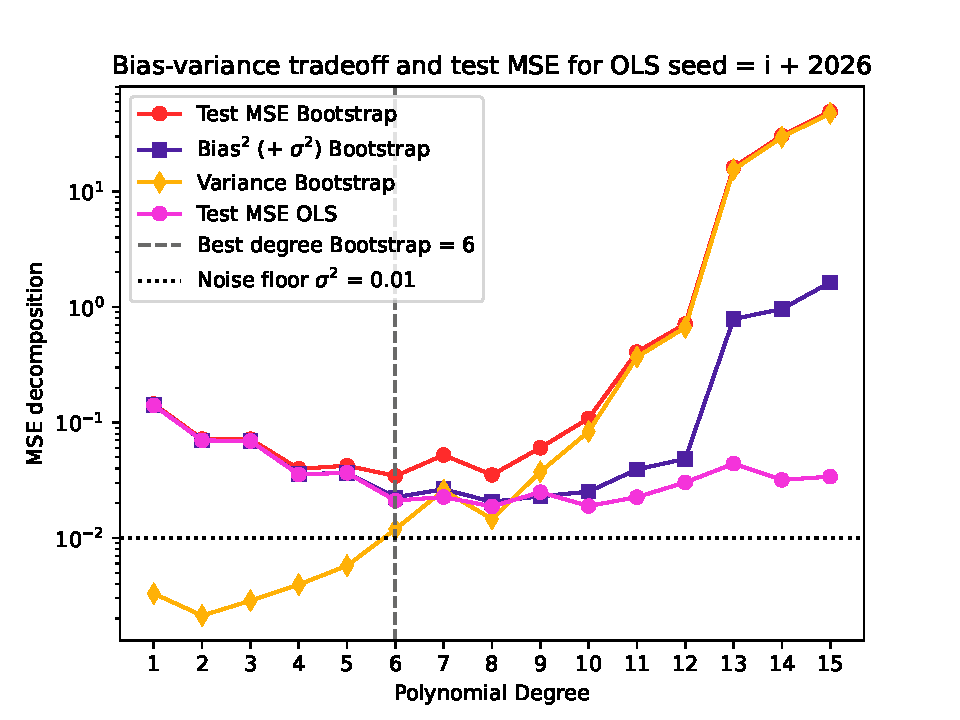
\includegraphics[width=\linewidth]{figs/Part_c_bootstrap_seed.pdf}
    \caption{Random state with seed = i + 2026  in resampling for bootstraps changes the curves in the MSE decomposition and the optimal degree moves to degree 6}
    \label{fig:seed2026}
\end{figure}



\begin{figure}[h!]
    \centering
    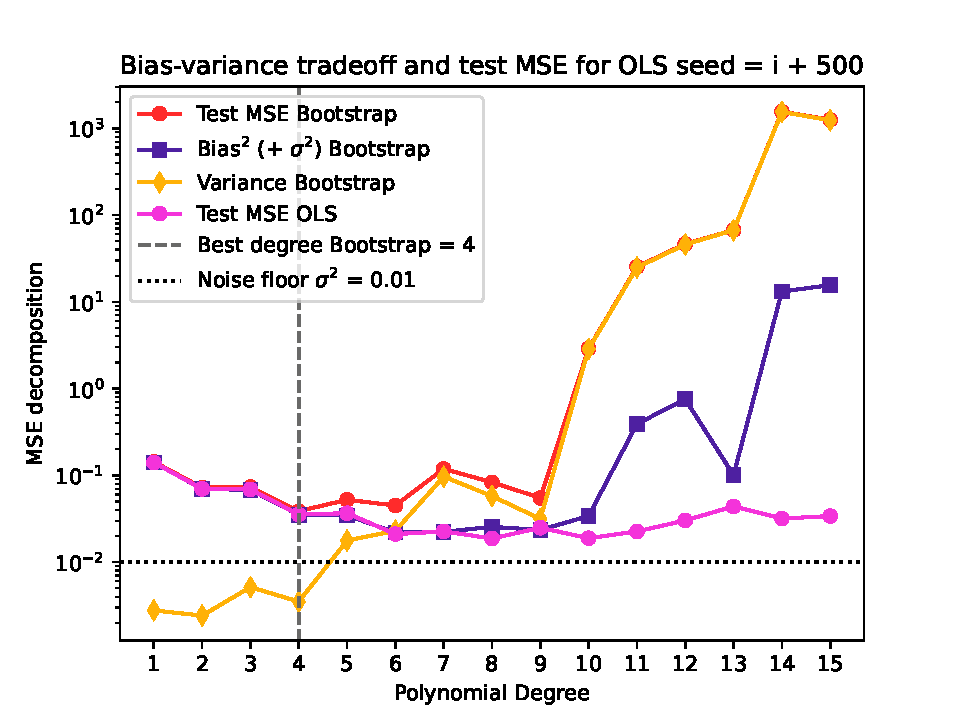
\includegraphics[width=\linewidth]{figs/Part_c_bootstrap_seed_500.pdf}
    \caption{Random state with seed = i + 500 in resampling for bootstraps changes the curves in the MSE decomposition and the optimal degree moves to degree 4}
    \label{fig:seed500}
\end{figure}




\clearpage
\onecolumngrid


\begin{figure}[htbp]
    \centering
    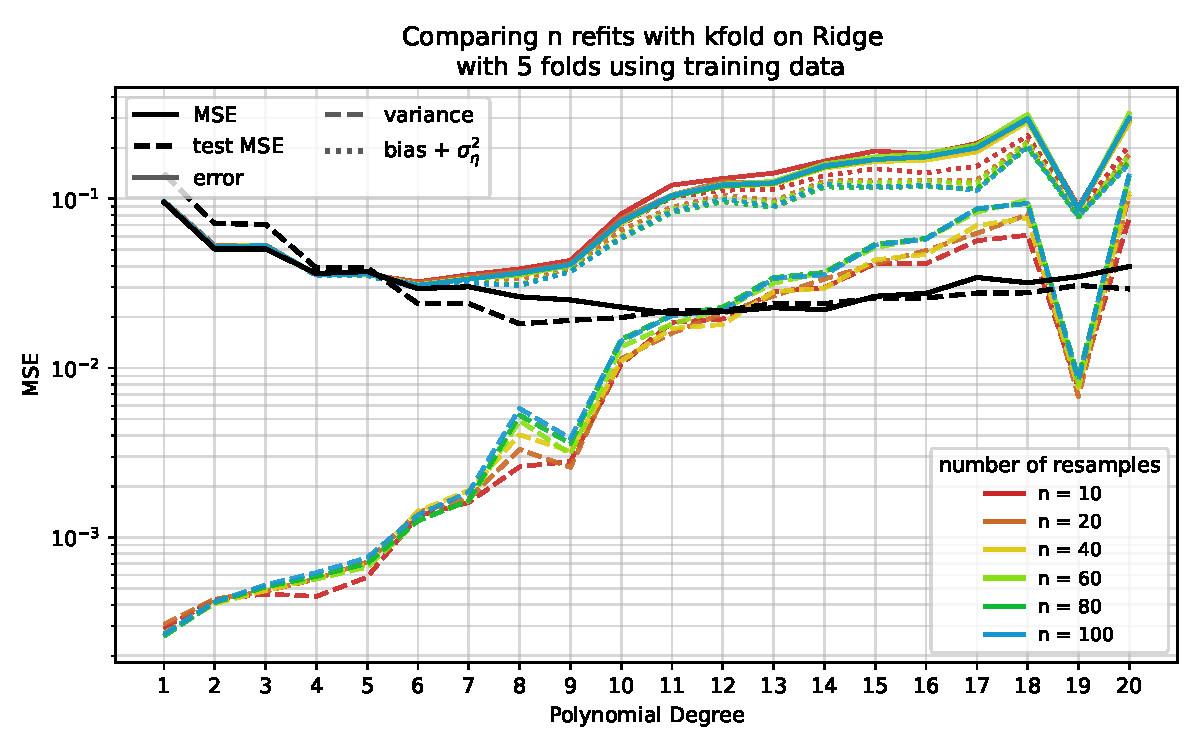
\includegraphics[width=0.48\textwidth]{figs/Part_i_hyperparameters_msedecomposition_kfold_resampling_clean_test_wholedatasetFalse.pdf}
    \hfill
    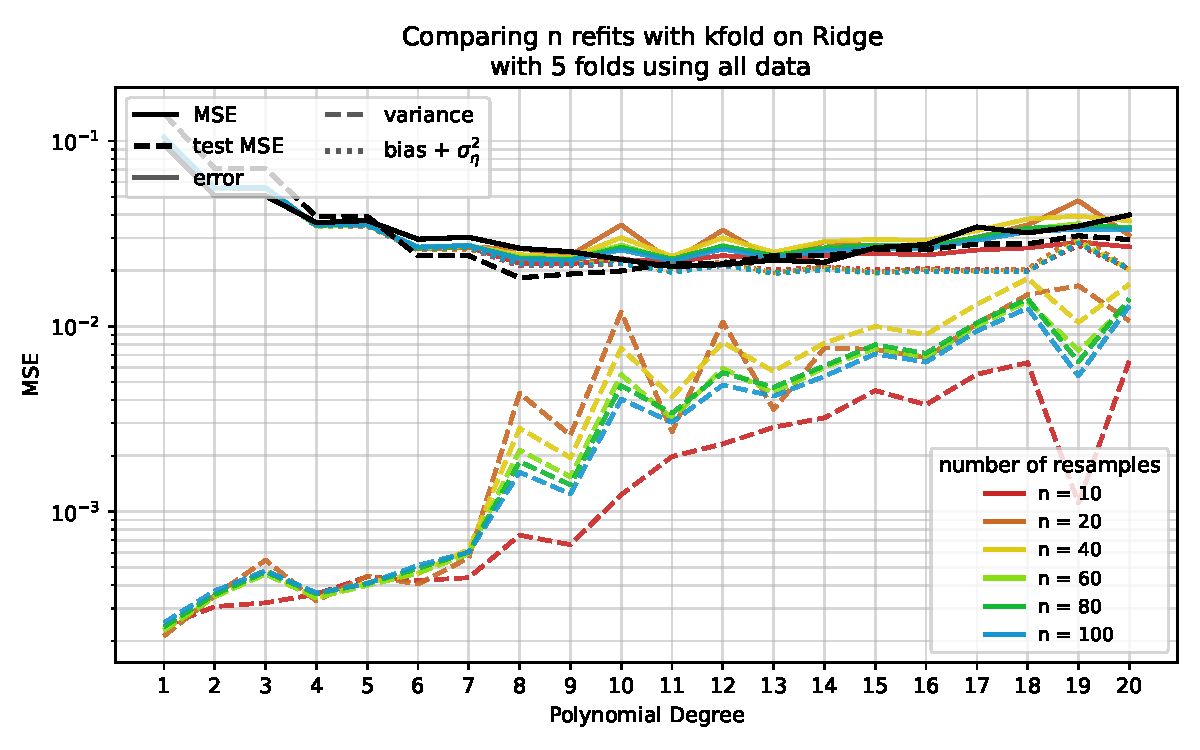
\includegraphics[width=0.48\textwidth]{figs/Part_i_hyperparameters_msedecomposition_kfold_resampling_clean_test_wholedatasetTrue.pdf}

    \vspace{1em}

    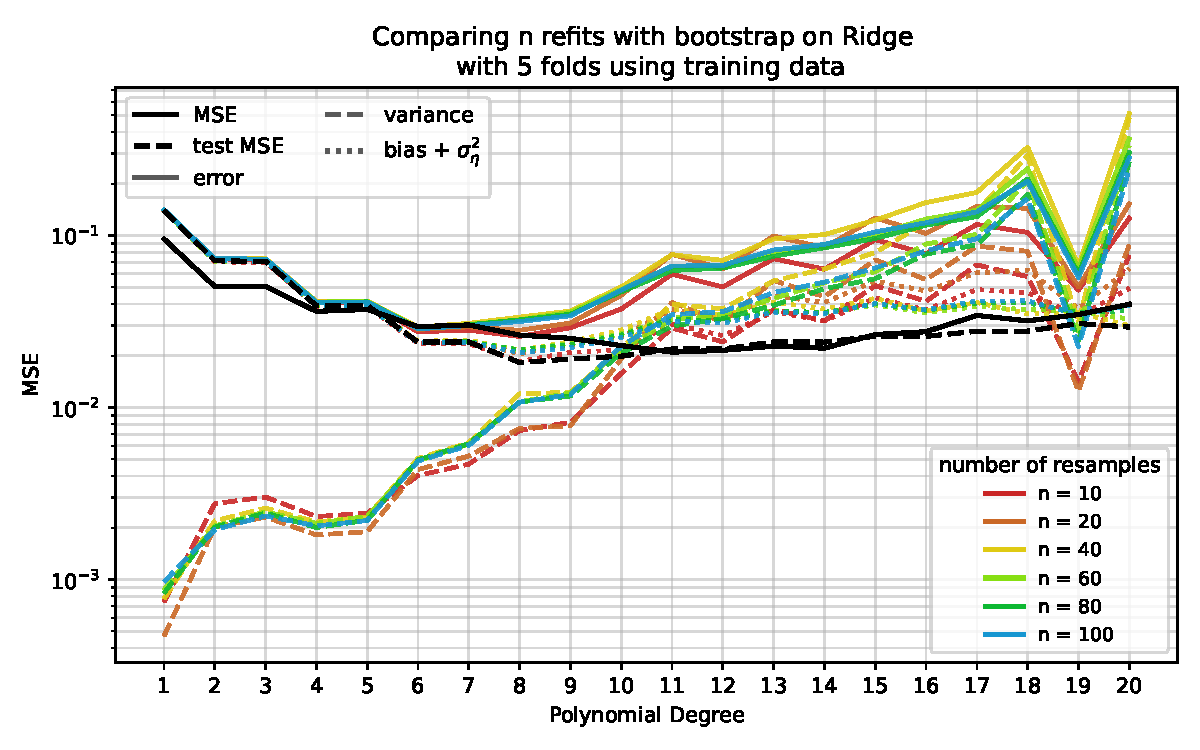
\includegraphics[width=0.48\textwidth]{figs/Part_i_hyperparameters_msedecomposition_bootstrap_resampling_clean_test_wholedatasetFalse.pdf}
    \hfill
    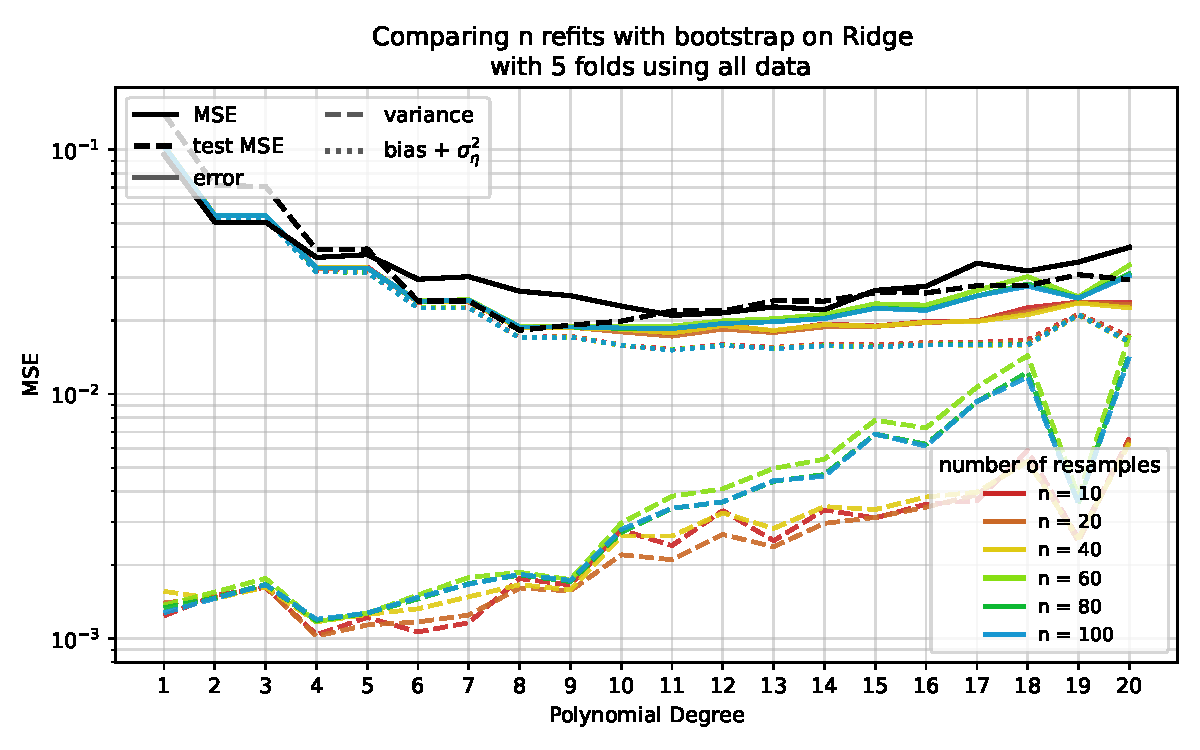
\includegraphics[width=0.48\textwidth]{figs/Part_i_hyperparameters_msedecomposition_bootstrap_resampling_clean_test_wholedatasetTrue.pdf}
\label{fig:apdx:MSE_decomposition}
\caption{Plots on the right show MSE decomposition using resampling on the training set, while those on the right show resampling on the whole set. Proper decomposition uses the same data as the training MSE gives, but this yields a terrible decomposition. An attempt was made using the whole training set. These match the training and testing MSEs better, but include more data than both have available. Clearly this MSE decomposition strategy was unfitting. The usage can be found in Tests\_and\_additional\_results/main\_test.ipynb with Code/resampling\_methods.py showing implementation of methods.}
\end{figure}

\end{document}

